\input{../_math_header.tex}
\usepackage[a4paper]{geometry}
\geometry{paperwidth=0.5\paperwidth,paperheight=100in,left=2em,right=2em,bottom=1em,top=2em}
\pagestyle{empty}
\setlength{\parindent}{0in}
\geometry{paperheight=250mm}


\usepackage{pgfpages}
\pagestyle{empty}
\pgfpagesuselayout{8 on 1}[a4paper,border shrink=0cm]
\makeatletter
\@tempcnta=1\relax
\loop\ifnum\@tempcnta<9\relax
\pgf@pset{\the\@tempcnta}{bordercode}{\pgfusepath{stroke}}
\advance\@tempcnta by 1\relax
\repeat
\makeatother


\usepackage[utf8]{inputenc}
\newenvironment{note}{\paragraph{NOTE:}}{\newpage}
\newenvironment{field}{\paragraph{}}{}
\newenvironment{plain}{\ttfamily}{\par}
\newcommand*{\xplain}[1]{\begin{itemize}\item \texttt{#1}\end{itemize}}
\newcommand*{\xfield}[1]{\begin{itemize}\item \texttt{#1}\end{itemize}}


    
\begin{document}

\section{Introduction}

\section{Classical probability}

\subsection{Classical probability}

%
\begin{note}
  \xplain{probability.tex 1}
  \begin{field}
    Classical probability
  \end{field}
  \begin{field}
    \begin{defi}[Classical probability]
      \emph{Classical probability} applies in a situation when there are a finite number of equally likely outcome.
    \end{defi}
  \end{field}
  \xplain{1.1 Classical probability}% Subsection
  \xplain{1 Classical probability}% Section
  \xplain{}% Subject
  \xplain{VOCABULARY}% Label
\end{note}

% To be manually edited
\begin{note}
  \xplain{probability.tex 2}
  \begin{field}
    \begin{eg}
      $A$ and $B$ play a game in which they keep throwing coins. If a head lands, then $A$ gets a point. Otherwise, $B$ gets a point. The first person to get 10 points wins a prize.
      Now suppose $A$ has got 8 points and $B$ has got 7, but the game has to end because an earthquake struck. How should they divide the prize? We answer this by finding the probability of $A$ winning. Someone must have won by the end of 19 rounds, i.e.\ after 4 more rounds. If $A$ wins at least 2 of them, then $A$ wins. Otherwise, $B$ wins.
      The number of ways this can happen is $\binom{4}{2} + \binom{4}{3} + \binom{4}{4} = 11$, while there are $16$ possible outcomes in total. So $A$ should get $11/16$ of the prize.
    \end{eg}
  \end{field}
  \begin{field}
    \begin{eg}
      $A$ and $B$ play a game in which they keep throwing coins. If a head lands, then $A$ gets a point. Otherwise, $B$ gets a point. The first person to get 10 points wins a prize.
      Now suppose $A$ has got 8 points and $B$ has got 7, but the game has to end because an earthquake struck. How should they divide the prize? We answer this by finding the probability of $A$ winning. Someone must have won by the end of 19 rounds, i.e.\ after 4 more rounds. If $A$ wins at least 2 of them, then $A$ wins. Otherwise, $B$ wins.
      The number of ways this can happen is $\binom{4}{2} + \binom{4}{3} + \binom{4}{4} = 11$, while there are $16$ possible outcomes in total. So $A$ should get $11/16$ of the prize.
    \end{eg}
  \end{field}
  \xplain{1.1 Classical probability}% Subsection
  \xplain{1 Classical probability}% Section
  \xplain{}% Subject
  \xplain{GENERAL KNOWLEDGE}% Label
\end{note}

%
\begin{note}
  \xplain{probability.tex 3}
  \begin{field}
    Sample space
  \end{field}
  \begin{field}
    \begin{defi}[Sample space]
      The set of all possible outcomes is the \emph{sample space}, $\Omega$. We can lists the outcomes as $\omega_1, \omega_2, \cdots \in \Omega$. Each $\omega \in \Omega$ is an \emph{outcome}.
    \end{defi}
  \end{field}
  \xplain{1.1 Classical probability}% Subsection
  \xplain{1 Classical probability}% Section
  \xplain{}% Subject
  \xplain{VOCABULARY}% Label
\end{note}

%
\begin{note}
  \xplain{probability.tex 4}
  \begin{field}
    Event
  \end{field}
  \begin{field}
    \begin{defi}[Event]
      A subset of $\Omega$ is called an \emph{event}.
    \end{defi}
  \end{field}
  \xplain{1.1 Classical probability}% Subsection
  \xplain{1 Classical probability}% Section
  \xplain{}% Subject
  \xplain{VOCABULARY}% Label
\end{note}

% To be manually edited
\begin{note}
  \xplain{probability.tex 5}
  \begin{field}
    \begin{eg}
      When rolling a dice, the sample space is $\{1, 2, 3, 4, 5, 6\}$, and each item is an outcome. ``Getting an odd number'' and ``getting 3'' are two possible events.
    \end{eg}
  \end{field}
  \begin{field}
    \begin{eg}
      When rolling a dice, the sample space is $\{1, 2, 3, 4, 5, 6\}$, and each item is an outcome. ``Getting an odd number'' and ``getting 3'' are two possible events.
    \end{eg}
  \end{field}
  \xplain{1.1 Classical probability}% Subsection
  \xplain{1 Classical probability}% Section
  \xplain{}% Subject
  \xplain{GENERAL KNOWLEDGE}% Label
\end{note}

%
\begin{note}
  \xplain{probability.tex 6}
  \begin{field}
    Set notations
  \end{field}
  \begin{field}
    \begin{defi}[Set notations]
      Given any two events $A, B\subseteq \Omega$,
      \begin{itemize}
        \item The \emph{complement} of $A$ is $A^C = A' = \bar A = \Omega\setminus A$.
        \item ``$A$ or $B$'' is the set $A\cup B$.
        \item ``$A$ and $B$'' is the set $A\cap B$.
        \item $A$ and $B$ are \emph{mutually exclusive} or \emph{disjoint} if $A\cap B = \emptyset$.
        \item If $A\subseteq B$, then $A$ occurring implies $B$ occurring.
      \end{itemize}
    \end{defi}
  \end{field}
  \xplain{1.1 Classical probability}% Subsection
  \xplain{1 Classical probability}% Section
  \xplain{}% Subject
  \xplain{VOCABULARY}% Label
\end{note}

%
\begin{note}
  \xplain{probability.tex 7}
  \begin{field}
    Probability
  \end{field}
  \begin{field}
    \begin{defi}[Probability]
      Suppose $\Omega = \{\omega_1,\omega_2, \cdots, \omega_N\}$. Let $A\subseteq \Omega$ be an event. Then the \emph{probability} of $A$ is
      \[
        \P(A) = \frac{\text{Number of outcomes in } A}{\text{Number of outcomes in }\Omega} = \frac{|A|}{N}.
      \]
    \end{defi}
  \end{field}
  \xplain{1.1 Classical probability}% Subsection
  \xplain{1 Classical probability}% Section
  \xplain{}% Subject
  \xplain{VOCABULARY}% Label
\end{note}

% To be manually edited
\begin{note}
  \xplain{probability.tex 8}
  \begin{field}
    \begin{eg}
      Suppose $r$ digits are drawn at random from a table of random digits from 0 to 9. What is the probability that
      \begin{enumerate}
        \item No digit exceeds $k$;
        \item The largest digit drawn is $k$?
      \end{enumerate}
      The sample space is $\Omega = \{(a_1, a_2, \cdots, a_r): 0 \leq a_i \leq 9\}$. Then $|\Omega| = 10^r$.
      Let $A_k = [\text{no digit exceeds }k] = \{(a_1, \cdots, a_r): 0 \leq a_i \leq k\}$. Then $|A_k| = (k + 1)^r$. So
      \[
        P(A_k) = \frac{(k + 1)^r}{10^r}.
      \]
      Now let $B_k = [\text{largest digit drawn is }k]$. We can find this by finding all outcomes in which no digits exceed $k$, and subtract it by the number of outcomes in which no digit exceeds $k - 1$. So $|B_k| = |A_k| - |A_{k - 1}|$ and
      \[
        P(B_k) = \frac{(k + 1)^r - k^r}{10^r}.
      \]
    \end{eg}
  \end{field}
  \begin{field}
    \begin{eg}
      Suppose $r$ digits are drawn at random from a table of random digits from 0 to 9. What is the probability that
      \begin{enumerate}
        \item No digit exceeds $k$;
        \item The largest digit drawn is $k$?
      \end{enumerate}
      The sample space is $\Omega = \{(a_1, a_2, \cdots, a_r): 0 \leq a_i \leq 9\}$. Then $|\Omega| = 10^r$.
      Let $A_k = [\text{no digit exceeds }k] = \{(a_1, \cdots, a_r): 0 \leq a_i \leq k\}$. Then $|A_k| = (k + 1)^r$. So
      \[
        P(A_k) = \frac{(k + 1)^r}{10^r}.
      \]
      Now let $B_k = [\text{largest digit drawn is }k]$. We can find this by finding all outcomes in which no digits exceed $k$, and subtract it by the number of outcomes in which no digit exceeds $k - 1$. So $|B_k| = |A_k| - |A_{k - 1}|$ and
      \[
        P(B_k) = \frac{(k + 1)^r - k^r}{10^r}.
      \]
    \end{eg}
  \end{field}
  \xplain{1.1 Classical probability}% Subsection
  \xplain{1 Classical probability}% Section
  \xplain{}% Subject
  \xplain{GENERAL KNOWLEDGE}% Label
\end{note}

\subsection{Counting}

% To be manually edited
\begin{note}
  \xplain{probability.tex 9}
  \begin{field}
    \begin{eg}
      A menu has 6 starters, 7 mains and 6 desserts. How many possible meals combinations are there? Clearly $6 \times 7 \times 6 = 252$.
    \end{eg}
  \end{field}
  \begin{field}
    \begin{eg}
      A menu has 6 starters, 7 mains and 6 desserts. How many possible meals combinations are there? Clearly $6 \times 7 \times 6 = 252$.
    \end{eg}
  \end{field}
  \xplain{1.2 Counting}% Subsection
  \xplain{1 Classical probability}% Section
  \xplain{}% Subject
  \xplain{GENERAL KNOWLEDGE}% Label
\end{note}

%
\begin{note}
  \xplain{probability.tex 10}
  \begin{field}
    Fundamental rule of counting
  \end{field}
  \begin{field}
    \begin{thm}[Fundamental rule of counting]
      Suppose we have to make $r$ multiple choices in sequence. There are $m_1$ possibilities for the first choice, $m_2$ possibilities for the second etc. Then the total number of choices is $m_1\times m_2\times \cdots m_r$.
    \end{thm}
  \end{field}
  \xplain{1.2 Counting}% Subsection
  \xplain{1 Classical probability}% Section
  \xplain{}% Subject
  \xplain{GENERAL KNOWLEDGE}% Label
\end{note}

% To be manually edited
\begin{note}
  \xplain{probability.tex 11}
  \begin{field}
    \begin{eg}
      How many ways can $1, 2, \cdots, n$ be ordered? The first choice has $n$ possibilities, the second has $n - 1$ possibilities etc. So there are $n\times (n - 1)\times\cdots \times 1 = n!$.
    \end{eg}
  \end{field}
  \begin{field}
    \begin{eg}
      How many ways can $1, 2, \cdots, n$ be ordered? The first choice has $n$ possibilities, the second has $n - 1$ possibilities etc. So there are $n\times (n - 1)\times\cdots \times 1 = n!$.
    \end{eg}
  \end{field}
  \xplain{1.2 Counting}% Subsection
  \xplain{1 Classical probability}% Section
  \xplain{}% Subject
  \xplain{GENERAL KNOWLEDGE}% Label
\end{note}

%
\begin{note}
  \xplain{probability.tex 12}
  \begin{field}
    Sampling with replacement
  \end{field}
  \begin{field}
    \begin{defi}[Sampling with replacement]
      When we \emph{sample with replacement}, after choosing at item, it is put back and can be chosen again. Then \emph{any} sampling function $f$ satisfies sampling with replacement.
    \end{defi}
  \end{field}
  \xplain{1.2 Counting}% Subsection
  \xplain{1 Classical probability}% Section
  \xplain{}% Subject
  \xplain{VOCABULARY}% Label
\end{note}

%
\begin{note}
  \xplain{probability.tex 13}
  \begin{field}
    Sampling without replacement
  \end{field}
  \begin{field}
    \begin{defi}[Sampling without replacement]
      When we \emph{sample without replacement}, after choosing an item, we kill it with fire and cannot choose it again. Then $f$ must be an injective function, and clearly we must have $x \geq n$.
    \end{defi}
  \end{field}
  \xplain{1.2 Counting}% Subsection
  \xplain{1 Classical probability}% Section
  \xplain{}% Subject
  \xplain{VOCABULARY}% Label
\end{note}

% To be manually edited
\begin{note}
  \xplain{probability.tex 14}
  \begin{field}
    \begin{eg}
      Suppose $N = \{a, b, c\}$ and $X = \{p, q, r, s\}$. How many injective functions are there $N\to X$?
      When we choose $f(a)$, we have 4 options. When we choose $f(b)$, we have 3 left. When we choose $f(c)$, we have 2 choices left. So there are $24$ possible choices.
    \end{eg}
  \end{field}
  \begin{field}
    \begin{eg}
      Suppose $N = \{a, b, c\}$ and $X = \{p, q, r, s\}$. How many injective functions are there $N\to X$?
      When we choose $f(a)$, we have 4 options. When we choose $f(b)$, we have 3 left. When we choose $f(c)$, we have 2 choices left. So there are $24$ possible choices.
    \end{eg}
  \end{field}
  \xplain{1.2 Counting}% Subsection
  \xplain{1 Classical probability}% Section
  \xplain{}% Subject
  \xplain{GENERAL KNOWLEDGE}% Label
\end{note}

% To be manually edited
\begin{note}
  \xplain{probability.tex 15}
  \begin{field}
    \begin{eg}
      I have $n$ keys in my pocket. We select one at random once and try to unlock. What is the possibility that I succeed at the $r$th trial?
      Suppose we do it with replacement. We have to fail the first $r - 1$ trials and succeed in the $r$th. So the probability is
      \[
        \frac{(n - 1)(n - 1) \cdots (n - 1)(1)}{n^r} = \frac{(n - 1)^{r - 1}}{n^r}.
      \]
      Now suppose we are smarter and try without replacement. Then the probability is
      \[
        \frac{(n - 1)(n - 2)\cdots (n - r + 1)(1)}{n(n - 1) \cdots (n - r + 1)} = \frac{1}{n}.
      \]
    \end{eg}
  \end{field}
  \begin{field}
    \begin{eg}
      I have $n$ keys in my pocket. We select one at random once and try to unlock. What is the possibility that I succeed at the $r$th trial?
      Suppose we do it with replacement. We have to fail the first $r - 1$ trials and succeed in the $r$th. So the probability is
      \[
        \frac{(n - 1)(n - 1) \cdots (n - 1)(1)}{n^r} = \frac{(n - 1)^{r - 1}}{n^r}.
      \]
      Now suppose we are smarter and try without replacement. Then the probability is
      \[
        \frac{(n - 1)(n - 2)\cdots (n - r + 1)(1)}{n(n - 1) \cdots (n - r + 1)} = \frac{1}{n}.
      \]
    \end{eg}
  \end{field}
  \xplain{1.2 Counting}% Subsection
  \xplain{1 Classical probability}% Section
  \xplain{}% Subject
  \xplain{GENERAL KNOWLEDGE}% Label
\end{note}

%
\begin{note}
  \xplain{probability.tex 16}
  \begin{field}
    Birthday problem
  \end{field}
  \begin{field}
    \begin{eg}[Birthday problem]
      How many people are needed in a room for there to be a probability that two people have the same birthday to be at least a half?
      Suppose $f(r)$ is the probability that, in a room of $r$ people, there is a birthday match.
      We solve this by finding the probability of no match, $1 - f(r)$. The total number of possibilities of birthday combinations is $365^r$. For nobody to have the same birthday, the first person can have any birthday. The second has 364 else to choose, etc. So
      \[
        \P(\text{no match}) = \frac{365\cdot 364\cdot 363 \cdots (366 - r)}{365\cdot 365\cdot 365 \cdots 365}.
      \]
      If we calculate this with a computer, we find that $f(22) = 0.475695$ and $f(23) = 0.507297$.
      While this might sound odd since 23 is small, this is because we are thinking about the wrong thing. The probability of match is related more to the number of \emph{pairs} of people, not the number of people. With 23 people, we have $23\times 22/2 = 253$ pairs, which is quite large compared to 365.
    \end{eg}
  \end{field}
  \xplain{1.2 Counting}% Subsection
  \xplain{1 Classical probability}% Section
  \xplain{}% Subject
  \xplain{GENERAL KNOWLEDGE}% Label
\end{note}

%
\begin{note}
  \xplain{probability.tex 17}
  \begin{field}
    Multinomial coefficient
  \end{field}
  \begin{field}
    \begin{defi}[Multinomial coefficient]
      A \emph{multinomial coefficient} is
      \[
        \binom{n}{n_1, n_2, \cdots, n_k} = \binom{n}{n_1}\binom{n - n_1}{n_2}\cdots \binom{n - n_1\cdots - n_{k - 1}}{n_k} = \frac{n!}{n_1!n_2!\cdots n_k!}.
      \]
      It is the number of ways to distribute $n$ items into $k$ positions, in which the $i$th position has $n_i$ items.
    \end{defi}
  \end{field}
  \xplain{1.2 Counting}% Subsection
  \xplain{1 Classical probability}% Section
  \xplain{}% Subject
  \xplain{VOCABULARY}% Label
\end{note}

% To be manually edited
\begin{note}
  \xplain{probability.tex 18}
  \begin{field}
    \begin{eg}
      We know that
      \[
        (x + y)^n = x^n + \binom{n}{1}x^{n - 1}y + \cdots + y^n.
      \]
      If we have a trinomial, then
      \[
        (x + y + z)^n = \sum_{n_1, n_2, n_3} \binom{n}{n_1, n_2, n_3} x^{n_1}y^{n_2}z^{n_3}.
      \]
    \end{eg}
  \end{field}
  \begin{field}
    \begin{eg}
      We know that
      \[
        (x + y)^n = x^n + \binom{n}{1}x^{n - 1}y + \cdots + y^n.
      \]
      If we have a trinomial, then
      \[
        (x + y + z)^n = \sum_{n_1, n_2, n_3} \binom{n}{n_1, n_2, n_3} x^{n_1}y^{n_2}z^{n_3}.
      \]
    \end{eg}
  \end{field}
  \xplain{1.2 Counting}% Subsection
  \xplain{1 Classical probability}% Section
  \xplain{}% Subject
  \xplain{GENERAL KNOWLEDGE}% Label
\end{note}

% To be manually edited
\begin{note}
  \xplain{probability.tex 19}
  \begin{field}
    \begin{eg}
      How many ways can we deal 52 cards to 4 player, each with a hand of 13? The total number of ways is
      \[
        \binom{52}{13, 13, 13, 13} = \frac{52!}{(13!)^4} = 53644737765488792839237440000 = 5.36\times 10^{28}.
      \]
    \end{eg}
  \end{field}
  \begin{field}
    \begin{eg}
      How many ways can we deal 52 cards to 4 player, each with a hand of 13? The total number of ways is
      \[
        \binom{52}{13, 13, 13, 13} = \frac{52!}{(13!)^4} = 53644737765488792839237440000 = 5.36\times 10^{28}.
      \]
    \end{eg}
  \end{field}
  \xplain{1.2 Counting}% Subsection
  \xplain{1 Classical probability}% Section
  \xplain{}% Subject
  \xplain{GENERAL KNOWLEDGE}% Label
\end{note}

\subsection{Stirling's formula}

% To be manually edited
\begin{note}
  \xplain{probability.tex 20}
  \begin{field}
    \begin{prop}
      $\log n!\sim n\log n$
    \end{prop}
  \end{field}
  \begin{field}
    \begin{prop}
      $\log n!\sim n\log n$
    \end{prop}
  \end{field}
  \xplain{1.3 Stirling's formula}% Subsection
  \xplain{1 Classical probability}% Section
  \xplain{}% Subject
  \xplain{GENERAL KNOWLEDGE}% Label
\end{note}

%
\begin{note}
  \xplain{probability.tex 21}
  \begin{field}
    \begin{prop}
      $\log n!\sim n\log n$
    \end{prop}
  \end{field}
  \begin{field}
    \begin{proof}
      Note that
      \[
        \log n! = \sum_{k=1}^n \log k.
      \]
      Now we claim that
      \[
        \int_1^n \log x\;\d x \leq \sum_1^n \log k\leq \int_1^{n + 1}\log x\;\d x.
      \]
      This is true by considering the diagram:
      \begin{center}
        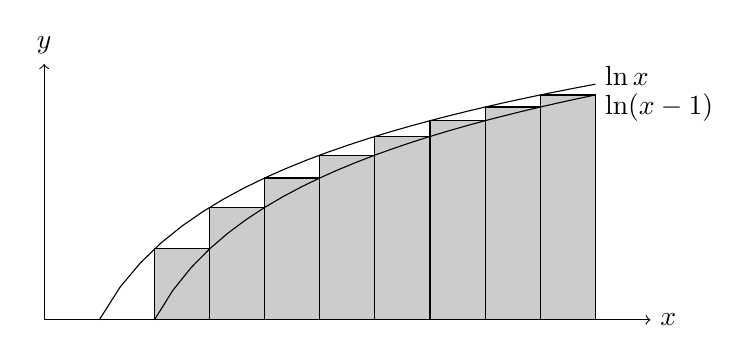
\begin{tikzpicture}[xscale=0.7, yscale=1.3]
         \draw [->] (0, 0) -- (11, 0) node [right] {$x$};
         \draw [->] (0, 0) -- (0, 2.5) node [above] {$y$};
         \draw [domain=2:10] plot (\x, {ln (\x - 1)}) node [anchor = south west] {$\ln x$};
         \draw [domain=1:10] plot (\x, {ln \x }) node [anchor = north west] {$\ln (x - 1)$};
         \draw [fill = black, fill opacity=0.2] (2, 0)-- (2, 0.693147180559945) -- (3, 0.693147180559945) -- (3, 0);
         \draw [fill = black, fill opacity=0.2] (3, 0)-- (3, 1.09861228866811) -- (4, 1.09861228866811) -- (4, 0);
         \draw [fill = black, fill opacity=0.2] (4, 0)-- (4, 1.38629436111989) -- (5, 1.38629436111989) -- (5, 0);
         \draw [fill = black, fill opacity=0.2] (5, 0)-- (5, 1.6094379124341) -- (6, 1.6094379124341) -- (6, 0);
         \draw [fill = black, fill opacity=0.2] (6, 0)-- (6, 1.79175946922806) -- (7, 1.79175946922806) -- (7, 0);
         \draw [fill = black, fill opacity=0.2] (7, 0)-- (7, 1.94591014905531) -- (8, 1.94591014905531) -- (8, 0);
         \draw [fill = black, fill opacity=0.2] (8, 0)-- (8, 2.07944154167984) -- (9, 2.07944154167984) -- (9, 0);
         \draw [fill = black, fill opacity=0.2] (9, 0)-- (9, 2.19722457733622) -- (10, 2.19722457733622) -- (10, 0);
        \end{tikzpicture}
      \end{center}
      We actually evaluate the integral to obtain
      \[
        n\log n - n + 1 \leq \log n! \leq (n+ 1)\log (n + 1) - n;
      \]
      Divide both sides by $n\log n$ and let $n\to \infty$. Both sides tend to $1$. So
      \[
        \frac{\log n!}{n\log n} \to 1.\qedhere
      \]
    \end{proof}
  \end{field}
  \xplain{1.3 Stirling's formula}% Subsection
  \xplain{1 Classical probability}% Section
  \xplain{}% Subject
  \xplain{PROOF EXERCISE}% Label
\end{note}

%
\begin{note}
  \xplain{probability.tex 22}
  \begin{field}
    Stirling's formula
  \end{field}
  \begin{field}
    \begin{thm}[Stirling's formula]
      As $n\to \infty$,
      \[
        \log\left(\frac{n! e^n}{n^{n + \frac{1}{2}}}\right) = \log \sqrt{2\pi} + O\left(\frac{1}{n}\right)
      \]
    \end{thm}
  \end{field}
  \xplain{1.3 Stirling's formula}% Subsection
  \xplain{1 Classical probability}% Section
  \xplain{}% Subject
  \xplain{GENERAL KNOWLEDGE}% Label
\end{note}

% To be manually edited
\begin{note}
  \xplain{probability.tex 23}
  \begin{field}
    \begin{cor}
      \[
        n!\sim \sqrt{2\pi}n^{n + \frac{1}{2}} e^{-n}
      \]
    \end{cor}
  \end{field}
  \begin{field}
    \begin{cor}
      \[
        n!\sim \sqrt{2\pi}n^{n + \frac{1}{2}} e^{-n}
      \]
    \end{cor}
  \end{field}
  \xplain{1.3 Stirling's formula}% Subsection
  \xplain{1 Classical probability}% Section
  \xplain{}% Subject
  \xplain{GENERAL KNOWLEDGE}% Label
\end{note}

%
\begin{note}
  \xplain{probability.tex 24}
  \begin{field}
    \begin{cor}
      \[
        n!\sim \sqrt{2\pi}n^{n + \frac{1}{2}} e^{-n}
      \]
    \end{cor}
  \end{field}
  \begin{field}
    \begin{proof}(non-examinable)
      Define
      \[
        d_n = \log \left(\frac{n!e^n}{n^{n + 1/2}}\right) = \log n! - (n + 1/2)\log n + n
      \]
      Then
      \[
        d_n - d_{n + 1} = (n + 1/2)\log\left(\frac{n + 1}{n}\right) - 1.
      \]
      Write $t = 1/(2n + 1)$. Then
      \[
        d_n - d_{n + 1} = \frac{1}{2t}\log\left(\frac{1 + t}{1 - t}\right) - 1.
      \]
      We can simplifying by noting that
      \begin{align*}
        \log (1 + t) - t &= -\frac{1}{2}t^2 + \frac{1}{3}t^3 - \frac{1}{4}t^4 + \cdots\\
        \log (1 - t) + t &= -\frac{1}{2}t^2 - \frac{1}{3}t^3 - \frac{1}{4}t^4 - \cdots
      \end{align*}
      Then if we subtract the equations and divide by $2t$, we obtain
      \begin{align*}
        d_n - d_{n + 1} &= \frac{1}{3}t^2 + \frac{1}{5}t^4 + \frac{1}{7}t^6 + \cdots\\
        &< \frac{1}{3}t^2 + \frac{1}{3}t^4 + \frac{1}{3}t^6 + \cdots\\
        &= \frac{1}{3}\frac{t^2}{1 - t^2}\\
        &= \frac{1}{3}\frac{1}{(2n + 1)^2 - 1}\\
        &= \frac{1}{12}\left(\frac{1}{n} - \frac{1}{n + 1}\right)
      \end{align*}
      By summing these bounds, we know that
      \[
        d_1 - d_n < \frac{1}{12}\left(1 - \frac{1}{n}\right)
      \]
      Then we know that $d_n$ is bounded below by $d_1 +$ something, and is decreasing since $d_n - d_{n + 1}$ is positive. So it converges to a limit $A$. We know $A$ is a lower bound for $d_n$ since $(d_n)$ is decreasing.
      Suppose $m > n$. Then $d_n - d_m < \left(\frac{1}{n} - \frac{1}{m}\right)\frac{1}{12}$. So taking the limit as $m\to \infty$, we obtain an upper bound for $d_n$: $d_n < A + 1/(12n)$. Hence we know that
      \[
        A < d_n < A + \frac{1}{12n}.
      \]
      However, all these results are useless if we don't know what $A$ is. To find $A$, we have a small detour to prove a formula:
      Take $I_n = \int_0^{\pi/2} \sin^n\theta\;\d \theta$. This is decreasing for increasing $n$ as $\sin^n\theta$ gets smaller. We also know that
      \begin{align*}
        I_n &= \int_0^{\pi/2}\sin^n \theta\;\d \theta\\
        &= \left[-\cos\theta\sin^{n - 1}\theta \right]_0^{\pi/2} + \int_0^{\pi/2} (n - 1)\cos^2\theta \sin^{n - 2}\theta \;\d\theta\\
        &= 0 + \int_0^{\pi/2}(n - 1)(1 - \sin^2 \theta)\sin^{n - 2}\theta \;\d \theta\\
        &= (n - 1)(I_{n - 2} - I_n)
      \end{align*}
      So
      \[
        I_n = \frac{n - 1}{n}I_{n - 2}.
      \]
      We can directly evaluate the integral to obtain $I_0 = \pi/2$, $I_1 = 1$. Then
      \begin{align*}
        I_{2n} &= \frac{1}{2}\cdot\frac{3}{4}\cdots \frac{2n - 1}{2n} \pi/2 = \frac{(2n)!}{(2^nn!)^2}\frac{\pi}{2}\\
        I_{2n + 1} &= \frac{2}{3}\cdot\frac{4}{5}\cdots\frac{2n}{2n + 1} = \frac{(2^nn!)^2}{(2n + 1)!}
      \end{align*}
      So using the fact that $I_n$ is decreasing, we know that
      \[
        1 \leq \frac{I_{2n}}{I_{2n + 1}} \leq \frac{I_{2n - 1}}{I_{2n + 1}} = 1 + \frac{1}{2n} \to 1.
      \]
      Using the approximation $n!\sim n^{n + 1/2}e^{-n + A}$, where $A$ is the limit we want to find, we can approximate
      \[
        \frac{I_{2n}}{I_{2n + 1}} = \pi(2n + 1)\left[\frac{( (2n)!)^2}{2^{4n + 1}(n!)^4}\right] \sim \pi(2n + 1)\frac{1}{ne^{2A}}\to \frac{2\pi}{e^{2A}}.
      \]
      Since the last expression is equal to 1, we know that $A = \log\sqrt{2\pi}$. Hooray for magic!
    \end{proof}
  \end{field}
  \xplain{1.3 Stirling's formula}% Subsection
  \xplain{1 Classical probability}% Section
  \xplain{}% Subject
  \xplain{PROOF EXERCISE}% Label
\end{note}

%
\begin{note}
  \xplain{probability.tex 25}
  \begin{field}
    non-examinable
  \end{field}
  \begin{field}
    \begin{prop}[non-examinable]
      We use the $1/12n$ term from the proof above to get a better approximation:
      \[
        \sqrt{2\pi}n^{n + 1/2}e^{-n + \frac{1}{12n + 1}} \leq n! \leq \sqrt{2\pi} n^{n + 1/2} e^{-n + \frac{1}{12n}}.
      \]
    \end{prop}
  \end{field}
  \xplain{1.3 Stirling's formula}% Subsection
  \xplain{1 Classical probability}% Section
  \xplain{}% Subject
  \xplain{GENERAL KNOWLEDGE}% Label
\end{note}

% To be manually edited
\begin{note}
  \xplain{probability.tex 26}
  \begin{field}
    \begin{eg}
      Suppose we toss a coin $2n$ times. What is the probability of equal number of heads and tails? The probability is
      \[
        \frac{\binom{2n}{n}}{2^{2n}} = \frac{(2n)!}{(n!)^2 2^{2n}} \sim \frac{1}{\sqrt{n\pi}}
      \]
    \end{eg}
  \end{field}
  \begin{field}
    \begin{eg}
      Suppose we toss a coin $2n$ times. What is the probability of equal number of heads and tails? The probability is
      \[
        \frac{\binom{2n}{n}}{2^{2n}} = \frac{(2n)!}{(n!)^2 2^{2n}} \sim \frac{1}{\sqrt{n\pi}}
      \]
    \end{eg}
  \end{field}
  \xplain{1.3 Stirling's formula}% Subsection
  \xplain{1 Classical probability}% Section
  \xplain{}% Subject
  \xplain{GENERAL KNOWLEDGE}% Label
\end{note}

% To be manually edited
\begin{note}
  \xplain{probability.tex 27}
  \begin{field}
    \begin{eg}
      Suppose we draw 26 cards from 52. What is the probability of getting 13 reds and 13 blacks? The probability is
      \[
        \frac{\binom{26}{13}\binom{26}{13}}{\binom{52}{26}} = 0.2181.
      \]
    \end{eg}
  \end{field}
  \begin{field}
    \begin{eg}
      Suppose we draw 26 cards from 52. What is the probability of getting 13 reds and 13 blacks? The probability is
      \[
        \frac{\binom{26}{13}\binom{26}{13}}{\binom{52}{26}} = 0.2181.
      \]
    \end{eg}
  \end{field}
  \xplain{1.3 Stirling's formula}% Subsection
  \xplain{1 Classical probability}% Section
  \xplain{}% Subject
  \xplain{GENERAL KNOWLEDGE}% Label
\end{note}

\section{Axioms of probability}

\subsection{Axioms and definitions}

% To be manually edited
\begin{note}
  \xplain{probability.tex 28}
  \begin{field}
    \begin{defi}[Probability space]
      A \emph{probability space} is a triple $(\Omega, \mathcal{F}, \P)$. $\Omega$ is a set called the \emph{sample space}, $\mathcal{F}$ is a collection of subsets of $\Omega$, and $\P: \mathcal{F}\to [0, 1]$ is the \emph{probability measure}.
      $\mathcal{F}$ has to satisfy the following axioms:
      \begin{enumerate}
        \item $\emptyset, \Omega\in \mathcal{F}$.
        \item $A\in \mathcal{F} \Rightarrow A^C\in \mathcal{F}$.
        \item $A_1, A_2, \cdots \in \mathcal{F} \Rightarrow \bigcup_{i = 1}^\infty A_i \in \mathcal{F}$.
      \end{enumerate}
      And $\P$ has to satisfy the following \emph{Kolmogorov axioms}:
      \begin{enumerate}
        \item $0 \leq \P(A) \leq 1 $ for all $A\in \mathcal{F}$
        \item $\P(\Omega) = 1$
        \item For any countable collection of events $A_1, A_2, \cdots$ which are disjoint, i.e.\ $A_i\cap A_j = \emptyset$ for all $i, j$, we have
          \[
            \P\left(\bigcup_i A_i\right) = \sum_i \P(A_i).
          \]
      \end{enumerate}
      Items in $\Omega$ are known as the \emph{outcomes}, items in $\mathcal{F}$ are known as the \emph{events}, and $\P(A)$ is the \emph{probability} of the event $A$.
    \end{defi}
  \end{field}
  \begin{field}
    \begin{defi}[Probability space]
      A \emph{probability space} is a triple $(\Omega, \mathcal{F}, \P)$. $\Omega$ is a set called the \emph{sample space}, $\mathcal{F}$ is a collection of subsets of $\Omega$, and $\P: \mathcal{F}\to [0, 1]$ is the \emph{probability measure}.
      $\mathcal{F}$ has to satisfy the following axioms:
      \begin{enumerate}
        \item $\emptyset, \Omega\in \mathcal{F}$.
        \item $A\in \mathcal{F} \Rightarrow A^C\in \mathcal{F}$.
        \item $A_1, A_2, \cdots \in \mathcal{F} \Rightarrow \bigcup_{i = 1}^\infty A_i \in \mathcal{F}$.
      \end{enumerate}
      And $\P$ has to satisfy the following \emph{Kolmogorov axioms}:
      \begin{enumerate}
        \item $0 \leq \P(A) \leq 1 $ for all $A\in \mathcal{F}$
        \item $\P(\Omega) = 1$
        \item For any countable collection of events $A_1, A_2, \cdots$ which are disjoint, i.e.\ $A_i\cap A_j = \emptyset$ for all $i, j$, we have
          \[
            \P\left(\bigcup_i A_i\right) = \sum_i \P(A_i).
          \]
      \end{enumerate}
      Items in $\Omega$ are known as the \emph{outcomes}, items in $\mathcal{F}$ are known as the \emph{events}, and $\P(A)$ is the \emph{probability} of the event $A$.
    \end{defi}
  \end{field}
  \xplain{2.1 Axioms and definitions}% Subsection
  \xplain{2 Axioms of probability}% Section
  \xplain{}% Subject
  \xplain{VOCABULARY}% Label
\end{note}

%
\begin{note}
  \xplain{probability.tex 29}
  \begin{field}
    Probability distribution
  \end{field}
  \begin{field}
    \begin{defi}[Probability distribution]
      Let $\Omega = \{\omega_1, \omega_2, \cdots\}$. Choose numbers $p_1, p_2, \cdots $ such that $\sum_{i = 1}^\infty p_i= 1$. Let $p(\omega_i) = p_i$. Then define
      \[
        \P(A) = \sum_{\omega_i\in A} p(\omega_i).
      \]
      This $\P(A)$ satisfies the above axioms, and $p_1, p_2, \cdots$ is the \emph{probability distribution}
    \end{defi}
  \end{field}
  \xplain{2.1 Axioms and definitions}% Subsection
  \xplain{2 Axioms of probability}% Section
  \xplain{}% Subject
  \xplain{VOCABULARY}% Label
\end{note}

% To be manually edited
\begin{note}
  \xplain{probability.tex 30}
  \begin{field}
    \begin{thm}\leavevmode
      \begin{enumerate}
        \item $\P(\emptyset) = 0$
        \item $\P(A^C) = 1 - \P(A)$
        \item $A\subseteq B \Rightarrow \P(A) \leq \P(B)$
        \item $\P (A\cup B) = \P(A) + \P(B) - \P(A\cap B)$.
      \end{enumerate}
    \end{thm}
  \end{field}
  \begin{field}
    \begin{thm}\leavevmode
      \begin{enumerate}
        \item $\P(\emptyset) = 0$
        \item $\P(A^C) = 1 - \P(A)$
        \item $A\subseteq B \Rightarrow \P(A) \leq \P(B)$
        \item $\P (A\cup B) = \P(A) + \P(B) - \P(A\cap B)$.
      \end{enumerate}
    \end{thm}
  \end{field}
  \xplain{2.1 Axioms and definitions}% Subsection
  \xplain{2 Axioms of probability}% Section
  \xplain{}% Subject
  \xplain{GENERAL KNOWLEDGE}% Label
\end{note}

%
\begin{note}
  \xplain{probability.tex 31}
  \begin{field}
    \begin{thm}\leavevmode
      \begin{enumerate}
        \item $\P(\emptyset) = 0$
        \item $\P(A^C) = 1 - \P(A)$
        \item $A\subseteq B \Rightarrow \P(A) \leq \P(B)$
        \item $\P (A\cup B) = \P(A) + \P(B) - \P(A\cap B)$.
      \end{enumerate}
    \end{thm}
  \end{field}
  \begin{field}
    \begin{proof}\leavevmode
      \begin{enumerate}
        \item $\Omega$ and $\emptyset$ are disjoint. So $\P(\Omega) + \P(\emptyset) = \P(\Omega \cup \emptyset) = \P(\Omega)$. So $\P(\emptyset) = 0$.
        \item $\P(A) + \P(A^C) = \P(\Omega) = 1$ since $A$ and $A^C$ are disjoint.
        \item Write $B = A\cup (B\cap A^C)$. Then $\\P(B) = \P(A) + \P(B\cap A^C) \geq \P(A)$.
        \item $\P(A\cup B) = \P(A) + \P(B\cap A^C)$. We also know that $\P(B) = \P(A\cap B) + \P(B\cap A^C)$. Then the result follows.\qedhere
      \end{enumerate}
    \end{proof}
  \end{field}
  \xplain{2.1 Axioms and definitions}% Subsection
  \xplain{2 Axioms of probability}% Section
  \xplain{}% Subject
  \xplain{PROOF EXERCISE}% Label
\end{note}

%
\begin{note}
  \xplain{probability.tex 32}
  \begin{field}
    Limit of events
  \end{field}
  \begin{field}
    \begin{defi}[Limit of events]
      A sequence of events $A_1, A_2, \cdots$ is \emph{increasing} if $A_1 \subseteq A_2 \cdots$. Then we define the \emph{limit} as
      \[
        \lim_{n\to \infty} A_n = \bigcup_{1}^\infty A_n.
      \]
      Similarly, if they are \emph{decreasing}, i.e.\ $A_1\supseteq A_2\cdots$, then
      \[
        \lim_{n\to \infty} A_n = \bigcap_{1}^\infty A_n.
      \]
    \end{defi}
  \end{field}
  \xplain{2.1 Axioms and definitions}% Subsection
  \xplain{2 Axioms of probability}% Section
  \xplain{}% Subject
  \xplain{VOCABULARY}% Label
\end{note}

% To be manually edited
\begin{note}
  \xplain{probability.tex 33}
  \begin{field}
    \begin{thm}
      If $A_1, A_2, \cdots$ is increasing or decreasing, then
      \[
        \lim_{n\to \infty} \P(A_n) = \P\left(\lim_{n\to \infty} A_n\right).
      \]
    \end{thm}
  \end{field}
  \begin{field}
    \begin{thm}
      If $A_1, A_2, \cdots$ is increasing or decreasing, then
      \[
        \lim_{n\to \infty} \P(A_n) = \P\left(\lim_{n\to \infty} A_n\right).
      \]
    \end{thm}
  \end{field}
  \xplain{2.1 Axioms and definitions}% Subsection
  \xplain{2 Axioms of probability}% Section
  \xplain{}% Subject
  \xplain{GENERAL KNOWLEDGE}% Label
\end{note}

%
\begin{note}
  \xplain{probability.tex 34}
  \begin{field}
    \begin{thm}
      If $A_1, A_2, \cdots$ is increasing or decreasing, then
      \[
        \lim_{n\to \infty} \P(A_n) = \P\left(\lim_{n\to \infty} A_n\right).
      \]
    \end{thm}
  \end{field}
  \begin{field}
    \begin{proof}
      Take $B_1 = A_1$, $B_2 = A_2\setminus A_1$. In general,
      \[
        B_n = A_n\setminus\bigcup_1^{n - 1}A_i.
      \]
      Then
      \[
        \bigcup_1^n B_i = \bigcup_1^n A_i,\quad \bigcup_1^\infty B_i = \bigcup _1^\infty A_i.
      \]
      Then
      \begin{align*}
        \P(\lim A_n) &= \P\left(\bigcup_1^\infty A_i\right)\\
      &= \P\left(\bigcup_1^\infty B_i\right)\\
      &=\sum_1^\infty \P(B_i)\text{ (Axiom III)}\\
      &= \lim_{n \to \infty}\sum_{i = 1}^n \P(B_i)\\
      &= \lim_{n \to \infty} \P\left(\bigcup_1^n A_i\right)\\
      &= \lim_{n \to \infty} \P(A_n).
      \end{align*}
      and the decreasing case is proven similarly (or we can simply apply the above to $A_i^C$).
    \end{proof}
  \end{field}
  \xplain{2.1 Axioms and definitions}% Subsection
  \xplain{2 Axioms of probability}% Section
  \xplain{}% Subject
  \xplain{PROOF EXERCISE}% Label
\end{note}

\subsection{Inequalities and formulae}

%
\begin{note}
  \xplain{probability.tex 35}
  \begin{field}
    Boole's inequality
  \end{field}
  \begin{field}
    \begin{thm}[Boole's inequality]
      For any $A_1, A_2, \cdots$,
      \[
        \P\left(\bigcup_{i = 1}^\infty A_i\right) \leq \sum_{i = 1}^\infty \P(A_i).
      \]
    \end{thm}
  \end{field}
  \xplain{2.2 Inequalities and formulae}% Subsection
  \xplain{2 Axioms of probability}% Section
  \xplain{}% Subject
  \xplain{GENERAL KNOWLEDGE}% Label
\end{note}

%
\begin{note}
  \xplain{probability.tex 36}
  \begin{field}
    \begin{thm}[Boole's inequality]
      For any $A_1, A_2, \cdots$,
      \[
        \P\left(\bigcup_{i = 1}^\infty A_i\right) \leq \sum_{i = 1}^\infty \P(A_i).
      \]
    \end{thm}
  \end{field}
  \begin{field}
    \begin{proof}
      Our third axiom states a similar formula that only holds for disjoint sets. So we need a (not so) clever trick to make them disjoint. We define
      \begin{align*}
        B_1 &= A_1\\
        B_2 &= A_2\setminus A_1\\
        B_i &= A_i\setminus \bigcup_{k = 1}^{i - 1}A_k.
      \end{align*}
      So we know that
      \[
        \bigcup B_i = \bigcup A_i.
      \]
      But the $B_i$ are disjoint. So our Axiom (iii) gives
      \[
        \P\left(\bigcup_i A_i\right) = \P\left(\bigcup _i B_i\right) = \sum_i \P\left(B_i\right) \leq \sum_i \P\left(A_i\right).
      \]
      Where the last inequality follows from (iii) of the theorem above.
    \end{proof}
  \end{field}
  \xplain{2.2 Inequalities and formulae}% Subsection
  \xplain{2 Axioms of probability}% Section
  \xplain{}% Subject
  \xplain{PROOF EXERCISE}% Label
\end{note}

% To be manually edited
\begin{note}
  \xplain{probability.tex 37}
  \begin{field}
    \begin{eg}
      Suppose we have countably infinite number of biased coins. Let $A_k = [k$th toss head$]$ and $\P(A_k) = p_k$. Suppose $\sum_1^\infty p_k < \infty$. What is the probability that there are infinitely many heads?
      The event ``there is at least one more head after the $i$th coin toss'' is $\bigcup_{k = i}^\infty A_k$. There are infinitely many heads if and only if there are unboundedly many coin tosses, i.e.\ no matter how high $i$ is, there is still at least more more head after the $i$th toss.
      So the probability required is
      \[
        \P\left(\bigcap_{i = 1}^\infty\bigcup _{k = i}^\infty A_k\right) = \lim_{i \to \infty} \P\left(\bigcup_{k = i}^\infty A_k\right) \leq \lim_{i\to \infty}\sum_{k = i}^\infty p_k = 0
      \]
      Therefore $\P($infinite number of heads$) = 0$.
    \end{eg}
  \end{field}
  \begin{field}
    \begin{eg}
      Suppose we have countably infinite number of biased coins. Let $A_k = [k$th toss head$]$ and $\P(A_k) = p_k$. Suppose $\sum_1^\infty p_k < \infty$. What is the probability that there are infinitely many heads?
      The event ``there is at least one more head after the $i$th coin toss'' is $\bigcup_{k = i}^\infty A_k$. There are infinitely many heads if and only if there are unboundedly many coin tosses, i.e.\ no matter how high $i$ is, there is still at least more more head after the $i$th toss.
      So the probability required is
      \[
        \P\left(\bigcap_{i = 1}^\infty\bigcup _{k = i}^\infty A_k\right) = \lim_{i \to \infty} \P\left(\bigcup_{k = i}^\infty A_k\right) \leq \lim_{i\to \infty}\sum_{k = i}^\infty p_k = 0
      \]
      Therefore $\P($infinite number of heads$) = 0$.
    \end{eg}
  \end{field}
  \xplain{2.2 Inequalities and formulae}% Subsection
  \xplain{2 Axioms of probability}% Section
  \xplain{}% Subject
  \xplain{GENERAL KNOWLEDGE}% Label
\end{note}

% To be manually edited
\begin{note}
  \xplain{probability.tex 38}
  \begin{field}
    \begin{eg}[Erd\"os 1947]
      Is it possible to colour a complete $n$-graph (i.e.\ a graph of $n$ vertices with edges between every pair of vertices) red and black such that there is no $k$-vertex complete subgraph with monochrome edges?
      Erd\"os said this is possible if
      \[
        \binom{n}{k} 2^{1 - \binom{k}{2}} < 1.
      \]
      We colour edges randomly, and let $A_i=[i$th subgraph has monochrome edges$]$. Then the probability that at least one subgraph has monochrome edges is
      \[
        \P\left(\bigcup A_i\right) \leq \sum \P(A_i) = \binom{n}{k} 2\cdot 2^{-\binom{k}{2}}.
      \]
      The last expression is obtained since there are $\binom{n}{k}$ ways to choose a subgraph; a monochrome subgraph can be either red or black, thus the multiple of 2; and the probability of getting all red (or black) is $2^{-\binom{k}{2}}$.
      If this probability is less than 1, then there must be a way to colour them in which it is impossible to find a monochrome subgraph, or else the probability is 1. So if $\binom{n}{k} 2^{1 - \binom{k}{2}} < 1$, the colouring is possible.
    \end{eg}
  \end{field}
  \begin{field}
    \begin{eg}[Erd\"os 1947]
      Is it possible to colour a complete $n$-graph (i.e.\ a graph of $n$ vertices with edges between every pair of vertices) red and black such that there is no $k$-vertex complete subgraph with monochrome edges?
      Erd\"os said this is possible if
      \[
        \binom{n}{k} 2^{1 - \binom{k}{2}} < 1.
      \]
      We colour edges randomly, and let $A_i=[i$th subgraph has monochrome edges$]$. Then the probability that at least one subgraph has monochrome edges is
      \[
        \P\left(\bigcup A_i\right) \leq \sum \P(A_i) = \binom{n}{k} 2\cdot 2^{-\binom{k}{2}}.
      \]
      The last expression is obtained since there are $\binom{n}{k}$ ways to choose a subgraph; a monochrome subgraph can be either red or black, thus the multiple of 2; and the probability of getting all red (or black) is $2^{-\binom{k}{2}}$.
      If this probability is less than 1, then there must be a way to colour them in which it is impossible to find a monochrome subgraph, or else the probability is 1. So if $\binom{n}{k} 2^{1 - \binom{k}{2}} < 1$, the colouring is possible.
    \end{eg}
  \end{field}
  \xplain{2.2 Inequalities and formulae}% Subsection
  \xplain{2 Axioms of probability}% Section
  \xplain{}% Subject
  \xplain{GENERAL KNOWLEDGE}% Label
\end{note}

%
\begin{note}
  \xplain{probability.tex 39}
  \begin{field}
    Inclusion-exclusion formula
  \end{field}
  \begin{field}
    \begin{thm}[Inclusion-exclusion formula]
      \begin{align*}
        \P\left(\bigcup_i^n A_i\right) &= \sum_1^n \P(A_i) - \sum_{i_1 < i_2} \P(A_{i_1}\cap A_{j_2}) + \sum_{i_1 < i_2 < i_3}\P(A_{i_1}\cap A_{i_2} \cap A_{i_3}) - \cdots\\
        &+ (-1)^{n - 1} \P(A_1\cap \cdots \cap A_n).
      \end{align*}
    \end{thm}
  \end{field}
  \xplain{2.2 Inequalities and formulae}% Subsection
  \xplain{2 Axioms of probability}% Section
  \xplain{}% Subject
  \xplain{GENERAL KNOWLEDGE}% Label
\end{note}

%
\begin{note}
  \xplain{probability.tex 40}
  \begin{field}
    \begin{thm}[Inclusion-exclusion formula]
      \begin{align*}
        \P\left(\bigcup_i^n A_i\right) &= \sum_1^n \P(A_i) - \sum_{i_1 < i_2} \P(A_{i_1}\cap A_{j_2}) + \sum_{i_1 < i_2 < i_3}\P(A_{i_1}\cap A_{i_2} \cap A_{i_3}) - \cdots\\
        &+ (-1)^{n - 1} \P(A_1\cap \cdots \cap A_n).
      \end{align*}
    \end{thm}
  \end{field}
  \begin{field}
    \begin{proof}
      Perform induction on $n$. $n = 2$ is proven above.
      Then
      \[
        \P(A_1\cup A_2\cup \cdots A_n) = \P(A_1) + \P(A_2\cup\cdots\cup A_n) - \P\left(\bigcup_{i = 2}^n (A_1\cap A_i)\right).
      \]
      Then we can apply the induction hypothesis for $n - 1$, and expand the mess. The details are very similar to that in IA Numbers and Sets.
    \end{proof}
  \end{field}
  \xplain{2.2 Inequalities and formulae}% Subsection
  \xplain{2 Axioms of probability}% Section
  \xplain{}% Subject
  \xplain{PROOF EXERCISE}% Label
\end{note}

% To be manually edited
\begin{note}
  \xplain{probability.tex 41}
  \begin{field}
    \begin{eg}
      Let $1, 2, \cdots, n$ be randomly permuted to $\pi(1), \pi(2), \cdots, \pi(n)$. If
      $i \not= \pi(i)$ for all $i$, we say we have a \emph{derangement}.
      Let $A_i = [i = \pi(i)]$.
      Then
      \begin{align*}
        \P\left(\bigcup _{i = 1}^n A_i\right) &= \sum_{k} \P(A_k) - \sum_{k_1 < k_2} \P(A_{k_1} \cap A_{k_2}) + \cdots\\
        &= n\cdot \frac{1}{n} - \binom{n}{2}\frac{1}{n}\frac{1}{n - 1} + \binom{n}{3}\frac{1}{n}\frac{1}{n - 1}\frac{1}{n - 2} + \cdots\\
        &= 1 - \frac{1}{2!} + \frac{1}{3!} - \cdots + (-1)^{n - 1}\frac{1}{n!}\\
        &\to e^{-1}
      \end{align*}
      So the probability of derangement is $1 - \P(\bigcup A_k) \approx 1 - e^{-1}\approx 0.632$.
    \end{eg}
  \end{field}
  \begin{field}
    \begin{eg}
      Let $1, 2, \cdots, n$ be randomly permuted to $\pi(1), \pi(2), \cdots, \pi(n)$. If
      $i \not= \pi(i)$ for all $i$, we say we have a \emph{derangement}.
      Let $A_i = [i = \pi(i)]$.
      Then
      \begin{align*}
        \P\left(\bigcup _{i = 1}^n A_i\right) &= \sum_{k} \P(A_k) - \sum_{k_1 < k_2} \P(A_{k_1} \cap A_{k_2}) + \cdots\\
        &= n\cdot \frac{1}{n} - \binom{n}{2}\frac{1}{n}\frac{1}{n - 1} + \binom{n}{3}\frac{1}{n}\frac{1}{n - 1}\frac{1}{n - 2} + \cdots\\
        &= 1 - \frac{1}{2!} + \frac{1}{3!} - \cdots + (-1)^{n - 1}\frac{1}{n!}\\
        &\to e^{-1}
      \end{align*}
      So the probability of derangement is $1 - \P(\bigcup A_k) \approx 1 - e^{-1}\approx 0.632$.
    \end{eg}
  \end{field}
  \xplain{2.2 Inequalities and formulae}% Subsection
  \xplain{2 Axioms of probability}% Section
  \xplain{}% Subject
  \xplain{GENERAL KNOWLEDGE}% Label
\end{note}

%
\begin{note}
  \xplain{probability.tex 42}
  \begin{field}
    Bonferroni's inequalities
  \end{field}
  \begin{field}
    \begin{thm}[Bonferroni's inequalities]
      For any events $A_1, A_2, \cdots, A_n$ and $1 \leq r\leq n$, if $r$ is odd, then
      \begin{align*}
        \P\left(\bigcup_{1}^n A_i\right) &\leq \sum_{i_1} \P(A_{i_1}) - \sum_{i_1 < i_2} \P(A_{i_1}A_{i_2}) + \sum_{i_1 < i_2 < i_3} \P(A_{i_1}A_{i_2}A_{i_3}) + \cdots\\
        &+ \sum_{i_1 < i_2 < \cdots < i_r} \P(A_{i_1}A_{i_2}A_{i_3}\cdots A_{i_r}).\\
        \intertext{If $r$ is even, then}
        \P\left(\bigcup_{1}^n A_i\right) &\geq \sum_{i_1} \P(A_{i_1}) - \sum_{i_1 < i_2} \P(A_{i_1}A_{i_2}) + \sum_{i_1 < i_2 < i_3} \P(A_{i_1}A_{i_2}A_{i_3}) + \cdots\\
        &- \sum_{i_1 < i_2 < \cdots < i_r} \P(A_{i_1}A_{i_2}A_{i_3}\cdots A_{i_r}).
      \end{align*}
    \end{thm}
  \end{field}
  \xplain{2.2 Inequalities and formulae}% Subsection
  \xplain{2 Axioms of probability}% Section
  \xplain{}% Subject
  \xplain{GENERAL KNOWLEDGE}% Label
\end{note}

%
\begin{note}
  \xplain{probability.tex 43}
  \begin{field}
    \begin{thm}[Bonferroni's inequalities]
      For any events $A_1, A_2, \cdots, A_n$ and $1 \leq r\leq n$, if $r$ is odd, then
      \begin{align*}
        \P\left(\bigcup_{1}^n A_i\right) &\leq \sum_{i_1} \P(A_{i_1}) - \sum_{i_1 < i_2} \P(A_{i_1}A_{i_2}) + \sum_{i_1 < i_2 < i_3} \P(A_{i_1}A_{i_2}A_{i_3}) + \cdots\\
        &+ \sum_{i_1 < i_2 < \cdots < i_r} \P(A_{i_1}A_{i_2}A_{i_3}\cdots A_{i_r}).\\
        \intertext{If $r$ is even, then}
        \P\left(\bigcup_{1}^n A_i\right) &\geq \sum_{i_1} \P(A_{i_1}) - \sum_{i_1 < i_2} \P(A_{i_1}A_{i_2}) + \sum_{i_1 < i_2 < i_3} \P(A_{i_1}A_{i_2}A_{i_3}) + \cdots\\
        &- \sum_{i_1 < i_2 < \cdots < i_r} \P(A_{i_1}A_{i_2}A_{i_3}\cdots A_{i_r}).
      \end{align*}
    \end{thm}
  \end{field}
  \begin{field}
    \begin{proof}
      Easy induction on $n$.
    \end{proof}
  \end{field}
  \xplain{2.2 Inequalities and formulae}% Subsection
  \xplain{2 Axioms of probability}% Section
  \xplain{}% Subject
  \xplain{PROOF EXERCISE}% Label
\end{note}

% To be manually edited
\begin{note}
  \xplain{probability.tex 44}
  \begin{field}
    \begin{eg}
      Let $\Omega = \{1, 2, \cdots, m\}$ and $1 \leq j, k \leq m$. Write $A_k = \{1, 2, \cdots, k\}$. Then
      \[
        A_k \cap A_j = \{1, 2, \cdots, \min(j, k)\} = A_{\min(j, k)}
      \]
      and
      \[
        A_k \cup A_j = \{1, 2, \cdots, \max(j, k)\} = A_{\max(j, k)}.
      \]
      We also have $\P(A_k) = k/m$.
      Now let $1 \leq x_1, \cdots, x_n \leq m$ be some numbers. Then Bonferroni's inequality says
      \[
        \P\left(\bigcup A_{x_{i}}\right) \geq \sum \P(A_{x_i}) - \sum_{i < j} \P(A_{x_i}\cap A_{x_j}).
      \]
      So
      \[
        \max\{x_1, x_2, \cdots, x_n\} \geq \sum x_i - \sum_{i_1 < i_2} \min\{x_1, x_2\}.
      \]
    \end{eg}
  \end{field}
  \begin{field}
    \begin{eg}
      Let $\Omega = \{1, 2, \cdots, m\}$ and $1 \leq j, k \leq m$. Write $A_k = \{1, 2, \cdots, k\}$. Then
      \[
        A_k \cap A_j = \{1, 2, \cdots, \min(j, k)\} = A_{\min(j, k)}
      \]
      and
      \[
        A_k \cup A_j = \{1, 2, \cdots, \max(j, k)\} = A_{\max(j, k)}.
      \]
      We also have $\P(A_k) = k/m$.
      Now let $1 \leq x_1, \cdots, x_n \leq m$ be some numbers. Then Bonferroni's inequality says
      \[
        \P\left(\bigcup A_{x_{i}}\right) \geq \sum \P(A_{x_i}) - \sum_{i < j} \P(A_{x_i}\cap A_{x_j}).
      \]
      So
      \[
        \max\{x_1, x_2, \cdots, x_n\} \geq \sum x_i - \sum_{i_1 < i_2} \min\{x_1, x_2\}.
      \]
    \end{eg}
  \end{field}
  \xplain{2.2 Inequalities and formulae}% Subsection
  \xplain{2 Axioms of probability}% Section
  \xplain{}% Subject
  \xplain{GENERAL KNOWLEDGE}% Label
\end{note}

\subsection{Independence}

%
\begin{note}
  \xplain{probability.tex 45}
  \begin{field}
    Independent events
  \end{field}
  \begin{field}
    \begin{defi}[Independent events]
      Two events $A$ and $B$ are \emph{independent} if
      \[
        \P(A\cap B) = \P(A)\P(B).
      \]
      Otherwise, they are said to be \emph{dependent}.
    \end{defi}
  \end{field}
  \xplain{2.3 Independence}% Subsection
  \xplain{2 Axioms of probability}% Section
  \xplain{}% Subject
  \xplain{VOCABULARY}% Label
\end{note}

% To be manually edited
\begin{note}
  \xplain{probability.tex 46}
  \begin{field}
    \begin{prop}
      If $A$ and $B$ are independent, then $A$ and $B^C$ are independent.
    \end{prop}
  \end{field}
  \begin{field}
    \begin{prop}
      If $A$ and $B$ are independent, then $A$ and $B^C$ are independent.
    \end{prop}
  \end{field}
  \xplain{2.3 Independence}% Subsection
  \xplain{2 Axioms of probability}% Section
  \xplain{}% Subject
  \xplain{GENERAL KNOWLEDGE}% Label
\end{note}

%
\begin{note}
  \xplain{probability.tex 47}
  \begin{field}
    \begin{prop}
      If $A$ and $B$ are independent, then $A$ and $B^C$ are independent.
    \end{prop}
  \end{field}
  \begin{field}
    \begin{proof}
      \begin{align*}
        \P(A\cap B^C) &= \P(A) - \P(A\cap B)\\
        &= \P(A) - \P(A)\P(B)\\
        &= \P(A)(1 - \P(B))\\
        &= \P(A)\P(B^C)
      \end{align*}
    \end{proof}
  \end{field}
  \xplain{2.3 Independence}% Subsection
  \xplain{2 Axioms of probability}% Section
  \xplain{}% Subject
  \xplain{PROOF EXERCISE}% Label
\end{note}

% To be manually edited
\begin{note}
  \xplain{probability.tex 48}
  \begin{field}
    \begin{eg}
      Roll two fair dice. Let $A_1$ and $A_2$ be the event that the first and second die is odd respectively. Let $A_3 = [$sum is odd$]$. The event probabilities are as follows:
      \begin{center}
        \begin{tabular}{cc}
          \toprule
          Event & Probability\\
          \midrule
          $A_1$ & $1/2$\\
          $A_2$ & $1/2$\\
          $A_3$ & $1/2$\\
          $A_1\cap A_2$ & $1/4$\\
          $A_1\cap A_3$ & $1/4$\\
          $A_2\cap A_3$ & $1/4$\\
          $A_1\cap A_2\cap A_3$ & $0$\\
          \bottomrule
        \end{tabular}
      \end{center}
      We see that $A_1$ and $A_2$ are independent, $A_1$ and $A_3$ are independent, and $A_2$ and $A_3$ are independent. However, the collection of all three are \emph{not} independent, since if $A_1$ and $A_2$ are true, then $A_3$ cannot possibly be true.
    \end{eg}
  \end{field}
  \begin{field}
    \begin{eg}
      Roll two fair dice. Let $A_1$ and $A_2$ be the event that the first and second die is odd respectively. Let $A_3 = [$sum is odd$]$. The event probabilities are as follows:
      \begin{center}
        \begin{tabular}{cc}
          \toprule
          Event & Probability\\
          \midrule
          $A_1$ & $1/2$\\
          $A_2$ & $1/2$\\
          $A_3$ & $1/2$\\
          $A_1\cap A_2$ & $1/4$\\
          $A_1\cap A_3$ & $1/4$\\
          $A_2\cap A_3$ & $1/4$\\
          $A_1\cap A_2\cap A_3$ & $0$\\
          \bottomrule
        \end{tabular}
      \end{center}
      We see that $A_1$ and $A_2$ are independent, $A_1$ and $A_3$ are independent, and $A_2$ and $A_3$ are independent. However, the collection of all three are \emph{not} independent, since if $A_1$ and $A_2$ are true, then $A_3$ cannot possibly be true.
    \end{eg}
  \end{field}
  \xplain{2.3 Independence}% Subsection
  \xplain{2 Axioms of probability}% Section
  \xplain{}% Subject
  \xplain{GENERAL KNOWLEDGE}% Label
\end{note}

%
\begin{note}
  \xplain{probability.tex 49}
  \begin{field}
    Independence of multiple events
  \end{field}
  \begin{field}
    \begin{defi}[Independence of multiple events]
      Events $A_1, A_2, \cdots$ are said to be \emph{mutually independent} if
      \[
        \P(A_{i_1}\cap A_{i_2} \cap \cdots \cap A_{i_r}) = \P(A_{i_1})\P(A_{i_2})\cdots \P(A_{i_r})
      \]
      for any $i_1, i_2, \cdots i_r$ and $r \geq 2$.
    \end{defi}
  \end{field}
  \xplain{2.3 Independence}% Subsection
  \xplain{2 Axioms of probability}% Section
  \xplain{}% Subject
  \xplain{VOCABULARY}% Label
\end{note}

% To be manually edited
\begin{note}
  \xplain{probability.tex 50}
  \begin{field}
    \begin{eg}
      Let $A_{ij}$ be the event that $i$ and $j$ roll the same. We roll 4 dice. Then
      \[
        \P(A_{12}\cap A_{13}) = \frac{1}{6}\cdot \frac{1}{6} = \frac{1}{36} = \P(A_{12})\P(A_{13}).
      \]
      But
      \[
        \P(A_{12}\cap A_{13}\cap A_{23}) = \frac{1}{36} \not= \P(A_{12})\P(A_{13})\P(A_{23}).
      \]
      So they are not mutually independent.
    \end{eg}
  \end{field}
  \begin{field}
    \begin{eg}
      Let $A_{ij}$ be the event that $i$ and $j$ roll the same. We roll 4 dice. Then
      \[
        \P(A_{12}\cap A_{13}) = \frac{1}{6}\cdot \frac{1}{6} = \frac{1}{36} = \P(A_{12})\P(A_{13}).
      \]
      But
      \[
        \P(A_{12}\cap A_{13}\cap A_{23}) = \frac{1}{36} \not= \P(A_{12})\P(A_{13})\P(A_{23}).
      \]
      So they are not mutually independent.
    \end{eg}
  \end{field}
  \xplain{2.3 Independence}% Subsection
  \xplain{2 Axioms of probability}% Section
  \xplain{}% Subject
  \xplain{GENERAL KNOWLEDGE}% Label
\end{note}

\subsection{Important discrete distributions}

%
\begin{note}
  \xplain{probability.tex 51}
  \begin{field}
    Bernoulli distribution
  \end{field}
  \begin{field}
    \begin{defi}[Bernoulli distribution]
      Suppose we toss a coin. $\Omega=\{H, T\}$ and $p\in [0, 1]$. The \emph{Bernoulli distribution}, denoted $B(1, p)$ has
      \[
        \P(H) = p;\quad \P(T) = 1- p.
      \]
    \end{defi}
  \end{field}
  \xplain{2.4 Important discrete distributions}% Subsection
  \xplain{2 Axioms of probability}% Section
  \xplain{}% Subject
  \xplain{VOCABULARY}% Label
\end{note}

% To be manually edited
\begin{note}
  \xplain{probability.tex 52}
  \begin{field}
    \begin{defi}[Binomial distribution]
      Suppose we toss a coin $n$ times, each with probability $p$ of getting heads. Then
      \[
        \P(HHTT\cdots T) = pp(1 - p)\cdots (1 - p).
      \]
      So
      \[
        \P(\text{two heads}) = \binom{n}{2}p^2(1 - p)^{n -2}.
      \]
      In general,
      \[
        \P(k\text{ heads}) = \binom{n}{k}p^k(1 - p)^{n - k}.
      \]
      We call this the \emph{binomial distribution} and write it as $B(n, p)$.
    \end{defi}
  \end{field}
  \begin{field}
    \begin{defi}[Binomial distribution]
      Suppose we toss a coin $n$ times, each with probability $p$ of getting heads. Then
      \[
        \P(HHTT\cdots T) = pp(1 - p)\cdots (1 - p).
      \]
      So
      \[
        \P(\text{two heads}) = \binom{n}{2}p^2(1 - p)^{n -2}.
      \]
      In general,
      \[
        \P(k\text{ heads}) = \binom{n}{k}p^k(1 - p)^{n - k}.
      \]
      We call this the \emph{binomial distribution} and write it as $B(n, p)$.
    \end{defi}
  \end{field}
  \xplain{2.4 Important discrete distributions}% Subsection
  \xplain{2 Axioms of probability}% Section
  \xplain{}% Subject
  \xplain{VOCABULARY}% Label
\end{note}

%
\begin{note}
  \xplain{probability.tex 53}
  \begin{field}
    Geometric distribution
  \end{field}
  \begin{field}
    \begin{defi}[Geometric distribution]
      Suppose we toss a coin with probability $p$ of getting heads. The probability of having a head after $k$ consecutive tails is
      \[
        p_k = (1- p)^k p
      \]
      This is \emph{geometric distribution}. We say it is \emph{memoryless} because how many tails we've got in the past does not give us any information to how long I'll have to wait until I get a head.
    \end{defi}
  \end{field}
  \xplain{2.4 Important discrete distributions}% Subsection
  \xplain{2 Axioms of probability}% Section
  \xplain{}% Subject
  \xplain{VOCABULARY}% Label
\end{note}

%
\begin{note}
  \xplain{probability.tex 54}
  \begin{field}
    Hypergeometric distribution
  \end{field}
  \begin{field}
    \begin{defi}[Hypergeometric distribution]
      Suppose we have an urn with $n_1$ red balls and $n_2$ black balls. We choose $n$ balls. The probability that there are $k$ red balls is
      \[
        \P(k\text{ red}) = \frac{\binom{n_1}{k}\binom{n_2}{n - k}}{\binom{n_1 + n_2}{n}}.
      \]
    \end{defi}
  \end{field}
  \xplain{2.4 Important discrete distributions}% Subsection
  \xplain{2 Axioms of probability}% Section
  \xplain{}% Subject
  \xplain{VOCABULARY}% Label
\end{note}

%
\begin{note}
  \xplain{probability.tex 55}
  \begin{field}
    Poisson distribution
  \end{field}
  \begin{field}
    \begin{defi}[Poisson distribution]
      The \emph{Poisson distribution} denoted $P(\lambda)$ is
      \[
        p_k = \frac{\lambda^k}{k!}e^{-\lambda}
      \]
      for $k\in \N$.
    \end{defi}
  \end{field}
  \xplain{2.4 Important discrete distributions}% Subsection
  \xplain{2 Axioms of probability}% Section
  \xplain{}% Subject
  \xplain{VOCABULARY}% Label
\end{note}

%
\begin{note}
  \xplain{probability.tex 56}
  \begin{field}
    Poisson approximation to binomial
  \end{field}
  \begin{field}
    \begin{thm}[Poisson approximation to binomial]
      Suppose $n\to \infty$ and $p\to 0$ such that $np = \lambda$. Then
      \[
        q_k = \binom{n}{k}p^k(1 -p)^{n - k} \to \frac{\lambda^k}{k!}e^{-\lambda}.
      \]
    \end{thm}
  \end{field}
  \xplain{2.4 Important discrete distributions}% Subsection
  \xplain{2 Axioms of probability}% Section
  \xplain{}% Subject
  \xplain{GENERAL KNOWLEDGE}% Label
\end{note}

%
\begin{note}
  \xplain{probability.tex 57}
  \begin{field}
    \begin{thm}[Poisson approximation to binomial]
      Suppose $n\to \infty$ and $p\to 0$ such that $np = \lambda$. Then
      \[
        q_k = \binom{n}{k}p^k(1 -p)^{n - k} \to \frac{\lambda^k}{k!}e^{-\lambda}.
      \]
    \end{thm}
  \end{field}
  \begin{field}
    \begin{proof}
    \begin{align*}
      q_k &= \binom{n}{k}p^k(1 - p)^{n - k}\\
      &= \frac{1}{k!} \frac{n(n - 1)\cdots(n - k + 1)}{n^k}(np)^k \left(1 - \frac{np}{n}\right)^{n - k}\\
      &\to \frac{1}{k!}\lambda^ke^{-\lambda}
    \end{align*}
    since $(1 - a/n)^n \to e^{-a}$.
    \end{proof}
  \end{field}
  \xplain{2.4 Important discrete distributions}% Subsection
  \xplain{2 Axioms of probability}% Section
  \xplain{}% Subject
  \xplain{PROOF EXERCISE}% Label
\end{note}

\subsection{Conditional probability}

%
\begin{note}
  \xplain{probability.tex 58}
  \begin{field}
    Conditional probability
  \end{field}
  \begin{field}
    \begin{defi}[Conditional probability]
      Suppose $B$ is an event with $\P(B) > 0$. For any event $A\subseteq \Omega$, the \emph{conditional probability of $A$ given $B$} is
      \[
        \P(A\mid B) = \frac{\P(A\cap B)}{\P(B)}.
      \]
      We interpret as the probability of $A$ happening given that $B$ has happened.
    \end{defi}
  \end{field}
  \xplain{2.5 Conditional probability}% Subsection
  \xplain{2 Axioms of probability}% Section
  \xplain{}% Subject
  \xplain{VOCABULARY}% Label
\end{note}

% To be manually edited
\begin{note}
  \xplain{probability.tex 59}
  \begin{field}
    \begin{eg}
      In a game of poker, let $A_i = [$player $i$ gets royal flush$]$. Then
      \[
        \P(A_1) = 1.539\times 10^{-6}.
      \]
      and
      \[
        \P(A_2\mid A_1) = 1.969\times 10^{-6}.
      \]
      It is significantly bigger, albeit still incredibly tiny. So we say ``good hands attract''.
      If $\P(A\mid B) > \P(A)$, then we say that $B$ attracts $A$. Since
      \[
        \frac{\P(A\cap B)}{\P(B)} > \P(A) \Leftrightarrow \frac{\P(A\cap B)}{\P(A)} > \P(B),
      \]
      $A$ attracts $B$ if and only if $B$ attracts $A$. We can also say $A$ repels $B$ if $A$ attracts $B^C$.
    \end{eg}
  \end{field}
  \begin{field}
    \begin{eg}
      In a game of poker, let $A_i = [$player $i$ gets royal flush$]$. Then
      \[
        \P(A_1) = 1.539\times 10^{-6}.
      \]
      and
      \[
        \P(A_2\mid A_1) = 1.969\times 10^{-6}.
      \]
      It is significantly bigger, albeit still incredibly tiny. So we say ``good hands attract''.
      If $\P(A\mid B) > \P(A)$, then we say that $B$ attracts $A$. Since
      \[
        \frac{\P(A\cap B)}{\P(B)} > \P(A) \Leftrightarrow \frac{\P(A\cap B)}{\P(A)} > \P(B),
      \]
      $A$ attracts $B$ if and only if $B$ attracts $A$. We can also say $A$ repels $B$ if $A$ attracts $B^C$.
    \end{eg}
  \end{field}
  \xplain{2.5 Conditional probability}% Subsection
  \xplain{2 Axioms of probability}% Section
  \xplain{}% Subject
  \xplain{GENERAL KNOWLEDGE}% Label
\end{note}

% To be manually edited
\begin{note}
  \xplain{probability.tex 60}
  \begin{field}
    \begin{thm}\leavevmode
      \begin{enumerate}
        \item $\P(A\cap B) = \P(A\mid B)\P(B)$.
        \item $\P(A\cap B\cap C) = \P(A\mid B\cap C) \P(B\mid C) \P(C)$.
        \item $\P(A\mid B\cap C) = \frac{\P(A\cap B\mid C)}{\P(B\mid C)}$.
        \item The function $\P(\ph \mid B)$ restricted to subsets of $B$ is a probability function (or measure).
      \end{enumerate}
    \end{thm}
  \end{field}
  \begin{field}
    \begin{thm}\leavevmode
      \begin{enumerate}
        \item $\P(A\cap B) = \P(A\mid B)\P(B)$.
        \item $\P(A\cap B\cap C) = \P(A\mid B\cap C) \P(B\mid C) \P(C)$.
        \item $\P(A\mid B\cap C) = \frac{\P(A\cap B\mid C)}{\P(B\mid C)}$.
        \item The function $\P(\ph \mid B)$ restricted to subsets of $B$ is a probability function (or measure).
      \end{enumerate}
    \end{thm}
  \end{field}
  \xplain{2.5 Conditional probability}% Subsection
  \xplain{2 Axioms of probability}% Section
  \xplain{}% Subject
  \xplain{GENERAL KNOWLEDGE}% Label
\end{note}

%
\begin{note}
  \xplain{probability.tex 61}
  \begin{field}
    \begin{thm}\leavevmode
      \begin{enumerate}
        \item $\P(A\cap B) = \P(A\mid B)\P(B)$.
        \item $\P(A\cap B\cap C) = \P(A\mid B\cap C) \P(B\mid C) \P(C)$.
        \item $\P(A\mid B\cap C) = \frac{\P(A\cap B\mid C)}{\P(B\mid C)}$.
        \item The function $\P(\ph \mid B)$ restricted to subsets of $B$ is a probability function (or measure).
      \end{enumerate}
    \end{thm}
  \end{field}
  \begin{field}
    \begin{proof}
      Proofs of (i), (ii) and (iii) are trivial. So we only prove (iv). To prove this, we have to check the axioms.
      \begin{enumerate}
        \item Let $A\subseteq B$. Then $\P(A\mid B) = \frac{\P(A\cap B)}{\P(B)} \leq 1$.
        \item $\P(B\mid B) = \frac{\P(B)}{\P(B)} = 1$.
        \item Let $A_i$ be disjoint events that are subsets of $B$. Then
          \begin{align*}
            \P\left(\left.\bigcup_i A_i\right\vert B\right) &= \frac{\P(\bigcup_i A_i\cap B)}{\P(B)}\\
            &= \frac{\P\left(\bigcup_i A_i\right)}{\P(B)}\\
            &= \sum \frac{\P(A_i)}{\P(B)}\\
            &=\sum \frac{\P(A_i\cap B)}{\P(B)}\\
            &= \sum \P(A_i \mid B).\qedhere
          \end{align*}%\qedhere
      \end{enumerate}
    \end{proof}
  \end{field}
  \xplain{2.5 Conditional probability}% Subsection
  \xplain{2 Axioms of probability}% Section
  \xplain{}% Subject
  \xplain{PROOF EXERCISE}% Label
\end{note}

%
\begin{note}
  \xplain{probability.tex 62}
  \begin{field}
    Partition
  \end{field}
  \begin{field}
    \begin{defi}[Partition]
      A \emph{partition of the sample space} is a collection of disjoint events $\{B_i\}_{i = 0}^\infty$ such that $\bigcup_i B_i = \Omega$.
    \end{defi}
  \end{field}
  \xplain{2.5 Conditional probability}% Subsection
  \xplain{2 Axioms of probability}% Section
  \xplain{}% Subject
  \xplain{VOCABULARY}% Label
\end{note}

% To be manually edited
\begin{note}
  \xplain{probability.tex 63}
  \begin{field}
    \begin{prop}
      If $B_i$ is a partition of the sample space, and $A$ is any event, then
      \[
        \P(A) = \sum_{i = 1}^\infty \P(A\cap B_i) = \sum_{i = 1}^\infty \P(A\mid B_i) \P(B_i).
      \]
    \end{prop}
  \end{field}
  \begin{field}
    \begin{prop}
      If $B_i$ is a partition of the sample space, and $A$ is any event, then
      \[
        \P(A) = \sum_{i = 1}^\infty \P(A\cap B_i) = \sum_{i = 1}^\infty \P(A\mid B_i) \P(B_i).
      \]
    \end{prop}
  \end{field}
  \xplain{2.5 Conditional probability}% Subsection
  \xplain{2 Axioms of probability}% Section
  \xplain{}% Subject
  \xplain{GENERAL KNOWLEDGE}% Label
\end{note}

% To be manually edited
\begin{note}
  \xplain{probability.tex 64}
  \begin{field}
    \begin{eg}
      A fair coin is tossed repeatedly. The gambler gets $+1$ for head, and $-1$ for tail. Continue until he is broke or achieves $\$a$. Let
      \[
        p_x = \P(\text{goes broke}\mid \text{starts with \$}x),
      \]
      and $B_1$ be the event that he gets head on the first toss. Then
      \begin{align*}
        p_x &= \P(B_1)p_{x + 1} + \P(B_1^C) p_{x - 1}\\
        p_x &= \frac{1}{2}p_{x + 1} + \frac{1}{2}p_{x - 1}
      \end{align*}
      We have two boundary conditions $p_0 = 1$, $p_a = 0$. Then solving the recurrence relation, we have
      \[
        p_x = 1 - \frac{x}{a}.
      \]
    \end{eg}
  \end{field}
  \begin{field}
    \begin{eg}
      A fair coin is tossed repeatedly. The gambler gets $+1$ for head, and $-1$ for tail. Continue until he is broke or achieves $\$a$. Let
      \[
        p_x = \P(\text{goes broke}\mid \text{starts with \$}x),
      \]
      and $B_1$ be the event that he gets head on the first toss. Then
      \begin{align*}
        p_x &= \P(B_1)p_{x + 1} + \P(B_1^C) p_{x - 1}\\
        p_x &= \frac{1}{2}p_{x + 1} + \frac{1}{2}p_{x - 1}
      \end{align*}
      We have two boundary conditions $p_0 = 1$, $p_a = 0$. Then solving the recurrence relation, we have
      \[
        p_x = 1 - \frac{x}{a}.
      \]
    \end{eg}
  \end{field}
  \xplain{2.5 Conditional probability}% Subsection
  \xplain{2 Axioms of probability}% Section
  \xplain{}% Subject
  \xplain{GENERAL KNOWLEDGE}% Label
\end{note}

%
\begin{note}
  \xplain{probability.tex 65}
  \begin{field}
    Bayes' formula
  \end{field}
  \begin{field}
    \begin{thm}[Bayes' formula]
      Suppose $B_i$ is a partition of the sample space, and $A$ and $B_i$ all have non-zero probability. Then for any $B_i$,
      \[
        \P(B_i \mid A) = \frac{\P(A \mid B_i)\P(B_i)}{\sum_j\P(A \mid B_j)\P(B_j)}.
      \]
      Note that the denominator is simply $\P(A)$ written in a fancy way.
    \end{thm}
  \end{field}
  \xplain{2.5 Conditional probability}% Subsection
  \xplain{2 Axioms of probability}% Section
  \xplain{}% Subject
  \xplain{GENERAL KNOWLEDGE}% Label
\end{note}

% To be manually edited
\begin{note}
  \xplain{probability.tex 66}
  \begin{field}
    \begin{eg}[Screen test]
      Suppose we have a screening test that tests whether a patient has a particular disease. We denote positive and negative results as $+$ and $-$ respectively, and $D$ denotes the person having disease. Suppose that the test is not absolutely accurate, and
      \begin{align*}
        \P(+ \mid D) &= 0.98\\
        \P(+ \mid D^C) &= 0.01\\
        \P(D) &= 0.001.
      \end{align*}
      So what is the probability that a person has the disease given that he received a positive result?
      \begin{align*}
        \P(D\mid +) &= \frac{\P(+ \mid D)\P(D)}{\P(+\mid D)\P(D) + \P(+\mid D^C)\P(D^C)}\\
        &= \frac{0.98\cdot 0.001}{0.98\cdot 0.001 + 0.01\cdot 0.999}\\
        &= 0.09
      \end{align*}
      So this test is pretty useless. Even if you get a positive result, since the disease is so rare, it is more likely that you don't have the disease and get a false positive.
    \end{eg}
  \end{field}
  \begin{field}
    \begin{eg}[Screen test]
      Suppose we have a screening test that tests whether a patient has a particular disease. We denote positive and negative results as $+$ and $-$ respectively, and $D$ denotes the person having disease. Suppose that the test is not absolutely accurate, and
      \begin{align*}
        \P(+ \mid D) &= 0.98\\
        \P(+ \mid D^C) &= 0.01\\
        \P(D) &= 0.001.
      \end{align*}
      So what is the probability that a person has the disease given that he received a positive result?
      \begin{align*}
        \P(D\mid +) &= \frac{\P(+ \mid D)\P(D)}{\P(+\mid D)\P(D) + \P(+\mid D^C)\P(D^C)}\\
        &= \frac{0.98\cdot 0.001}{0.98\cdot 0.001 + 0.01\cdot 0.999}\\
        &= 0.09
      \end{align*}
      So this test is pretty useless. Even if you get a positive result, since the disease is so rare, it is more likely that you don't have the disease and get a false positive.
    \end{eg}
  \end{field}
  \xplain{2.5 Conditional probability}% Subsection
  \xplain{2 Axioms of probability}% Section
  \xplain{}% Subject
  \xplain{GENERAL KNOWLEDGE}% Label
\end{note}

% To be manually edited
\begin{note}
  \xplain{probability.tex 67}
  \begin{field}
    \begin{eg}
      Consider the two following cases:
      \begin{enumerate}
        \item I have 2 children, one of whom is a boy.
        \item I have two children, one of whom is a son born on a Tuesday.
      \end{enumerate}
      What is the probability that both of them are boys?
      \begin{enumerate}
        \item $\P(BB\mid BB\cup BG) = \frac{1/4}{1/4 + 2/4} = \frac{1}{3}$.
        \item Let $B^*$ denote a boy born on a Tuesday, and $B$ a boy not born on a Tuesday. Then
          \begin{align*}
            \P(B^*B^* \cup B^*B\mid BB^* \cup B^*B^*\cup B^*G)&=\frac{\frac{1}{14}\cdot \frac{1}{14} + 2\cdot \frac{1}{14}\cdot\frac{6}{14}}{\frac{1}{14}\cdot \frac{1}{14} + 2\cdot \frac{1}{14}\cdot\frac{6}{14} + 2\cdot \frac{1}{14}\cdot \frac{1}{2}}\\
            &= \frac{13}{27}.
          \end{align*}
      \end{enumerate}
      How can we understand this? It is much easier to have a boy born on a Tuesday if you have two boys than one boy. So if we have the information that a boy is born on a Tuesday, it is now less likely that there is just one boy. In other words, it is more likely that there are two boys.
    \end{eg}
  \end{field}
  \begin{field}
    \begin{eg}
      Consider the two following cases:
      \begin{enumerate}
        \item I have 2 children, one of whom is a boy.
        \item I have two children, one of whom is a son born on a Tuesday.
      \end{enumerate}
      What is the probability that both of them are boys?
      \begin{enumerate}
        \item $\P(BB\mid BB\cup BG) = \frac{1/4}{1/4 + 2/4} = \frac{1}{3}$.
        \item Let $B^*$ denote a boy born on a Tuesday, and $B$ a boy not born on a Tuesday. Then
          \begin{align*}
            \P(B^*B^* \cup B^*B\mid BB^* \cup B^*B^*\cup B^*G)&=\frac{\frac{1}{14}\cdot \frac{1}{14} + 2\cdot \frac{1}{14}\cdot\frac{6}{14}}{\frac{1}{14}\cdot \frac{1}{14} + 2\cdot \frac{1}{14}\cdot\frac{6}{14} + 2\cdot \frac{1}{14}\cdot \frac{1}{2}}\\
            &= \frac{13}{27}.
          \end{align*}
      \end{enumerate}
      How can we understand this? It is much easier to have a boy born on a Tuesday if you have two boys than one boy. So if we have the information that a boy is born on a Tuesday, it is now less likely that there is just one boy. In other words, it is more likely that there are two boys.
    \end{eg}
  \end{field}
  \xplain{2.5 Conditional probability}% Subsection
  \xplain{2 Axioms of probability}% Section
  \xplain{}% Subject
  \xplain{GENERAL KNOWLEDGE}% Label
\end{note}

\section{Discrete random variables}

\subsection{Discrete random variables}

%
\begin{note}
  \xplain{probability.tex 68}
  \begin{field}
    Random variable
  \end{field}
  \begin{field}
    \begin{defi}[Random variable]
      A \emph{random variable} $X$ taking values in a set $\Omega_X$ is a function $X: \Omega \to \Omega_X$. $\Omega_X$ is usually a set of numbers, e.g.\ $\R$ or $\N$.
    \end{defi}
  \end{field}
  \xplain{3.1 Discrete random variables}% Subsection
  \xplain{3 Discrete random variables}% Section
  \xplain{}% Subject
  \xplain{VOCABULARY}% Label
\end{note}

%
\begin{note}
  \xplain{probability.tex 69}
  \begin{field}
    Discrete random variables
  \end{field}
  \begin{field}
    \begin{defi}[Discrete random variables]
      A random variable is \emph{discrete} if $\Omega_X$ is finite or countably infinite.
    \end{defi}
  \end{field}
  \xplain{3.1 Discrete random variables}% Subsection
  \xplain{3 Discrete random variables}% Section
  \xplain{}% Subject
  \xplain{VOCABULARY}% Label
\end{note}

% To be manually edited
\begin{note}
  \xplain{probability.tex 70}
  \begin{field}
    \begin{eg}
      Let $X$ be the value shown by rolling a fair die. Then $\Omega_X = \{1, 2, 3, 4, 5, 6\}$. We know that
      \[
        \P(X = i) = \frac{1}{6}.
      \]
      We call this the discrete uniform distribution.
    \end{eg}
  \end{field}
  \begin{field}
    \begin{eg}
      Let $X$ be the value shown by rolling a fair die. Then $\Omega_X = \{1, 2, 3, 4, 5, 6\}$. We know that
      \[
        \P(X = i) = \frac{1}{6}.
      \]
      We call this the discrete uniform distribution.
    \end{eg}
  \end{field}
  \xplain{3.1 Discrete random variables}% Subsection
  \xplain{3 Discrete random variables}% Section
  \xplain{}% Subject
  \xplain{GENERAL KNOWLEDGE}% Label
\end{note}

%
\begin{note}
  \xplain{probability.tex 71}
  \begin{field}
    Discrete uniform distribution
  \end{field}
  \begin{field}
    \begin{defi}[Discrete uniform distribution]
      A \emph{discrete uniform distribution} is a discrete distribution with finitely many possible outcomes, in which each outcome is equally likely.
    \end{defi}
  \end{field}
  \xplain{3.1 Discrete random variables}% Subsection
  \xplain{3 Discrete random variables}% Section
  \xplain{}% Subject
  \xplain{VOCABULARY}% Label
\end{note}

% To be manually edited
\begin{note}
  \xplain{probability.tex 72}
  \begin{field}
    \begin{eg}
      Suppose we roll two dice, and let the values obtained by $X$ and $Y$. Then the sum can be represented by $X + Y$, with
      \[
        \Omega_{X + Y} = \{2, 3, \cdots, 12\}.
      \]
    \end{eg}
  \end{field}
  \begin{field}
    \begin{eg}
      Suppose we roll two dice, and let the values obtained by $X$ and $Y$. Then the sum can be represented by $X + Y$, with
      \[
        \Omega_{X + Y} = \{2, 3, \cdots, 12\}.
      \]
    \end{eg}
  \end{field}
  \xplain{3.1 Discrete random variables}% Subsection
  \xplain{3 Discrete random variables}% Section
  \xplain{}% Subject
  \xplain{GENERAL KNOWLEDGE}% Label
\end{note}

% To be manually edited
\begin{note}
  \xplain{probability.tex 73}
  \begin{field}
    \begin{defi}[Expectation]
      The \emph{expectation} (or \emph{mean}) of a real-valued $X$ is equal to
      \[
        \E[X] = \sum_{\omega\in \Omega}p_\omega X(\omega).
      \]
      provided this is \emph{absolutely convergent}. Otherwise, we say the expectation doesn't exist. Alternatively,
      \begin{align*}
        \E[X] &= \sum_{x\in \Omega_X}\sum_{\omega: X(\omega) = x}p_\omega X(\omega)\\
        &= \sum_{x\in \Omega_X}x\sum_{\omega:X(\omega) = x}p_\omega\\
        &= \sum_{x\in \Omega_X}xP(X = x).
      \end{align*}
      We are sometimes lazy and just write $\E X$.
    \end{defi}
  \end{field}
  \begin{field}
    \begin{defi}[Expectation]
      The \emph{expectation} (or \emph{mean}) of a real-valued $X$ is equal to
      \[
        \E[X] = \sum_{\omega\in \Omega}p_\omega X(\omega).
      \]
      provided this is \emph{absolutely convergent}. Otherwise, we say the expectation doesn't exist. Alternatively,
      \begin{align*}
        \E[X] &= \sum_{x\in \Omega_X}\sum_{\omega: X(\omega) = x}p_\omega X(\omega)\\
        &= \sum_{x\in \Omega_X}x\sum_{\omega:X(\omega) = x}p_\omega\\
        &= \sum_{x\in \Omega_X}xP(X = x).
      \end{align*}
      We are sometimes lazy and just write $\E X$.
    \end{defi}
  \end{field}
  \xplain{3.1 Discrete random variables}% Subsection
  \xplain{3 Discrete random variables}% Section
  \xplain{}% Subject
  \xplain{VOCABULARY}% Label
\end{note}

% To be manually edited
\begin{note}
  \xplain{probability.tex 74}
  \begin{field}
    \begin{eg}
      Let $X$ be the sum of the outcomes of two dice. Then
      \[
        \E[X] = 2\cdot \frac{1}{36} + 3\cdot \frac{2}{36} + \cdots + 12\cdot \frac{1}{36} = 7.
      \]
    \end{eg}
  \end{field}
  \begin{field}
    \begin{eg}
      Let $X$ be the sum of the outcomes of two dice. Then
      \[
        \E[X] = 2\cdot \frac{1}{36} + 3\cdot \frac{2}{36} + \cdots + 12\cdot \frac{1}{36} = 7.
      \]
    \end{eg}
  \end{field}
  \xplain{3.1 Discrete random variables}% Subsection
  \xplain{3 Discrete random variables}% Section
  \xplain{}% Subject
  \xplain{GENERAL KNOWLEDGE}% Label
\end{note}

%
\begin{note}
  \xplain{probability.tex 75}
  \begin{field}
    St. Petersburg paradox
  \end{field}
  \begin{field}
    \begin{eg}[St. Petersburg paradox]
      Suppose we play a game in which we keep tossing a coin until you get a tail. If you get a tail on the $i$th round, then I pay you $\$2^i$. The expected value is
      \[
        \E[X] = \frac{1}{2}\cdot 2 + \frac{1}{4}\cdot 4 + \frac{1}{8}\cdot 8 + \cdots = \infty.
      \]
      This means that on average, you can expect to get an infinite amount of money! In real life, though, people would hardly be willing to pay $\$20$ to play this game. There are many ways to resolve this paradox, such as taking into account the fact that the host of the game has only finitely many money and thus your real expected gain is much smaller.
    \end{eg}
  \end{field}
  \xplain{3.1 Discrete random variables}% Subsection
  \xplain{3 Discrete random variables}% Section
  \xplain{}% Subject
  \xplain{GENERAL KNOWLEDGE}% Label
\end{note}

% To be manually edited
\begin{note}
  \xplain{probability.tex 76}
  \begin{field}
    \begin{eg}
      We calculate the expected values of different distributions:
      \begin{enumerate}
        \item Poisson $P(\lambda)$. Let $X\sim P(\lambda)$. Then
          \[
            P_X(r) = \frac{\lambda^r e^{-\lambda}}{r!}.
          \]
          So
          \begin{align*}
            \E[X] &= \sum_{r = 0}^\infty rP(X = r)\\
            &= \sum_{r = 0}^\infty \frac{r \lambda^r e^{-\lambda}}{r!}\\
            &= \sum_{r = 1}^\infty \lambda \frac{\lambda^{r - 1}e^{-\lambda}}{(r - 1)!}\\
            &= \lambda\sum_{r = 0}^\infty\frac{\lambda^r e^{-\lambda}}{r!}\\
            &= \lambda.
          \end{align*}
        \item Let $X\sim B(n, p)$. Then
          \begin{align*}
            \E[X] &= \sum_0^n rP(x = r)\\
            &= \sum_0^n r\binom{n}{r} p^r(1 - p)^{n - r}\\
            &= \sum_0^n r\frac{n!}{r!(n - r)!}p^r (1 - p)^{n - r}\\
            &= np\sum_{r = 1}^n \frac{(n - 1)!}{(r - 1)![(n - 1) - (r - 1)]!}p^{r - 1}(1 - p)^{(n - 1) - (r - 1)}\\
            &= np\sum_{0}^{n - 1}\binom{n - 1}{r}p^r(1 - p)^{n - 1 - r}\\
            &= np.
          \end{align*}
      \end{enumerate}
    \end{eg}
  \end{field}
  \begin{field}
    \begin{eg}
      We calculate the expected values of different distributions:
      \begin{enumerate}
        \item Poisson $P(\lambda)$. Let $X\sim P(\lambda)$. Then
          \[
            P_X(r) = \frac{\lambda^r e^{-\lambda}}{r!}.
          \]
          So
          \begin{align*}
            \E[X] &= \sum_{r = 0}^\infty rP(X = r)\\
            &= \sum_{r = 0}^\infty \frac{r \lambda^r e^{-\lambda}}{r!}\\
            &= \sum_{r = 1}^\infty \lambda \frac{\lambda^{r - 1}e^{-\lambda}}{(r - 1)!}\\
            &= \lambda\sum_{r = 0}^\infty\frac{\lambda^r e^{-\lambda}}{r!}\\
            &= \lambda.
          \end{align*}
        \item Let $X\sim B(n, p)$. Then
          \begin{align*}
            \E[X] &= \sum_0^n rP(x = r)\\
            &= \sum_0^n r\binom{n}{r} p^r(1 - p)^{n - r}\\
            &= \sum_0^n r\frac{n!}{r!(n - r)!}p^r (1 - p)^{n - r}\\
            &= np\sum_{r = 1}^n \frac{(n - 1)!}{(r - 1)![(n - 1) - (r - 1)]!}p^{r - 1}(1 - p)^{(n - 1) - (r - 1)}\\
            &= np\sum_{0}^{n - 1}\binom{n - 1}{r}p^r(1 - p)^{n - 1 - r}\\
            &= np.
          \end{align*}
      \end{enumerate}
    \end{eg}
  \end{field}
  \xplain{3.1 Discrete random variables}% Subsection
  \xplain{3 Discrete random variables}% Section
  \xplain{}% Subject
  \xplain{GENERAL KNOWLEDGE}% Label
\end{note}

% To be manually edited
\begin{note}
  \xplain{probability.tex 77}
  \begin{field}
    \begin{eg}
      if $a, b, c$ are constants, then $a + bX$ and $(X - c)^2$ are random variables, defined as
      \begin{align*}
        (a + bX)(\omega) &= a + bX(\omega)\\
        (X - c)^2(\omega) &= (X(\omega) - c)^2.
      \end{align*}
    \end{eg}
  \end{field}
  \begin{field}
    \begin{eg}
      if $a, b, c$ are constants, then $a + bX$ and $(X - c)^2$ are random variables, defined as
      \begin{align*}
        (a + bX)(\omega) &= a + bX(\omega)\\
        (X - c)^2(\omega) &= (X(\omega) - c)^2.
      \end{align*}
    \end{eg}
  \end{field}
  \xplain{3.1 Discrete random variables}% Subsection
  \xplain{3 Discrete random variables}% Section
  \xplain{}% Subject
  \xplain{GENERAL KNOWLEDGE}% Label
\end{note}

% To be manually edited
\begin{note}
  \xplain{probability.tex 78}
  \begin{field}
    \begin{thm}\leavevmode
    \begin{enumerate}
      \item If $X \geq 0$, then $\E[X] \geq 0$.
      \item If $X\geq 0$ and $\E[X] = 0$, then $\P(X = 0) = 1$.
      \item If $a$ and $b$ are constants, then $\E[a + bX] = a + b\E[X]$.
      \item If $X$ and $Y$ are random variables, then $\E[X + Y] = \E[X] + \E[Y]$. This is true even if $X$ and $Y$ are not independent.
      \item $\E[X]$ is a constant that minimizes $\E[(X - c)^2]$ over $c$.
    \end{enumerate}
    \end{thm}
  \end{field}
  \begin{field}
    \begin{thm}\leavevmode
    \begin{enumerate}
      \item If $X \geq 0$, then $\E[X] \geq 0$.
      \item If $X\geq 0$ and $\E[X] = 0$, then $\P(X = 0) = 1$.
      \item If $a$ and $b$ are constants, then $\E[a + bX] = a + b\E[X]$.
      \item If $X$ and $Y$ are random variables, then $\E[X + Y] = \E[X] + \E[Y]$. This is true even if $X$ and $Y$ are not independent.
      \item $\E[X]$ is a constant that minimizes $\E[(X - c)^2]$ over $c$.
    \end{enumerate}
    \end{thm}
  \end{field}
  \xplain{3.1 Discrete random variables}% Subsection
  \xplain{3 Discrete random variables}% Section
  \xplain{}% Subject
  \xplain{GENERAL KNOWLEDGE}% Label
\end{note}

%
\begin{note}
  \xplain{probability.tex 79}
  \begin{field}
    \begin{thm}\leavevmode
    \begin{enumerate}
      \item If $X \geq 0$, then $\E[X] \geq 0$.
      \item If $X\geq 0$ and $\E[X] = 0$, then $\P(X = 0) = 1$.
      \item If $a$ and $b$ are constants, then $\E[a + bX] = a + b\E[X]$.
      \item If $X$ and $Y$ are random variables, then $\E[X + Y] = \E[X] + \E[Y]$. This is true even if $X$ and $Y$ are not independent.
      \item $\E[X]$ is a constant that minimizes $\E[(X - c)^2]$ over $c$.
    \end{enumerate}
    \end{thm}
  \end{field}
  \begin{field}
    \begin{proof}\leavevmode
      \begin{enumerate}
        \item $X \geq 0$ means that $X(\omega) \geq 0$ for all $\omega$. Then
          \[
            \E[X] = \sum_\omega p_\omega X(\omega) \geq 0.
          \]
        \item If there exists $\omega$ such that $X(\omega) > 0$ and $p_\omega > 0$, then $\E[X] > 0$. So $X(\omega) = 0$ for all $\omega$.
        \item
          \[
            \E[a + bX] = \sum_\omega (a + bX(\omega))p_\omega = a + b\sum_\omega p_\omega= a + b\ \E[X].
          \]
        \item
          \[ \E[X + Y] = \sum_\omega p_\omega[X(\omega) + Y(\omega)] = \sum_\omega p_\omega X(\omega) + \sum_\omega p_\omega Y(\omega) = \E[X] + \E[Y].
          \]
        \item
          \begin{align*}
            \E[(X - c)^2] &= \E[(X - \E[X] + \E[X] - c)^2]\\
            &= \E[(X - \E[X])^2 + 2(\E[X] - c)(X - \E[X]) + (\E[X] - c)^2]\\
            &= \E(X - \E[X])^2 + 0 + (\E[X] - c)^2.
          \end{align*}
          This is clearly minimized when $c = \E[X]$. Note that we obtained the zero in the middle because $\E[X - \E[X]] = \E[X] - \E[X] = 0$.\qedhere
      \end{enumerate}
    \end{proof}
  \end{field}
  \xplain{3.1 Discrete random variables}% Subsection
  \xplain{3 Discrete random variables}% Section
  \xplain{}% Subject
  \xplain{PROOF EXERCISE}% Label
\end{note}

% To be manually edited
\begin{note}
  \xplain{probability.tex 80}
  \begin{field}
    \begin{thm}
      For any random variables $X_1, X_2, \cdots X_n$, for which the following expectations exist,
      \[
        \E\left[\sum_{i = 1}^n X_i\right] = \sum_{i = 1}^n \E[X_i].
      \]
    \end{thm}
  \end{field}
  \begin{field}
    \begin{thm}
      For any random variables $X_1, X_2, \cdots X_n$, for which the following expectations exist,
      \[
        \E\left[\sum_{i = 1}^n X_i\right] = \sum_{i = 1}^n \E[X_i].
      \]
    \end{thm}
  \end{field}
  \xplain{3.1 Discrete random variables}% Subsection
  \xplain{3 Discrete random variables}% Section
  \xplain{}% Subject
  \xplain{GENERAL KNOWLEDGE}% Label
\end{note}

%
\begin{note}
  \xplain{probability.tex 81}
  \begin{field}
    \begin{thm}
      For any random variables $X_1, X_2, \cdots X_n$, for which the following expectations exist,
      \[
        \E\left[\sum_{i = 1}^n X_i\right] = \sum_{i = 1}^n \E[X_i].
      \]
    \end{thm}
  \end{field}
  \begin{field}
    \begin{proof}
      \[
        \sum_\omega p(\omega)[X_1(\omega) + \cdots + X_n(\omega)] = \sum_\omega p(\omega)X_1(\omega) + \cdots + \sum_\omega p(\omega) X_n(\omega).\qedhere
      \]
    \end{proof}
  \end{field}
  \xplain{3.1 Discrete random variables}% Subsection
  \xplain{3 Discrete random variables}% Section
  \xplain{}% Subject
  \xplain{PROOF EXERCISE}% Label
\end{note}

%
\begin{note}
  \xplain{probability.tex 82}
  \begin{field}
    Variance and standard deviation
  \end{field}
  \begin{field}
    \begin{defi}[Variance and standard deviation]
      The \emph{variance} of a random variable $X$ is defined as
      \[
        \var(X) = \E[(X - \E[X])^2].
      \]
      The \emph{standard deviation} is the square root of the variance, $\sqrt{\var(X)}$.
    \end{defi}
  \end{field}
  \xplain{3.1 Discrete random variables}% Subsection
  \xplain{3 Discrete random variables}% Section
  \xplain{}% Subject
  \xplain{VOCABULARY}% Label
\end{note}

% To be manually edited
\begin{note}
  \xplain{probability.tex 83}
  \begin{field}
    \begin{thm}\leavevmode
      \begin{enumerate}
        \item $\var X \geq 0$. If $\var X = 0$, then $\P(X = \E[X]) = 1$.
        \item $\var (a + bX) = b^2 \var(X)$. This can be proved by expanding the definition and using the linearity of the expected value.
        \item $\var(X) = \E[X^2] - \E[X]^2$, also proven by expanding the definition.
      \end{enumerate}
    \end{thm}
  \end{field}
  \begin{field}
    \begin{thm}\leavevmode
      \begin{enumerate}
        \item $\var X \geq 0$. If $\var X = 0$, then $\P(X = \E[X]) = 1$.
        \item $\var (a + bX) = b^2 \var(X)$. This can be proved by expanding the definition and using the linearity of the expected value.
        \item $\var(X) = \E[X^2] - \E[X]^2$, also proven by expanding the definition.
      \end{enumerate}
    \end{thm}
  \end{field}
  \xplain{3.1 Discrete random variables}% Subsection
  \xplain{3 Discrete random variables}% Section
  \xplain{}% Subject
  \xplain{GENERAL KNOWLEDGE}% Label
\end{note}

% To be manually edited
\begin{note}
  \xplain{probability.tex 84}
  \begin{field}
    \begin{eg}[Binomial distribution]
      Let $X\sim B(n, p)$ be a binomial distribution. Then $\E[X] = np$. We also have
      \begin{align*}
        \E[X(X - 1)] &= \sum_{r = 0}^n r(r - 1)\frac{n!}{r!(n - r)!} p^r(1 - p)^{n - r}\\
        &= n(n - 1)p^2\sum_{r = 2}^n \binom{n - 2}{r - 2} p^{r - 2}(1 - p)^{(n - 2) - (r - 2)}\\
        &= n(n - 1)p^2.
      \end{align*}
      The sum goes to $1$ since it is the sum of all probabilities of a binomial $N(n - 2, p)$
      So $\E[X^2] = n(n - 1)p^2 + \E[X] = n(n - 1)p^2 + np$. So
      \[
        \var(X) = \E[X^2] - (\E[X])^2 = np(1 - p) = npq.
      \]
    \end{eg}
  \end{field}
  \begin{field}
    \begin{eg}[Binomial distribution]
      Let $X\sim B(n, p)$ be a binomial distribution. Then $\E[X] = np$. We also have
      \begin{align*}
        \E[X(X - 1)] &= \sum_{r = 0}^n r(r - 1)\frac{n!}{r!(n - r)!} p^r(1 - p)^{n - r}\\
        &= n(n - 1)p^2\sum_{r = 2}^n \binom{n - 2}{r - 2} p^{r - 2}(1 - p)^{(n - 2) - (r - 2)}\\
        &= n(n - 1)p^2.
      \end{align*}
      The sum goes to $1$ since it is the sum of all probabilities of a binomial $N(n - 2, p)$
      So $\E[X^2] = n(n - 1)p^2 + \E[X] = n(n - 1)p^2 + np$. So
      \[
        \var(X) = \E[X^2] - (\E[X])^2 = np(1 - p) = npq.
      \]
    \end{eg}
  \end{field}
  \xplain{3.1 Discrete random variables}% Subsection
  \xplain{3 Discrete random variables}% Section
  \xplain{}% Subject
  \xplain{GENERAL KNOWLEDGE}% Label
\end{note}

%
\begin{note}
  \xplain{probability.tex 85}
  \begin{field}
    Poisson distribution
  \end{field}
  \begin{field}
    \begin{eg}[Poisson distribution]
      If $X\sim P(\lambda)$, then $\E[X] = \lambda$, and $\var(X) = \lambda$, since $P(\lambda)$ is $B(n, p)$ with $n\to \infty, p \to 0, np \to \lambda$.
    \end{eg}
  \end{field}
  \xplain{3.1 Discrete random variables}% Subsection
  \xplain{3 Discrete random variables}% Section
  \xplain{}% Subject
  \xplain{GENERAL KNOWLEDGE}% Label
\end{note}

% To be manually edited
\begin{note}
  \xplain{probability.tex 86}
  \begin{field}
    \begin{eg}[Geometric distribution]
      Suppose $\P(X = r) = q^r p$ for $r= 0, 1, 2, \cdots$. Then
      \begin{align*}
        \E[X] &= \sum_{0}^\infty rpq^r \\
        &= pq\sum_{0}^\infty rq^{r - 1}\\
        &= pq\sum_{0}^\infty \frac{\d }{\d q}q^r\\
        &= pq\frac{\d }{\d q}\sum_{0}^\infty q^r\\
        &= pq\frac{\d }{\d q}\frac{1}{1 - q}\\
        &= \frac{pq}{(1 - q)^2}\\
        &= \frac{q}{p}.
      \end{align*}
      Then
      \begin{align*}
        \E[X(X - 1)] &= \sum_{0}^\infty r(r - 1)pq^r\\
        &= pq^2 \sum_0^\infty r(r - 1)q^{r - 2}\\
        &= pq^2\frac{\d ^2}{\d q^2}\frac{1}{1 - q}\\
        &= \frac{2pq^2}{(1 - q)^3}
      \end{align*}
      So the variance is
      \[
        \var(X) = \frac{2pq^2}{(1 - q)^3}+ \frac{q}{p} - \frac{q^2}{p^2} = \frac{q}{p^2}.
      \]
    \end{eg}
  \end{field}
  \begin{field}
    \begin{eg}[Geometric distribution]
      Suppose $\P(X = r) = q^r p$ for $r= 0, 1, 2, \cdots$. Then
      \begin{align*}
        \E[X] &= \sum_{0}^\infty rpq^r \\
        &= pq\sum_{0}^\infty rq^{r - 1}\\
        &= pq\sum_{0}^\infty \frac{\d }{\d q}q^r\\
        &= pq\frac{\d }{\d q}\sum_{0}^\infty q^r\\
        &= pq\frac{\d }{\d q}\frac{1}{1 - q}\\
        &= \frac{pq}{(1 - q)^2}\\
        &= \frac{q}{p}.
      \end{align*}
      Then
      \begin{align*}
        \E[X(X - 1)] &= \sum_{0}^\infty r(r - 1)pq^r\\
        &= pq^2 \sum_0^\infty r(r - 1)q^{r - 2}\\
        &= pq^2\frac{\d ^2}{\d q^2}\frac{1}{1 - q}\\
        &= \frac{2pq^2}{(1 - q)^3}
      \end{align*}
      So the variance is
      \[
        \var(X) = \frac{2pq^2}{(1 - q)^3}+ \frac{q}{p} - \frac{q^2}{p^2} = \frac{q}{p^2}.
      \]
    \end{eg}
  \end{field}
  \xplain{3.1 Discrete random variables}% Subsection
  \xplain{3 Discrete random variables}% Section
  \xplain{}% Subject
  \xplain{GENERAL KNOWLEDGE}% Label
\end{note}

%
\begin{note}
  \xplain{probability.tex 87}
  \begin{field}
    Indicator function
  \end{field}
  \begin{field}
    \begin{defi}[Indicator function]
      The \emph{indicator function} or \emph{indicator variable} $I[A]$ (or $I_A$) of an event $A\subseteq \Omega$ is
      \[
        I[A](\omega) =
        \begin{cases}
          1 & \omega\in A\\
          0 & \omega\not\in A
        \end{cases}
      \]
    \end{defi}
  \end{field}
  \xplain{3.1 Discrete random variables}% Subsection
  \xplain{3 Discrete random variables}% Section
  \xplain{}% Subject
  \xplain{VOCABULARY}% Label
\end{note}

% To be manually edited
\begin{note}
  \xplain{probability.tex 88}
  \begin{field}
    \begin{prop}\leavevmode
      \begin{itemize}
        \item $\E[I[A]] = \sum_\omega p(\omega) I[A](\omega) = \P(A)$.
        \item $I[A^C] = 1 - I[A]$.
        \item $I[A\cap B] = I[A]I[B]$.
        \item $I[A\cup B] = I[A] + I[B] - I[A]I[B]$.
        \item $I[A]^2 = I[A]$.
      \end{itemize}
    \end{prop}
  \end{field}
  \begin{field}
    \begin{prop}\leavevmode
      \begin{itemize}
        \item $\E[I[A]] = \sum_\omega p(\omega) I[A](\omega) = \P(A)$.
        \item $I[A^C] = 1 - I[A]$.
        \item $I[A\cap B] = I[A]I[B]$.
        \item $I[A\cup B] = I[A] + I[B] - I[A]I[B]$.
        \item $I[A]^2 = I[A]$.
      \end{itemize}
    \end{prop}
  \end{field}
  \xplain{3.1 Discrete random variables}% Subsection
  \xplain{3 Discrete random variables}% Section
  \xplain{}% Subject
  \xplain{GENERAL KNOWLEDGE}% Label
\end{note}

% To be manually edited
\begin{note}
  \xplain{probability.tex 89}
  \begin{field}
    \begin{eg}
      Let $2n$ people ($n$ husbands and $n$ wives, with $n > 2$) sit alternate man-woman around the table randomly. Let $N$ be the number of couples sitting next to each other.
      Let $A_i = [i$th couple sits together$]$. Then
      \[
        N = \sum_{i = 1}^n I[A_i].
      \]
      Then
      \[
        \E[N] = \E\left[\sum I[A_i]\right] = \sum_{1}^n \E\big[I[A_i]\big] = n\E\big[I[A_1]\big] = n\P(A_i) = n\cdot \frac{2}{n} = 2.
      \]
      We also have
      \begin{align*}
        \E[N^2] &= \E\left[\left(\sum I[A_i]\right)^2\right]\\
        &= \E\left[\sum_i I[A_i]^2 + 2\sum_{i < j}I[A_i]I[A_j]\right]\\
        &= n\E\big[I[A_i]\big] + n(n - 1)\E\big[I[A_1]I[A_2]\big]
      \end{align*}
      We have $\E[I[A_1]I[A_2]] = \P(A_1\cap A_2) = \frac{2}{n}\left(\frac{1}{n - 1}\frac{1}{n - 1} + \frac{n - 2}{n - 1}\frac{2}{n - 1}\right)$. Plugging in, we ultimately obtain $\var(N) = \frac{2(n- 2)}{n - 1}$.
      In fact, as $n\to \infty$, $N\sim P(2)$.
    \end{eg}
  \end{field}
  \begin{field}
    \begin{eg}
      Let $2n$ people ($n$ husbands and $n$ wives, with $n > 2$) sit alternate man-woman around the table randomly. Let $N$ be the number of couples sitting next to each other.
      Let $A_i = [i$th couple sits together$]$. Then
      \[
        N = \sum_{i = 1}^n I[A_i].
      \]
      Then
      \[
        \E[N] = \E\left[\sum I[A_i]\right] = \sum_{1}^n \E\big[I[A_i]\big] = n\E\big[I[A_1]\big] = n\P(A_i) = n\cdot \frac{2}{n} = 2.
      \]
      We also have
      \begin{align*}
        \E[N^2] &= \E\left[\left(\sum I[A_i]\right)^2\right]\\
        &= \E\left[\sum_i I[A_i]^2 + 2\sum_{i < j}I[A_i]I[A_j]\right]\\
        &= n\E\big[I[A_i]\big] + n(n - 1)\E\big[I[A_1]I[A_2]\big]
      \end{align*}
      We have $\E[I[A_1]I[A_2]] = \P(A_1\cap A_2) = \frac{2}{n}\left(\frac{1}{n - 1}\frac{1}{n - 1} + \frac{n - 2}{n - 1}\frac{2}{n - 1}\right)$. Plugging in, we ultimately obtain $\var(N) = \frac{2(n- 2)}{n - 1}$.
      In fact, as $n\to \infty$, $N\sim P(2)$.
    \end{eg}
  \end{field}
  \xplain{3.1 Discrete random variables}% Subsection
  \xplain{3 Discrete random variables}% Section
  \xplain{}% Subject
  \xplain{GENERAL KNOWLEDGE}% Label
\end{note}

%
\begin{note}
  \xplain{probability.tex 90}
  \begin{field}
    Inclusion-exclusion formula
  \end{field}
  \begin{field}
    \begin{thm}[Inclusion-exclusion formula]
      \begin{align*}
        \P\left(\bigcup_i^n A_i\right) &= \sum_1^n \P(A_i) - \sum_{i_1 < i_2} \P(A_{i_1}\cap A_{j_2}) + \sum_{i_1 < i_2 < i_3}\P(A_{i_1}\cap A_{i_2} \cap A_{i_3}) - \cdots\\
        &+ (-1)^{n - 1} \P(A_1\cap \cdots \cap A_n).
      \end{align*}
    \end{thm}
  \end{field}
  \xplain{3.1 Discrete random variables}% Subsection
  \xplain{3 Discrete random variables}% Section
  \xplain{}% Subject
  \xplain{GENERAL KNOWLEDGE}% Label
\end{note}

%
\begin{note}
  \xplain{probability.tex 91}
  \begin{field}
    \begin{thm}[Inclusion-exclusion formula]
      \begin{align*}
        \P\left(\bigcup_i^n A_i\right) &= \sum_1^n \P(A_i) - \sum_{i_1 < i_2} \P(A_{i_1}\cap A_{j_2}) + \sum_{i_1 < i_2 < i_3}\P(A_{i_1}\cap A_{i_2} \cap A_{i_3}) - \cdots\\
        &+ (-1)^{n - 1} \P(A_1\cap \cdots \cap A_n).
      \end{align*}
    \end{thm}
  \end{field}
  \begin{field}
    \begin{proof}
      Let $I_j$ be the indicator function for $A_j$. Write
      \[
        S_r = \sum_{i_1 < i_2 < \cdots < i_r}I_{i_1}I_{i_2}\cdots I_{i_r},
      \]
      and
      \[
        s_r = \E[S_r] = \sum_{i_1 < \cdots < i_r}\P(A_{i_1}\cap \cdots \cap A_{i_r}).
      \]
      Then
      \[
        1 - \prod_{j = 1}^n(1 - I_j) = S_1 - S_2 + S_3 \cdots + (-1)^{n - 1}S_n.
      \]
      So
      \[
        \P\left(\bigcup_1^n A_j\right) = \E\left[1 - \prod_1^n(1 - I_j)\right] = s_1 - s_2 + s_3 - \cdots + (-1)^{n - 1}s_n.\qedhere
      \]
    \end{proof}
  \end{field}
  \xplain{3.1 Discrete random variables}% Subsection
  \xplain{3 Discrete random variables}% Section
  \xplain{}% Subject
  \xplain{PROOF EXERCISE}% Label
\end{note}

%
\begin{note}
  \xplain{probability.tex 92}
  \begin{field}
    Independent random variables
  \end{field}
  \begin{field}
    \begin{defi}[Independent random variables]
      Let $X_1, X_2, \cdots, X_n$ be discrete random variables. They are \emph{independent} iff for any $x_1, x_2, \cdots, x_n$,
      \[
        \P(X_1 = x_1, \cdots, X_n = x_n) = \P(X_1 = x_1)\cdots \P(X_n = x_n).
      \]
    \end{defi}
  \end{field}
  \xplain{3.1 Discrete random variables}% Subsection
  \xplain{3 Discrete random variables}% Section
  \xplain{}% Subject
  \xplain{VOCABULARY}% Label
\end{note}

% To be manually edited
\begin{note}
  \xplain{probability.tex 93}
  \begin{field}
    \begin{thm}
      If $X_1, \cdots, X_n$ are independent random variables, and $f_1, \cdots, f_n$ are functions $\R \to \R$, then $f_1(X_1), \cdots, f_n(X_n)$ are independent random variables.
    \end{thm}
  \end{field}
  \begin{field}
    \begin{thm}
      If $X_1, \cdots, X_n$ are independent random variables, and $f_1, \cdots, f_n$ are functions $\R \to \R$, then $f_1(X_1), \cdots, f_n(X_n)$ are independent random variables.
    \end{thm}
  \end{field}
  \xplain{3.1 Discrete random variables}% Subsection
  \xplain{3 Discrete random variables}% Section
  \xplain{}% Subject
  \xplain{GENERAL KNOWLEDGE}% Label
\end{note}

%
\begin{note}
  \xplain{probability.tex 94}
  \begin{field}
    \begin{thm}
      If $X_1, \cdots, X_n$ are independent random variables, and $f_1, \cdots, f_n$ are functions $\R \to \R$, then $f_1(X_1), \cdots, f_n(X_n)$ are independent random variables.
    \end{thm}
  \end{field}
  \begin{field}
    \begin{proof}
      Note that given a particular $y_i$, there can be many different $x_i$ for which $f_i(x_i) = y_i$. When finding $\P(f_i(x_i)= y_i)$, we need to sum over all $x_i$ such that $f_i(x_i) = f_i$. Then
      \begin{align*}
        \P(f_1(X_1) = y_1, \cdots f_n(X_n) = y_n) &= \sum_{\substack{x_1: f_1(x_1) = y_1\\\cdot\vspace{-2pt}\\\cdot\\x_n: f_n(x_n) = y_n}} \P(X_1 = x_1, \cdots, X_n = x_n)\\
        &= \sum_{\substack{x_1: f_1(x_1) = y_1\\\cdot\vspace{-2pt}\\\cdot\\x_n: f_n(x_n) = y_n}} \prod_{i = 1}^n \P(X_i = x_i)\\
        &= \prod_{i = 1}^n \sum_{x_i:f_i(x_i) = y_i} \P(X_i = x_i)\\
        &= \prod_{i = 1}^n \P(f_i(x_i) = y_i).
      \end{align*}
      Note that the switch from the second to third line is valid since they both expand to the same mess.
    \end{proof}
  \end{field}
  \xplain{3.1 Discrete random variables}% Subsection
  \xplain{3 Discrete random variables}% Section
  \xplain{}% Subject
  \xplain{PROOF EXERCISE}% Label
\end{note}

% To be manually edited
\begin{note}
  \xplain{probability.tex 95}
  \begin{field}
    \begin{thm}
      If $X_1, \cdots, X_n$ are independent random variables and all the following expectations exists, then
      \[
        \E\left[\prod X_i\right] = \prod \E[X_i].
      \]
    \end{thm}
  \end{field}
  \begin{field}
    \begin{thm}
      If $X_1, \cdots, X_n$ are independent random variables and all the following expectations exists, then
      \[
        \E\left[\prod X_i\right] = \prod \E[X_i].
      \]
    \end{thm}
  \end{field}
  \xplain{3.1 Discrete random variables}% Subsection
  \xplain{3 Discrete random variables}% Section
  \xplain{}% Subject
  \xplain{GENERAL KNOWLEDGE}% Label
\end{note}

%
\begin{note}
  \xplain{probability.tex 96}
  \begin{field}
    \begin{thm}
      If $X_1, \cdots, X_n$ are independent random variables and all the following expectations exists, then
      \[
        \E\left[\prod X_i\right] = \prod \E[X_i].
      \]
    \end{thm}
  \end{field}
  \begin{field}
    \begin{proof}
      Write $R_i$ for the range of $X_i$. Then
      \begin{align*}
        \E\left[\prod_1^n X_i\right] &= \sum_{x_1\in R_1}\cdots \sum_{x_n\in R_n}x_1x_2\cdots x_n\times \P(X_1 = x_1, \cdots, X_n = x_n)\\
        &= \prod_{i = 1}^n \sum_{x_i \in R_i}x_i\P(X_i = x_i)\\
        &= \prod_{i = 1}^n \E[X_i].\qedhere
      \end{align*}
    \end{proof}
  \end{field}
  \xplain{3.1 Discrete random variables}% Subsection
  \xplain{3 Discrete random variables}% Section
  \xplain{}% Subject
  \xplain{PROOF EXERCISE}% Label
\end{note}

% To be manually edited
\begin{note}
  \xplain{probability.tex 97}
  \begin{field}
    \begin{cor}
      Let $X_1,\cdots X_n$ be independent random variables, and $f_1, f_2, \cdots f_n$ are functions $\R\to \R$. Then
      \[
        \E\left[\prod f_i(x_i)\right] = \prod \E[f_i(x_i)].
      \]
    \end{cor}
  \end{field}
  \begin{field}
    \begin{cor}
      Let $X_1,\cdots X_n$ be independent random variables, and $f_1, f_2, \cdots f_n$ are functions $\R\to \R$. Then
      \[
        \E\left[\prod f_i(x_i)\right] = \prod \E[f_i(x_i)].
      \]
    \end{cor}
  \end{field}
  \xplain{3.1 Discrete random variables}% Subsection
  \xplain{3 Discrete random variables}% Section
  \xplain{}% Subject
  \xplain{GENERAL KNOWLEDGE}% Label
\end{note}

% To be manually edited
\begin{note}
  \xplain{probability.tex 98}
  \begin{field}
    \begin{thm}
      If $X_1, X_2, \cdots X_n$ are independent random variables, then
      \[
        \var\left(\sum X_i\right) = \sum \var (X_i).
      \]
    \end{thm}
  \end{field}
  \begin{field}
    \begin{thm}
      If $X_1, X_2, \cdots X_n$ are independent random variables, then
      \[
        \var\left(\sum X_i\right) = \sum \var (X_i).
      \]
    \end{thm}
  \end{field}
  \xplain{3.1 Discrete random variables}% Subsection
  \xplain{3 Discrete random variables}% Section
  \xplain{}% Subject
  \xplain{GENERAL KNOWLEDGE}% Label
\end{note}

%
\begin{note}
  \xplain{probability.tex 99}
  \begin{field}
    \begin{thm}
      If $X_1, X_2, \cdots X_n$ are independent random variables, then
      \[
        \var\left(\sum X_i\right) = \sum \var (X_i).
      \]
    \end{thm}
  \end{field}
  \begin{field}
    \begin{proof}
      \begin{align*}
        \var\left(\sum X_i\right) &= \E\left[\left(\sum X_i\right)^2\right] - \left(\E\left[\sum X_i\right]\right)^2\\
        &= \E\left[\sum X_i^2 + \sum_{i \not =j} X_iX_j\right] - \left(\sum\E [X_i]\right)^2\\
        &= \sum \E[X_i^2] + \sum_{i\not= j}\E[X_i]\E[X_j] - \sum(\E[X_i])^2 - \sum_{i\not= j}\E[X_i]\E[X_j]\\
        &= \sum \E[X_i^2] - (\E[X_i])^2.\qedhere
      \end{align*}
    \end{proof}
  \end{field}
  \xplain{3.1 Discrete random variables}% Subsection
  \xplain{3 Discrete random variables}% Section
  \xplain{}% Subject
  \xplain{PROOF EXERCISE}% Label
\end{note}

% To be manually edited
\begin{note}
  \xplain{probability.tex 100}
  \begin{field}
    \begin{cor}
     Let $X_1, X_2, \cdots X_n$ be independent identically distributed random variables (iid rvs). Then
     \[
       \var\left(\frac{1}{n}\sum X_i\right) = \frac{1}{n}\var (X_1).
     \]
    \end{cor}
  \end{field}
  \begin{field}
    \begin{cor}
     Let $X_1, X_2, \cdots X_n$ be independent identically distributed random variables (iid rvs). Then
     \[
       \var\left(\frac{1}{n}\sum X_i\right) = \frac{1}{n}\var (X_1).
     \]
    \end{cor}
  \end{field}
  \xplain{3.1 Discrete random variables}% Subsection
  \xplain{3 Discrete random variables}% Section
  \xplain{}% Subject
  \xplain{GENERAL KNOWLEDGE}% Label
\end{note}

%
\begin{note}
  \xplain{probability.tex 101}
  \begin{field}
    \begin{cor}
     Let $X_1, X_2, \cdots X_n$ be independent identically distributed random variables (iid rvs). Then
     \[
       \var\left(\frac{1}{n}\sum X_i\right) = \frac{1}{n}\var (X_1).
     \]
    \end{cor}
  \end{field}
  \begin{field}
    \begin{proof}
      \begin{align*}
        \var\left(\frac{1}{n}\sum X_i\right) &= \frac{1}{n^2}\var\left(\sum X_i\right)\\
        &= \frac{1}{n^2}\sum \var(X_i)\\
        &= \frac{1}{n^2} n \var(X_1)\\
        &= \frac{1}{n}\var (X_1)
      \end{align*}
    \end{proof}
  \end{field}
  \xplain{3.1 Discrete random variables}% Subsection
  \xplain{3 Discrete random variables}% Section
  \xplain{}% Subject
  \xplain{PROOF EXERCISE}% Label
\end{note}

% To be manually edited
\begin{note}
  \xplain{probability.tex 102}
  \begin{field}
    \begin{eg}
      Let $X_i$ be iid $B(1, p)$, i.e.\ $\P(1) = p$ and $\P(0) = 1 - p$. Then $Y = X_1 + X_2 + \cdots + X_n \sim B(n, p)$.
      Since $\var(X_i) = \E[X_i^2] - (\E[X_i])^2 = p - p^2 = p(1 - p)$, we have $\var (Y) = np(1 - p)$.
    \end{eg}
  \end{field}
  \begin{field}
    \begin{eg}
      Let $X_i$ be iid $B(1, p)$, i.e.\ $\P(1) = p$ and $\P(0) = 1 - p$. Then $Y = X_1 + X_2 + \cdots + X_n \sim B(n, p)$.
      Since $\var(X_i) = \E[X_i^2] - (\E[X_i])^2 = p - p^2 = p(1 - p)$, we have $\var (Y) = np(1 - p)$.
    \end{eg}
  \end{field}
  \xplain{3.1 Discrete random variables}% Subsection
  \xplain{3 Discrete random variables}% Section
  \xplain{}% Subject
  \xplain{GENERAL KNOWLEDGE}% Label
\end{note}

% To be manually edited
\begin{note}
  \xplain{probability.tex 103}
  \begin{field}
    \begin{eg}
      Suppose we have two rods of unknown lengths $a, b$. We can measure the lengths, but is not accurate. Let $A$ and $B$ be the measured value. Suppose
      \[
        \E[A] = a,\quad \var(A) = \sigma^2
      \]
      \[
        \E[B] = b, \quad \var(B) = \sigma^2.
      \]
      We can measure it more accurately by measuring $X = A + B$ and $Y = A - B$. Then we estimate $a$ and $b$ by
      \[
        \hat{a} = \frac{X + Y}{2},\; \hat{b} = \frac{X - Y}{2}.
      \]
      Then $\E[\hat{a}] = a$ and $\E[\hat{b}] = b$, i.e.\ they are unbiased. Also
      \[
        \var (\hat{a}) = \frac{1}{4}\var(X + Y) = \frac{1}{4}2\sigma^2 = \frac{1}{2}\sigma^2,
      \]
      and similarly for $b$. So we can measure it more accurately by measuring the sticks together instead of separately.
    \end{eg}
  \end{field}
  \begin{field}
    \begin{eg}
      Suppose we have two rods of unknown lengths $a, b$. We can measure the lengths, but is not accurate. Let $A$ and $B$ be the measured value. Suppose
      \[
        \E[A] = a,\quad \var(A) = \sigma^2
      \]
      \[
        \E[B] = b, \quad \var(B) = \sigma^2.
      \]
      We can measure it more accurately by measuring $X = A + B$ and $Y = A - B$. Then we estimate $a$ and $b$ by
      \[
        \hat{a} = \frac{X + Y}{2},\; \hat{b} = \frac{X - Y}{2}.
      \]
      Then $\E[\hat{a}] = a$ and $\E[\hat{b}] = b$, i.e.\ they are unbiased. Also
      \[
        \var (\hat{a}) = \frac{1}{4}\var(X + Y) = \frac{1}{4}2\sigma^2 = \frac{1}{2}\sigma^2,
      \]
      and similarly for $b$. So we can measure it more accurately by measuring the sticks together instead of separately.
    \end{eg}
  \end{field}
  \xplain{3.1 Discrete random variables}% Subsection
  \xplain{3 Discrete random variables}% Section
  \xplain{}% Subject
  \xplain{GENERAL KNOWLEDGE}% Label
\end{note}

\subsection{Inequalities}

% To be manually edited
\begin{note}
  \xplain{probability.tex 104}
  \begin{field}
    \begin{defi}[Convex function]
      A function $f: (a, b) \to \R$ is \emph{convex} if for all $x_1, x_2\in (a, b)$ and $\lambda_1, \lambda_2 \geq 0$ such that $\lambda_1 + \lambda_2 = 1$,\[
        \lambda_1f(x_1) + \lambda_2 f(x_2) \geq f(\lambda_1x_1 + \lambda_2 x_2).
      \]
      It is \emph{strictly convex} if the inequality above is strict (except when $x_1 = x_2$ or $\lambda_1$ or $\lambda_2 = 0$).
      \begin{center}
        \begin{tikzpicture}
          \draw(-2, 4) -- (-2, 0) -- (2, 0) -- (2, 4);
          \draw (-1.3, 0.1) -- (-1.3, -0.1) node [below] {$x_1$};
          \draw (1.3, 0.1) -- (1.3, -0.1) node [below] {$x_2$};
          \draw (-1.7, 2) parabola bend (-.2, 1) (1.7, 3.3);
          \draw [dashed] (-1.3, 0) -- (-1.3, 1.53) node [circ] {};
          \draw [dashed] (1.3, 0) -- (1.3, 2.42) node [circ] {};
          \draw (-1.3, 1.53) -- (1.3, 2.42);
          \draw [dashed] (0, 0) node [below] {\tiny $\lambda_1x_1 + \lambda_2x_2$} -- (0, 1.975) node [above] {\tiny$\lambda_1 f(x_1) + \lambda_2 f(x_2)\quad\quad\quad\quad\quad\quad$} node [circ] {};
        \end{tikzpicture}
      \end{center}
      A function is \emph{concave} if $-f$ is convex.
    \end{defi}
  \end{field}
  \begin{field}
    \begin{defi}[Convex function]
      A function $f: (a, b) \to \R$ is \emph{convex} if for all $x_1, x_2\in (a, b)$ and $\lambda_1, \lambda_2 \geq 0$ such that $\lambda_1 + \lambda_2 = 1$,\[
        \lambda_1f(x_1) + \lambda_2 f(x_2) \geq f(\lambda_1x_1 + \lambda_2 x_2).
      \]
      It is \emph{strictly convex} if the inequality above is strict (except when $x_1 = x_2$ or $\lambda_1$ or $\lambda_2 = 0$).
      \begin{center}
        \begin{tikzpicture}
          \draw(-2, 4) -- (-2, 0) -- (2, 0) -- (2, 4);
          \draw (-1.3, 0.1) -- (-1.3, -0.1) node [below] {$x_1$};
          \draw (1.3, 0.1) -- (1.3, -0.1) node [below] {$x_2$};
          \draw (-1.7, 2) parabola bend (-.2, 1) (1.7, 3.3);
          \draw [dashed] (-1.3, 0) -- (-1.3, 1.53) node [circ] {};
          \draw [dashed] (1.3, 0) -- (1.3, 2.42) node [circ] {};
          \draw (-1.3, 1.53) -- (1.3, 2.42);
          \draw [dashed] (0, 0) node [below] {\tiny $\lambda_1x_1 + \lambda_2x_2$} -- (0, 1.975) node [above] {\tiny$\lambda_1 f(x_1) + \lambda_2 f(x_2)\quad\quad\quad\quad\quad\quad$} node [circ] {};
        \end{tikzpicture}
      \end{center}
      A function is \emph{concave} if $-f$ is convex.
    \end{defi}
  \end{field}
  \xplain{3.2 Inequalities}% Subsection
  \xplain{3 Discrete random variables}% Section
  \xplain{}% Subject
  \xplain{VOCABULARY}% Label
\end{note}

% To be manually edited
\begin{note}
  \xplain{probability.tex 105}
  \begin{field}
    \begin{prop}
      If $f$ is differentiable and $f''(x) \geq 0$ for all $x\in (a, b)$, then it is convex. It is strictly convex if $f''(x) > 0$.
    \end{prop}
  \end{field}
  \begin{field}
    \begin{prop}
      If $f$ is differentiable and $f''(x) \geq 0$ for all $x\in (a, b)$, then it is convex. It is strictly convex if $f''(x) > 0$.
    \end{prop}
  \end{field}
  \xplain{3.2 Inequalities}% Subsection
  \xplain{3 Discrete random variables}% Section
  \xplain{}% Subject
  \xplain{GENERAL KNOWLEDGE}% Label
\end{note}

%
\begin{note}
  \xplain{probability.tex 106}
  \begin{field}
    Jensen's inequality
  \end{field}
  \begin{field}
    \begin{thm}[Jensen's inequality]
      If $f:(a, b) \to \R$ is convex, then
      \[
        \sum_{i = 1}^n p_i f(x_i) \geq f\left(\sum_{i = 1}^n p_ix_i\right)
      \]
      for all $p_1, p_2, \cdots, p_n$ such that $p_i \geq 0$ and $\sum p_i = 1$, and $x_i \in (a, b)$.
      This says that $\E[f(X)] \geq f(\E[X])$ (where $\P(X=x_i) = p_i$).
      If $f$ is strictly convex, then equalities hold only if all $x_i$ are equal, i.e.\ $X$ takes only one possible value.
    \end{thm}
  \end{field}
  \xplain{3.2 Inequalities}% Subsection
  \xplain{3 Discrete random variables}% Section
  \xplain{}% Subject
  \xplain{GENERAL KNOWLEDGE}% Label
\end{note}

%
\begin{note}
  \xplain{probability.tex 107}
  \begin{field}
    \begin{thm}[Jensen's inequality]
      If $f:(a, b) \to \R$ is convex, then
      \[
        \sum_{i = 1}^n p_i f(x_i) \geq f\left(\sum_{i = 1}^n p_ix_i\right)
      \]
      for all $p_1, p_2, \cdots, p_n$ such that $p_i \geq 0$ and $\sum p_i = 1$, and $x_i \in (a, b)$.
      This says that $\E[f(X)] \geq f(\E[X])$ (where $\P(X=x_i) = p_i$).
      If $f$ is strictly convex, then equalities hold only if all $x_i$ are equal, i.e.\ $X$ takes only one possible value.
    \end{thm}
  \end{field}
  \begin{field}
    \begin{proof}
      Induct on $n$. It is true for $n = 2$ by the definition of convexity. Then
      \begin{align*}
        f(p_1x_1 + \cdots + p_nx_n) &= f\left(p_1x_1 + (p_2 + \cdots + p_n)\frac{p_2x_2 + \cdots + l_nx_n}{p_2 + \cdots + p_n}\right)\\
        &\leq p_1f(x_1) + (p_2 + \cdots p_n)f\left(\frac{p_2x_2 + \cdots + p_n x_n}{p_2 + \cdots + p_n }\right).\\
        &\leq p_1f(x_1) + (p_2 + \cdots + p_n)\left[\frac{p_2}{(\;)}f(x_2) + \cdots + \frac{p_n}{(\;)}f(x_n)\right]\\
        &= p_1f(x_1) + \cdots + p_n(x_n).
      \end{align*}
      where the $(\;)$ is $p_2 + \cdots + p_n$.
      Strictly convex case is proved with $\leq$ replaced by $<$ by definition of strict convexity.
    \end{proof}
  \end{field}
  \xplain{3.2 Inequalities}% Subsection
  \xplain{3 Discrete random variables}% Section
  \xplain{}% Subject
  \xplain{PROOF EXERCISE}% Label
\end{note}

%
\begin{note}
  \xplain{probability.tex 108}
  \begin{field}
    AM-GM inequality
  \end{field}
  \begin{field}
    \begin{cor}[AM-GM inequality]
      Given $x_1, \cdots, x_n$ positive reals, then
      \[
        \left(\prod x_i\right)^{1/n} \leq \frac{1}{n}\sum x_i.
      \]
    \end{cor}
  \end{field}
  \xplain{3.2 Inequalities}% Subsection
  \xplain{3 Discrete random variables}% Section
  \xplain{}% Subject
  \xplain{GENERAL KNOWLEDGE}% Label
\end{note}

%
\begin{note}
  \xplain{probability.tex 109}
  \begin{field}
    \begin{cor}[AM-GM inequality]
      Given $x_1, \cdots, x_n$ positive reals, then
      \[
        \left(\prod x_i\right)^{1/n} \leq \frac{1}{n}\sum x_i.
      \]
    \end{cor}
  \end{field}
  \begin{field}
    \begin{proof}
      Take $f(x) = -\log x$. This is convex since its second derivative is $x^{-2} > 0$.
      Take $\P(x = x_i) = 1/n$. Then
      \[
        \E[f(x)] = \frac{1}{n}\sum -\log x_i = -\log \text{GM}
      \]
      and
      \[
        f(\E[x]) = -\log \frac{1}{n}\sum x_i = -\log\text{AM}
      \]
      Since $f(\E[x]) \leq \E[f(x)]$, AM $\geq$ GM. Since $-\log x$ is strictly convex, AM $=$ GM only if all $x_i$ are equal.
    \end{proof}
  \end{field}
  \xplain{3.2 Inequalities}% Subsection
  \xplain{3 Discrete random variables}% Section
  \xplain{}% Subject
  \xplain{PROOF EXERCISE}% Label
\end{note}

%
\begin{note}
  \xplain{probability.tex 110}
  \begin{field}
    Cauchy-Schwarz inequality
  \end{field}
  \begin{field}
    \begin{thm}[Cauchy-Schwarz inequality]
      For any two random variables $X, Y$,
      \[
        (\E[XY])^2 \leq \E[X^2]\E[Y^2].
      \]
    \end{thm}
  \end{field}
  \xplain{3.2 Inequalities}% Subsection
  \xplain{3 Discrete random variables}% Section
  \xplain{}% Subject
  \xplain{GENERAL KNOWLEDGE}% Label
\end{note}

%
\begin{note}
  \xplain{probability.tex 111}
  \begin{field}
    \begin{thm}[Cauchy-Schwarz inequality]
      For any two random variables $X, Y$,
      \[
        (\E[XY])^2 \leq \E[X^2]\E[Y^2].
      \]
    \end{thm}
  \end{field}
  \begin{field}
    \begin{proof}
      If $Y = 0$, then both sides are $0$. Otherwise, $\E[Y^2] > 0$. Let
      \[
        w = X - Y\cdot \frac{\E[XY]}{\E[Y^2]}.
      \]
      Then
      \begin{align*}
        \E[w^2] &= \E\left[X^2 - 2XY\frac{\E[XY]}{\E[Y^2]} + Y^2\frac{(\E[XY])^2}{(\E[Y^2])^2}\right]\\
        &= \E[X^2] - 2\frac{(\E[XY])^2}{\E[Y^2]} + \frac{(\E[XY])^2}{\E[Y^2]}\\
        &= \E[X^2] - \frac{(\E[XY])^2}{\E[Y^2]}
      \end{align*}
      Since $\E[w^2] \geq 0$, the Cauchy-Schwarz inequality follows.
    \end{proof}
  \end{field}
  \xplain{3.2 Inequalities}% Subsection
  \xplain{3 Discrete random variables}% Section
  \xplain{}% Subject
  \xplain{PROOF EXERCISE}% Label
\end{note}

%
\begin{note}
  \xplain{probability.tex 112}
  \begin{field}
    Markov inequality
  \end{field}
  \begin{field}
    \begin{thm}[Markov inequality]
      If $X$ is a random variable with $\E|X| < \infty$ and $\varepsilon > 0$, then
      \[
        \P(|X| \geq \varepsilon) \leq \frac{\E|X|}{\varepsilon}.
      \]
    \end{thm}
  \end{field}
  \xplain{3.2 Inequalities}% Subsection
  \xplain{3 Discrete random variables}% Section
  \xplain{}% Subject
  \xplain{GENERAL KNOWLEDGE}% Label
\end{note}

%
\begin{note}
  \xplain{probability.tex 113}
  \begin{field}
    \begin{thm}[Markov inequality]
      If $X$ is a random variable with $\E|X| < \infty$ and $\varepsilon > 0$, then
      \[
        \P(|X| \geq \varepsilon) \leq \frac{\E|X|}{\varepsilon}.
      \]
    \end{thm}
  \end{field}
  \begin{field}
    \begin{proof}
      We make use of the indicator function. We have
      \[
        I[|X|\geq \varepsilon] \leq \frac{|X|}{\varepsilon}.
      \]
      This is proved by exhaustion: if $|X| \geq \varepsilon$, then LHS = 1 and RHS $\geq$ 1; If $|X| < \varepsilon$, then LHS = 0 and RHS is non-negative.
      Take the expected value to obtain
      \[
        \P(|X| \geq \varepsilon) \leq \frac{\E |X|}{\varepsilon}.\qedhere
      \]
    \end{proof}
  \end{field}
  \xplain{3.2 Inequalities}% Subsection
  \xplain{3 Discrete random variables}% Section
  \xplain{}% Subject
  \xplain{PROOF EXERCISE}% Label
\end{note}

%
\begin{note}
  \xplain{probability.tex 114}
  \begin{field}
    Chebyshev inequality
  \end{field}
  \begin{field}
    \begin{thm}[Chebyshev inequality]
      If $X$ is a random variable with $\E[X^2] < \infty$ and $\varepsilon > 0$, then
      \[
        \P(|X| \geq \varepsilon) \leq \frac{\E[X^2]}{\varepsilon^2}.
      \]
    \end{thm}
  \end{field}
  \xplain{3.2 Inequalities}% Subsection
  \xplain{3 Discrete random variables}% Section
  \xplain{}% Subject
  \xplain{GENERAL KNOWLEDGE}% Label
\end{note}

%
\begin{note}
  \xplain{probability.tex 115}
  \begin{field}
    \begin{thm}[Chebyshev inequality]
      If $X$ is a random variable with $\E[X^2] < \infty$ and $\varepsilon > 0$, then
      \[
        \P(|X| \geq \varepsilon) \leq \frac{\E[X^2]}{\varepsilon^2}.
      \]
    \end{thm}
  \end{field}
  \begin{field}
    \begin{proof}
      Again, we have
      \[
        I[\{|X|\geq \varepsilon\}] \leq \frac{x^2}{\varepsilon^2}.
      \]
      Then take the expected value and the result follows.
    \end{proof}
  \end{field}
  \xplain{3.2 Inequalities}% Subsection
  \xplain{3 Discrete random variables}% Section
  \xplain{}% Subject
  \xplain{PROOF EXERCISE}% Label
\end{note}

\subsection{Weak law of large numbers}

% To be manually edited
\begin{note}
  \xplain{probability.tex 116}
  \begin{field}
    \begin{thm}[Weak law of large numbers]
      Let $X_1, X_2, \cdots$ be iid random variables, with mean $\mu$ and $\var \sigma^2$.
      Let $S_n = \sum_{i = 1}^n X_i$.
      Then for all $\varepsilon > 0$,
      \[
        \P\left(\left|\frac{S_n}{n} - \mu\right| \geq \varepsilon\right) \to 0
      \]
      as $n\to \infty$.
      We say, $\frac{S_n}{n}$ tends to $\mu$ (in probability), or
      \[
        \frac{S_n}{n}\to_p \mu.
      \]
    \end{thm}
  \end{field}
  \begin{field}
    \begin{thm}[Weak law of large numbers]
      Let $X_1, X_2, \cdots$ be iid random variables, with mean $\mu$ and $\var \sigma^2$.
      Let $S_n = \sum_{i = 1}^n X_i$.
      Then for all $\varepsilon > 0$,
      \[
        \P\left(\left|\frac{S_n}{n} - \mu\right| \geq \varepsilon\right) \to 0
      \]
      as $n\to \infty$.
      We say, $\frac{S_n}{n}$ tends to $\mu$ (in probability), or
      \[
        \frac{S_n}{n}\to_p \mu.
      \]
    \end{thm}
  \end{field}
  \xplain{3.3 Weak law of large numbers}% Subsection
  \xplain{3 Discrete random variables}% Section
  \xplain{}% Subject
  \xplain{GENERAL KNOWLEDGE}% Label
\end{note}

%
\begin{note}
  \xplain{probability.tex 117}
  \begin{field}
    \begin{thm}[Weak law of large numbers]
      Let $X_1, X_2, \cdots$ be iid random variables, with mean $\mu$ and $\var \sigma^2$.
      Let $S_n = \sum_{i = 1}^n X_i$.
      Then for all $\varepsilon > 0$,
      \[
        \P\left(\left|\frac{S_n}{n} - \mu\right| \geq \varepsilon\right) \to 0
      \]
      as $n\to \infty$.
      We say, $\frac{S_n}{n}$ tends to $\mu$ (in probability), or
      \[
        \frac{S_n}{n}\to_p \mu.
      \]
    \end{thm}
  \end{field}
  \begin{field}
    \begin{proof}
      By Chebyshev,
      \begin{align*}
        \P\left(\left|\frac{S_n}{n} - \mu\right| \geq \varepsilon\right)&\leq \frac{\E\left(\frac{S_n}{n} - \mu\right)^2}{\varepsilon^2}\\
        &= \frac{1}{n^2}\frac{\E(S_n -n\mu)^2}{\varepsilon^2}\\
        &= \frac{1}{n^2\varepsilon^2}\var (S_n)\\
        &= \frac{n}{n^2\varepsilon^2}\var (X_1)\\
        &= \frac{\sigma^2}{n\varepsilon^2} \to 0\qedhere
      \end{align*}
    \end{proof}
  \end{field}
  \xplain{3.3 Weak law of large numbers}% Subsection
  \xplain{3 Discrete random variables}% Section
  \xplain{}% Subject
  \xplain{PROOF EXERCISE}% Label
\end{note}

% To be manually edited
\begin{note}
  \xplain{probability.tex 118}
  \begin{field}
    \begin{eg}
      Suppose we toss a coin with probability $p$ of heads. Then
      \[
        \frac{S_n}{n} = \frac{\text{number of heads}}{\text{number of tosses}}.
      \]
      Since $\E[X_i] = p$, then the weak law of large number tells us that
      \[
        \frac{S_n}{n} \to_p p.
      \]
      This means that as we toss more and more coins, the proportion of heads will tend towards $p$.
    \end{eg}
  \end{field}
  \begin{field}
    \begin{eg}
      Suppose we toss a coin with probability $p$ of heads. Then
      \[
        \frac{S_n}{n} = \frac{\text{number of heads}}{\text{number of tosses}}.
      \]
      Since $\E[X_i] = p$, then the weak law of large number tells us that
      \[
        \frac{S_n}{n} \to_p p.
      \]
      This means that as we toss more and more coins, the proportion of heads will tend towards $p$.
    \end{eg}
  \end{field}
  \xplain{3.3 Weak law of large numbers}% Subsection
  \xplain{3 Discrete random variables}% Section
  \xplain{}% Subject
  \xplain{GENERAL KNOWLEDGE}% Label
\end{note}

%
\begin{note}
  \xplain{probability.tex 119}
  \begin{field}
    Strong law of large numbers
  \end{field}
  \begin{field}
    \begin{thm}[Strong law of large numbers]
      \[
        \P\left(\frac{S_n}{n}\to \mu\text{ as }n\to \infty\right) = 1.
      \]
      We say
      \[
        \frac{S_n}{n}\to_{\mathrm{as}} \mu,
      \]
      where ``as'' means ``almost surely''.
    \end{thm}
  \end{field}
  \xplain{3.3 Weak law of large numbers}% Subsection
  \xplain{3 Discrete random variables}% Section
  \xplain{}% Subject
  \xplain{GENERAL KNOWLEDGE}% Label
\end{note}

\subsection{Multiple random variables}

%
\begin{note}
  \xplain{probability.tex 120}
  \begin{field}
    Covariance
  \end{field}
  \begin{field}
    \begin{defi}[Covariance]
      Given two random variables $X, Y$, the \emph{covariance} is
      \[
        \cov(X, Y) = \E[(X - \E[X])(Y - \E[Y])].
      \]
    \end{defi}
  \end{field}
  \xplain{3.4 Multiple random variables}% Subsection
  \xplain{3 Discrete random variables}% Section
  \xplain{}% Subject
  \xplain{VOCABULARY}% Label
\end{note}

% To be manually edited
\begin{note}
  \xplain{probability.tex 121}
  \begin{field}
    \begin{prop}\leavevmode
      \begin{enumerate}
        \item $\cov(X, c) = 0$ for constant $c$.
        \item $\cov(X + c, Y) = \cov (X, Y)$.
        \item $\cov (X, Y) = \cov (Y, X)$.
        \item $\cov (X, Y) = \E[XY] - \E[X]\E[Y]$.
        \item $\cov (X, X) = \var (X)$.
        \item $\var (X + Y) = \var (X) + \var (Y) + 2\cov (X, Y)$.
        \item If $X$, $Y$ are independent, $\cov(X, Y) = 0$.
      \end{enumerate}
    \end{prop}
  \end{field}
  \begin{field}
    \begin{prop}\leavevmode
      \begin{enumerate}
        \item $\cov(X, c) = 0$ for constant $c$.
        \item $\cov(X + c, Y) = \cov (X, Y)$.
        \item $\cov (X, Y) = \cov (Y, X)$.
        \item $\cov (X, Y) = \E[XY] - \E[X]\E[Y]$.
        \item $\cov (X, X) = \var (X)$.
        \item $\var (X + Y) = \var (X) + \var (Y) + 2\cov (X, Y)$.
        \item If $X$, $Y$ are independent, $\cov(X, Y) = 0$.
      \end{enumerate}
    \end{prop}
  \end{field}
  \xplain{3.4 Multiple random variables}% Subsection
  \xplain{3 Discrete random variables}% Section
  \xplain{}% Subject
  \xplain{GENERAL KNOWLEDGE}% Label
\end{note}

% To be manually edited
\begin{note}
  \xplain{probability.tex 122}
  \begin{field}
    \begin{eg}\leavevmode
      \begin{itemize}
        \item Let $(X, Y) = (2, 0), (-1, -1)$ or $(-1, 1)$ with equal probabilities of $1/3$. These are not independent since $Y = 0\Rightarrow X = 2$.
          However, $\cov (X, Y) = \E[XY] - \E[X]\E[Y] = 0 - 0\cdot 0 = 0$.
        \item If we randomly pick a point on the unit circle, and let the coordinates be $(X, Y)$, then $\E[X] = \E[Y] = \E[XY] = 0$ by symmetry. So $\cov(X, Y) = 0$ but $X$ and $Y$ are clearly not independent (they have to satisfy $x^2 + y^2 = 1$).
      \end{itemize}
    \end{eg}
  \end{field}
  \begin{field}
    \begin{eg}\leavevmode
      \begin{itemize}
        \item Let $(X, Y) = (2, 0), (-1, -1)$ or $(-1, 1)$ with equal probabilities of $1/3$. These are not independent since $Y = 0\Rightarrow X = 2$.
          However, $\cov (X, Y) = \E[XY] - \E[X]\E[Y] = 0 - 0\cdot 0 = 0$.
        \item If we randomly pick a point on the unit circle, and let the coordinates be $(X, Y)$, then $\E[X] = \E[Y] = \E[XY] = 0$ by symmetry. So $\cov(X, Y) = 0$ but $X$ and $Y$ are clearly not independent (they have to satisfy $x^2 + y^2 = 1$).
      \end{itemize}
    \end{eg}
  \end{field}
  \xplain{3.4 Multiple random variables}% Subsection
  \xplain{3 Discrete random variables}% Section
  \xplain{}% Subject
  \xplain{GENERAL KNOWLEDGE}% Label
\end{note}

%
\begin{note}
  \xplain{probability.tex 123}
  \begin{field}
    Correlation coefficient
  \end{field}
  \begin{field}
    \begin{defi}[Correlation coefficient]
      The \emph{correlation coefficient} of $X$ and $Y$ is
      \[
        \corr(X, Y) = \frac{\cov (X, Y)}{\sqrt{\var (X)\var (Y)}}.
      \]
    \end{defi}
  \end{field}
  \xplain{3.4 Multiple random variables}% Subsection
  \xplain{3 Discrete random variables}% Section
  \xplain{}% Subject
  \xplain{VOCABULARY}% Label
\end{note}

% To be manually edited
\begin{note}
  \xplain{probability.tex 124}
  \begin{field}
    \begin{prop}
      $|\corr(X, Y)| \leq 1$.
    \end{prop}
  \end{field}
  \begin{field}
    \begin{prop}
      $|\corr(X, Y)| \leq 1$.
    \end{prop}
  \end{field}
  \xplain{3.4 Multiple random variables}% Subsection
  \xplain{3 Discrete random variables}% Section
  \xplain{}% Subject
  \xplain{GENERAL KNOWLEDGE}% Label
\end{note}

%
\begin{note}
  \xplain{probability.tex 125}
  \begin{field}
    \begin{prop}
      $|\corr(X, Y)| \leq 1$.
    \end{prop}
  \end{field}
  \begin{field}
    \begin{proof}
      Apply Cauchy-Schwarz to $X - \E[X]$ and $Y - \E[Y]$.
    \end{proof}
  \end{field}
  \xplain{3.4 Multiple random variables}% Subsection
  \xplain{3 Discrete random variables}% Section
  \xplain{}% Subject
  \xplain{PROOF EXERCISE}% Label
\end{note}

% To be manually edited
\begin{note}
  \xplain{probability.tex 126}
  \begin{field}
    \begin{defi}[Conditional distribution]
      Let $X$ and $Y$ be random variables (in general not independent) with joint distribution $\P(X = x, Y = y)$. Then the \emph{marginal distribution} (or simply \emph{distribution}) of $X$ is
      \[
        \P(X = x) = \sum_{y\in \Omega_y}\P(X = x, Y = y).
      \]
      The \emph{conditional distribution} of $X$ given $Y$ is
      \[
        \P(X = x\mid Y = y) = \frac{\P(X = x, Y = y)}{\P(Y = y)}.
      \]
      The \emph{conditional expectation} of $X$ given $Y$ is
      \[
        \E[X\mid Y = y] = \sum_{x\in \Omega_X}x\P(X = x\mid Y = y).
      \]
      We can view $\E[X\mid Y]$ as a random variable in $Y$: given a value of $Y$, we return the expectation of $X$.
    \end{defi}
  \end{field}
  \begin{field}
    \begin{defi}[Conditional distribution]
      Let $X$ and $Y$ be random variables (in general not independent) with joint distribution $\P(X = x, Y = y)$. Then the \emph{marginal distribution} (or simply \emph{distribution}) of $X$ is
      \[
        \P(X = x) = \sum_{y\in \Omega_y}\P(X = x, Y = y).
      \]
      The \emph{conditional distribution} of $X$ given $Y$ is
      \[
        \P(X = x\mid Y = y) = \frac{\P(X = x, Y = y)}{\P(Y = y)}.
      \]
      The \emph{conditional expectation} of $X$ given $Y$ is
      \[
        \E[X\mid Y = y] = \sum_{x\in \Omega_X}x\P(X = x\mid Y = y).
      \]
      We can view $\E[X\mid Y]$ as a random variable in $Y$: given a value of $Y$, we return the expectation of $X$.
    \end{defi}
  \end{field}
  \xplain{3.4 Multiple random variables}% Subsection
  \xplain{3 Discrete random variables}% Section
  \xplain{}% Subject
  \xplain{VOCABULARY}% Label
\end{note}

% To be manually edited
\begin{note}
  \xplain{probability.tex 127}
  \begin{field}
    \begin{eg}
      Consider a dice roll. Let $Y = 1$ denote an even roll and $Y = 0$ denote an odd roll. Let $X$ be the value of the roll. Then $\E[X\mid Y] = 3 + Y$, ie 4 if even, 3 if odd.
    \end{eg}
  \end{field}
  \begin{field}
    \begin{eg}
      Consider a dice roll. Let $Y = 1$ denote an even roll and $Y = 0$ denote an odd roll. Let $X$ be the value of the roll. Then $\E[X\mid Y] = 3 + Y$, ie 4 if even, 3 if odd.
    \end{eg}
  \end{field}
  \xplain{3.4 Multiple random variables}% Subsection
  \xplain{3 Discrete random variables}% Section
  \xplain{}% Subject
  \xplain{GENERAL KNOWLEDGE}% Label
\end{note}

% To be manually edited
\begin{note}
  \xplain{probability.tex 128}
  \begin{field}
    \begin{eg}
      Let $X_1, \cdots, X_n$ be iid $B(1, p)$. Let $Y = X_1 + \cdots + X_n$. Then
      \begin{align*}
        \P(X_1 = 1\mid Y = r) &= \frac{\P(X_1 = 1, \sum_{2}^n X_i = r - 1)}{\P(Y = r)}\\
        &= \frac{p\binom{n - 1}{r - 1}p^{r - 1}(1 - p)^{(n - 1) - (r - 1)}}{\binom{n}{r} p^r (1 - p)^{n - 1}} = \frac{r}{n}.
      \end{align*}
      So
      \[
        \E[X_1\mid Y] = 1 \cdot \frac{r}{n} + 0\left(1 - \frac{r}{n}\right) = \frac{r}{n} = \frac{Y}{n}.
      \]
      Note that this is a random variable!
    \end{eg}
  \end{field}
  \begin{field}
    \begin{eg}
      Let $X_1, \cdots, X_n$ be iid $B(1, p)$. Let $Y = X_1 + \cdots + X_n$. Then
      \begin{align*}
        \P(X_1 = 1\mid Y = r) &= \frac{\P(X_1 = 1, \sum_{2}^n X_i = r - 1)}{\P(Y = r)}\\
        &= \frac{p\binom{n - 1}{r - 1}p^{r - 1}(1 - p)^{(n - 1) - (r - 1)}}{\binom{n}{r} p^r (1 - p)^{n - 1}} = \frac{r}{n}.
      \end{align*}
      So
      \[
        \E[X_1\mid Y] = 1 \cdot \frac{r}{n} + 0\left(1 - \frac{r}{n}\right) = \frac{r}{n} = \frac{Y}{n}.
      \]
      Note that this is a random variable!
    \end{eg}
  \end{field}
  \xplain{3.4 Multiple random variables}% Subsection
  \xplain{3 Discrete random variables}% Section
  \xplain{}% Subject
  \xplain{GENERAL KNOWLEDGE}% Label
\end{note}

% To be manually edited
\begin{note}
  \xplain{probability.tex 129}
  \begin{field}
    \begin{thm}
      If $X$ and $Y$ are independent, then
      \[
        \E[X\mid Y] = \E[X]
      \]
    \end{thm}
  \end{field}
  \begin{field}
    \begin{thm}
      If $X$ and $Y$ are independent, then
      \[
        \E[X\mid Y] = \E[X]
      \]
    \end{thm}
  \end{field}
  \xplain{3.4 Multiple random variables}% Subsection
  \xplain{3 Discrete random variables}% Section
  \xplain{}% Subject
  \xplain{GENERAL KNOWLEDGE}% Label
\end{note}

%
\begin{note}
  \xplain{probability.tex 130}
  \begin{field}
    \begin{thm}
      If $X$ and $Y$ are independent, then
      \[
        \E[X\mid Y] = \E[X]
      \]
    \end{thm}
  \end{field}
  \begin{field}
    \begin{proof}
      \begin{align*}
        \E[X\mid Y = y] &= \sum_{x}x\P(X = x\mid Y = y)\\
        &= \sum_x x\P(X = x)\\
        &= \E[X]\qedhere
      \end{align*}
    \end{proof}
  \end{field}
  \xplain{3.4 Multiple random variables}% Subsection
  \xplain{3 Discrete random variables}% Section
  \xplain{}% Subject
  \xplain{PROOF EXERCISE}% Label
\end{note}

%
\begin{note}
  \xplain{probability.tex 131}
  \begin{field}
    Tower property of conditional expectation
  \end{field}
  \begin{field}
    \begin{thm}[Tower property of conditional expectation]
      \[
        \E_Y[\E_X[X\mid Y]] = \E_X[X],
      \]
      where the subscripts indicate what variable the expectation is taken over.
    \end{thm}
  \end{field}
  \xplain{3.4 Multiple random variables}% Subsection
  \xplain{3 Discrete random variables}% Section
  \xplain{}% Subject
  \xplain{GENERAL KNOWLEDGE}% Label
\end{note}

%
\begin{note}
  \xplain{probability.tex 132}
  \begin{field}
    \begin{thm}[Tower property of conditional expectation]
      \[
        \E_Y[\E_X[X\mid Y]] = \E_X[X],
      \]
      where the subscripts indicate what variable the expectation is taken over.
    \end{thm}
  \end{field}
  \begin{field}
    \begin{proof}
      \begin{align*}
        \E_Y[\E_X[X\mid Y]] &= \sum_y \P(Y = y)\E[X\mid Y = y]\\
        &= \sum _y \P(Y = y) \sum_{x}x\P(X = x\mid Y = y)\\
        &= \sum_x\sum_y x\P(X = x, Y = y)\\
        &= \sum _x x\sum_y \P(X = x, Y = y)\\
        &= \sum_x x\P(X = x)\\
        &= \E[X].\qedhere
      \end{align*}
    \end{proof}
  \end{field}
  \xplain{3.4 Multiple random variables}% Subsection
  \xplain{3 Discrete random variables}% Section
  \xplain{}% Subject
  \xplain{PROOF EXERCISE}% Label
\end{note}

\subsection{Probability generating functions}

% To be manually edited
\begin{note}
  \xplain{probability.tex 133}
  \begin{field}
    \begin{defi}[Probability generating function (pgf)]
      The \emph{probability generating function (pgf)} of $X$ is
      \[
        p(z) = \E[z^X] = \sum_{r = 0}^\infty \P(X = r)z^r = p_0 + p_1z + p_2z^2\cdots = \sum_0^\infty p_rz^r.
      \]
      This is a power series (or polynomial), and converges if $|z| \leq 1$, since
      \[
        |p(z)| \leq \sum_r p_r |z^r| \leq \sum_r p_r = 1.
      \]
      We sometimes write as $p_X(z)$ to indicate what the random variable.
    \end{defi}
  \end{field}
  \begin{field}
    \begin{defi}[Probability generating function (pgf)]
      The \emph{probability generating function (pgf)} of $X$ is
      \[
        p(z) = \E[z^X] = \sum_{r = 0}^\infty \P(X = r)z^r = p_0 + p_1z + p_2z^2\cdots = \sum_0^\infty p_rz^r.
      \]
      This is a power series (or polynomial), and converges if $|z| \leq 1$, since
      \[
        |p(z)| \leq \sum_r p_r |z^r| \leq \sum_r p_r = 1.
      \]
      We sometimes write as $p_X(z)$ to indicate what the random variable.
    \end{defi}
  \end{field}
  \xplain{3.5 Probability generating functions}% Subsection
  \xplain{3 Discrete random variables}% Section
  \xplain{}% Subject
  \xplain{VOCABULARY}% Label
\end{note}

% To be manually edited
\begin{note}
  \xplain{probability.tex 134}
  \begin{field}
    \begin{eg}
      Consider a fair di.e.\ Then $p_r = 1/6$ for $r = 1, \cdots, 6$. So
      \[
        p(z) = \E[z^X] = \frac{1}{6}(z + z^2 + \cdots + z^6) = \frac{1}{6}z\left(\frac{1 - z^6}{1 - z}\right).
      \]
    \end{eg}
  \end{field}
  \begin{field}
    \begin{eg}
      Consider a fair di.e.\ Then $p_r = 1/6$ for $r = 1, \cdots, 6$. So
      \[
        p(z) = \E[z^X] = \frac{1}{6}(z + z^2 + \cdots + z^6) = \frac{1}{6}z\left(\frac{1 - z^6}{1 - z}\right).
      \]
    \end{eg}
  \end{field}
  \xplain{3.5 Probability generating functions}% Subsection
  \xplain{3 Discrete random variables}% Section
  \xplain{}% Subject
  \xplain{GENERAL KNOWLEDGE}% Label
\end{note}

% To be manually edited
\begin{note}
  \xplain{probability.tex 135}
  \begin{field}
    \begin{thm}
      The distribution of $X$ is uniquely determined by its probability generating function.
    \end{thm}
  \end{field}
  \begin{field}
    \begin{thm}
      The distribution of $X$ is uniquely determined by its probability generating function.
    \end{thm}
  \end{field}
  \xplain{3.5 Probability generating functions}% Subsection
  \xplain{3 Discrete random variables}% Section
  \xplain{}% Subject
  \xplain{GENERAL KNOWLEDGE}% Label
\end{note}

%
\begin{note}
  \xplain{probability.tex 136}
  \begin{field}
    \begin{thm}
      The distribution of $X$ is uniquely determined by its probability generating function.
    \end{thm}
  \end{field}
  \begin{field}
    \begin{proof}
      By definition, $p_0 = p(0)$, $p_1 = p'(0)$ etc. (where $p'$ is the derivative of $p$). In general,
      \[
        \left. \frac{\d ^i}{\d z^i}p(z) \right|_{z = 0} = i! p_i.
      \]
      So we can recover $(p_0, p_1, \cdots)$ from $p(z)$.
    \end{proof}
  \end{field}
  \xplain{3.5 Probability generating functions}% Subsection
  \xplain{3 Discrete random variables}% Section
  \xplain{}% Subject
  \xplain{PROOF EXERCISE}% Label
\end{note}

%
\begin{note}
  \xplain{probability.tex 137}
  \begin{field}
    Abel's lemma
  \end{field}
  \begin{field}
    \begin{thm}[Abel's lemma]
      \[
        \E[X] = \lim_{z\to 1}p'(z).
      \]
      If $p'(z)$ is continuous, then simply $\E[X] = p'(1)$.
    \end{thm}
  \end{field}
  \xplain{3.5 Probability generating functions}% Subsection
  \xplain{3 Discrete random variables}% Section
  \xplain{}% Subject
  \xplain{GENERAL KNOWLEDGE}% Label
\end{note}

%
\begin{note}
  \xplain{probability.tex 138}
  \begin{field}
    \begin{thm}[Abel's lemma]
      \[
        \E[X] = \lim_{z\to 1}p'(z).
      \]
      If $p'(z)$ is continuous, then simply $\E[X] = p'(1)$.
    \end{thm}
  \end{field}
  \begin{field}
    \begin{proof}
      For $z < 1$, we have
      \[
        p'(z) = \sum_1^\infty rp_r z^{r - 1} \leq \sum_1^\infty rp_r = \E[X].
      \]
      So we must have
      \[
        \lim_{z\to 1}p'(z) \leq \E[X].
      \]
      On the other hand, for any $\varepsilon$, if we pick $N$ large, then
      \[
        \sum_{1}^N rp_r \geq \E[X] - \varepsilon.
      \]
      So
      \[
        \E[X] - \varepsilon \leq \sum_1^N rp_r = \lim_{z\to 1}\sum _1^N rp_r z^{r - 1}\leq \lim_{z \to 1} \sum_1^\infty rp_r z^{r - 1} = \lim_{z\to 1} p' (z).
      \]
      So $\E[X] \leq \lim\limits_{z \to 1}p'(z)$. So the result follows
    \end{proof}
  \end{field}
  \xplain{3.5 Probability generating functions}% Subsection
  \xplain{3 Discrete random variables}% Section
  \xplain{}% Subject
  \xplain{PROOF EXERCISE}% Label
\end{note}

% To be manually edited
\begin{note}
  \xplain{probability.tex 139}
  \begin{field}
    \begin{thm}
      \[
        \E[X(X - 1)] = \lim_{z \to 1}p''(z).
      \]
    \end{thm}
  \end{field}
  \begin{field}
    \begin{thm}
      \[
        \E[X(X - 1)] = \lim_{z \to 1}p''(z).
      \]
    \end{thm}
  \end{field}
  \xplain{3.5 Probability generating functions}% Subsection
  \xplain{3 Discrete random variables}% Section
  \xplain{}% Subject
  \xplain{GENERAL KNOWLEDGE}% Label
\end{note}

%
\begin{note}
  \xplain{probability.tex 140}
  \begin{field}
    \begin{thm}
      \[
        \E[X(X - 1)] = \lim_{z \to 1}p''(z).
      \]
    \end{thm}
  \end{field}
  \begin{field}
    \begin{proof}
      Same as above.
    \end{proof}
  \end{field}
  \xplain{3.5 Probability generating functions}% Subsection
  \xplain{3 Discrete random variables}% Section
  \xplain{}% Subject
  \xplain{PROOF EXERCISE}% Label
\end{note}

% To be manually edited
\begin{note}
  \xplain{probability.tex 141}
  \begin{field}
    \begin{eg}
      Consider the Poisson distribution. Then
      \[
        p_r = \P(X = r) = \frac{1}{r!}\lambda^r e^{-\lambda}.
      \]
      Then
      \[
        p(z) = \E[z^X] = \sum_0^\infty z^r \frac{1}{r!}\lambda^r e^{-\lambda} = e^{\lambda z}e^{-\lambda} = e^{\lambda(z - 1)}.
      \]
      We can have a sanity check: $p(1) = 1$, which makes sense, since $p(1)$ is the sum of probabilities.
      We have
      \[
        \E[X]= \left.\frac{\d }{\d z}e^{\lambda(z - 1)}\right|_{z = 1} = \lambda,
      \]
      and
      \[
        \E[X(X - 1)] = \left.\frac{\d ^2}{\d x^2}e^{\lambda(z - 1)}\right|_{z = 1} = \lambda^2
      \]
      So
      \[
        \var(X) = \E[X^2] - \E[X]^2 = \lambda^2 + \lambda - \lambda^2 = \lambda.
      \]
    \end{eg}
  \end{field}
  \begin{field}
    \begin{eg}
      Consider the Poisson distribution. Then
      \[
        p_r = \P(X = r) = \frac{1}{r!}\lambda^r e^{-\lambda}.
      \]
      Then
      \[
        p(z) = \E[z^X] = \sum_0^\infty z^r \frac{1}{r!}\lambda^r e^{-\lambda} = e^{\lambda z}e^{-\lambda} = e^{\lambda(z - 1)}.
      \]
      We can have a sanity check: $p(1) = 1$, which makes sense, since $p(1)$ is the sum of probabilities.
      We have
      \[
        \E[X]= \left.\frac{\d }{\d z}e^{\lambda(z - 1)}\right|_{z = 1} = \lambda,
      \]
      and
      \[
        \E[X(X - 1)] = \left.\frac{\d ^2}{\d x^2}e^{\lambda(z - 1)}\right|_{z = 1} = \lambda^2
      \]
      So
      \[
        \var(X) = \E[X^2] - \E[X]^2 = \lambda^2 + \lambda - \lambda^2 = \lambda.
      \]
    \end{eg}
  \end{field}
  \xplain{3.5 Probability generating functions}% Subsection
  \xplain{3 Discrete random variables}% Section
  \xplain{}% Subject
  \xplain{GENERAL KNOWLEDGE}% Label
\end{note}

% To be manually edited
\begin{note}
  \xplain{probability.tex 142}
  \begin{field}
    \begin{thm}
      Suppose $X_1, X_2, \cdots, X_n$ are independent random variables with pgfs $p_1, p_2, \cdots, p_n$. Then the pgf of $X_1 + X_2 + \cdots + X_n$ is $p_1(z)p_2(z)\cdots p_n(z)$.
    \end{thm}
  \end{field}
  \begin{field}
    \begin{thm}
      Suppose $X_1, X_2, \cdots, X_n$ are independent random variables with pgfs $p_1, p_2, \cdots, p_n$. Then the pgf of $X_1 + X_2 + \cdots + X_n$ is $p_1(z)p_2(z)\cdots p_n(z)$.
    \end{thm}
  \end{field}
  \xplain{3.5 Probability generating functions}% Subsection
  \xplain{3 Discrete random variables}% Section
  \xplain{}% Subject
  \xplain{GENERAL KNOWLEDGE}% Label
\end{note}

%
\begin{note}
  \xplain{probability.tex 143}
  \begin{field}
    \begin{thm}
      Suppose $X_1, X_2, \cdots, X_n$ are independent random variables with pgfs $p_1, p_2, \cdots, p_n$. Then the pgf of $X_1 + X_2 + \cdots + X_n$ is $p_1(z)p_2(z)\cdots p_n(z)$.
    \end{thm}
  \end{field}
  \begin{field}
    \begin{proof}
      \[
        \E[z^{X_1 + \cdots + X_n}] = \E[z^{X_1}\cdots z^{X_n}] = \E[z^{X_1}]\cdots\E[z^{X_n}] = p_1(z)\cdots p_n(z).\qedhere
      \]
    \end{proof}
  \end{field}
  \xplain{3.5 Probability generating functions}% Subsection
  \xplain{3 Discrete random variables}% Section
  \xplain{}% Subject
  \xplain{PROOF EXERCISE}% Label
\end{note}

% To be manually edited
\begin{note}
  \xplain{probability.tex 144}
  \begin{field}
    \begin{eg}
      Let $X\sim B(n, p)$. Then
      \[
        p(z) = \sum_{r = 0}^{n} \P(X = r)z^r = \sum \binom{n}{r} p^r(1 - p)^{n - r}z^r = (pz + (1 - p))^n = (pz + q)^n.
      \]
      So $p(z)$ is the product of $n$ copies of $pz + q$. But $pz + q$ is the pgf of $Y\sim B(1, p)$.
      This shows that $X = Y_1 + Y_2 + \cdots + Y_n$ (which we already knew), i.e.\ a binomial distribution is the sum of Bernoulli trials.
    \end{eg}
  \end{field}
  \begin{field}
    \begin{eg}
      Let $X\sim B(n, p)$. Then
      \[
        p(z) = \sum_{r = 0}^{n} \P(X = r)z^r = \sum \binom{n}{r} p^r(1 - p)^{n - r}z^r = (pz + (1 - p))^n = (pz + q)^n.
      \]
      So $p(z)$ is the product of $n$ copies of $pz + q$. But $pz + q$ is the pgf of $Y\sim B(1, p)$.
      This shows that $X = Y_1 + Y_2 + \cdots + Y_n$ (which we already knew), i.e.\ a binomial distribution is the sum of Bernoulli trials.
    \end{eg}
  \end{field}
  \xplain{3.5 Probability generating functions}% Subsection
  \xplain{3 Discrete random variables}% Section
  \xplain{}% Subject
  \xplain{GENERAL KNOWLEDGE}% Label
\end{note}

% To be manually edited
\begin{note}
  \xplain{probability.tex 145}
  \begin{field}
    \begin{eg}
      If $X$ and $Y$ are independent Poisson random variables with parameters $\lambda, \mu$ respectively, then
      \[
        \E[t^{X + Y}] = \E[t^X]\E[t^Y] = e^{\lambda(t - 1)}e^{\mu(t - 1)} = e^{(\lambda + \mu)(t - 1)}
      \]
      So $X + Y\sim \P(\lambda + \mu)$.
      We can also do it directly:
      \[
        \P(X + Y = r) = \sum_{i = 0}^r \P(X = i, Y = r - i) = \sum_{i = 0}^r \P(X = i)\P(X = r - i),
      \]
      but is much more complicated.
    \end{eg}
  \end{field}
  \begin{field}
    \begin{eg}
      If $X$ and $Y$ are independent Poisson random variables with parameters $\lambda, \mu$ respectively, then
      \[
        \E[t^{X + Y}] = \E[t^X]\E[t^Y] = e^{\lambda(t - 1)}e^{\mu(t - 1)} = e^{(\lambda + \mu)(t - 1)}
      \]
      So $X + Y\sim \P(\lambda + \mu)$.
      We can also do it directly:
      \[
        \P(X + Y = r) = \sum_{i = 0}^r \P(X = i, Y = r - i) = \sum_{i = 0}^r \P(X = i)\P(X = r - i),
      \]
      but is much more complicated.
    \end{eg}
  \end{field}
  \xplain{3.5 Probability generating functions}% Subsection
  \xplain{3 Discrete random variables}% Section
  \xplain{}% Subject
  \xplain{GENERAL KNOWLEDGE}% Label
\end{note}

% To be manually edited
\begin{note}
  \xplain{probability.tex 146}
  \begin{field}
    \begin{eg}
      Suppose we want to tile a $2\times n$ bathroom by $2\times 1$ tiles. One way to do it is
      \begin{center}
        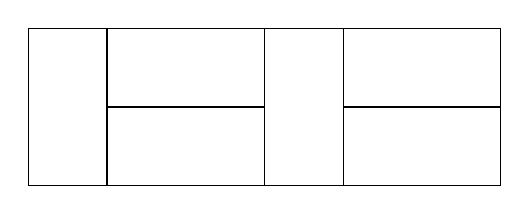
\begin{tikzpicture}
         \draw (0, 0) rectangle (6, 2);
         \draw (1, 0) rectangle (3, 1);
         \draw (1, 1) rectangle (3, 2);
         \draw (4, 0) rectangle (6, 1);
         \draw (4, 1) rectangle (6, 2);
        \end{tikzpicture}
      \end{center}
      We can do it recursively: suppose there are $f_n$ ways to tile a $2\times n$ grid. Then if we start tiling, the first tile is either vertical, in which we have $f_{n - 1}$ ways to tile the remaining ones; or the first tile is horizontal, in which we have $f_{n - 2}$ ways to tile the remaining. So
      \[
        f_n = f_{n - 1} + f_{n - 2},
      \]
      which is simply the Fibonacci sequence, with $f_0 = f_1 = 1$.
      Let
      \[
        F(z) = \sum_{n = 0}^\infty f_nz^n.
      \]
      Then from our recurrence relation, we obtain
      \[
        f_nz^n = f_{n - 1}z^n + f_{n - 2}z^n.
      \]
      So
      \[
        \sum_{n = 2}^\infty f_n z^n = \sum_{n = 2}^{\infty} f_{n - 1}z^n + \sum_{n = 2}^\infty f_{n - 2}z^n.
      \]
      Since $f_0 = f_1 = 1$, we have
      \[
        F(z) - f_0 - zf_1 = z(F(z) - f_0) + z^2F(z).
      \]
      Thus $F(z) = (1 - z - z^2)^{-1}$. If we write
      \[
        \alpha_1 = \frac{1}{2}(1 + \sqrt{5}),\quad \alpha_2 = \frac{1}{2}(1 - \sqrt{5}).
      \]
      then we have
      \begin{align*}
        F(z) &= (1 - z - z^2)^{-1}\\
        &= \frac{1}{(1 - \alpha_1 z)(1 - \alpha_2 z)}\\
        &= \frac{1}{\alpha_1 - \alpha_2}\left(\frac{\alpha_1}{1 - \alpha_1 z} - \frac{\alpha_2}{1 - \alpha_2 z}\right)\\
        &= \frac{1}{\alpha_1 - \alpha_2}\left(\alpha_1 \sum_{n = 0}^\infty \alpha_1^nz^n - \alpha_2\sum_{n = 0}^\infty \alpha_2^n z^n\right).
      \end{align*}
      So
      \[
        f_n = \frac{\alpha_1^{n + 1} - \alpha_2^{n + 1}}{\alpha_1 - \alpha_2}.
      \]
    \end{eg}
  \end{field}
  \begin{field}
    \begin{eg}
      Suppose we want to tile a $2\times n$ bathroom by $2\times 1$ tiles. One way to do it is
      \begin{center}
        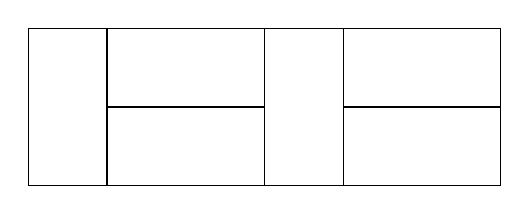
\begin{tikzpicture}
         \draw (0, 0) rectangle (6, 2);
         \draw (1, 0) rectangle (3, 1);
         \draw (1, 1) rectangle (3, 2);
         \draw (4, 0) rectangle (6, 1);
         \draw (4, 1) rectangle (6, 2);
        \end{tikzpicture}
      \end{center}
      We can do it recursively: suppose there are $f_n$ ways to tile a $2\times n$ grid. Then if we start tiling, the first tile is either vertical, in which we have $f_{n - 1}$ ways to tile the remaining ones; or the first tile is horizontal, in which we have $f_{n - 2}$ ways to tile the remaining. So
      \[
        f_n = f_{n - 1} + f_{n - 2},
      \]
      which is simply the Fibonacci sequence, with $f_0 = f_1 = 1$.
      Let
      \[
        F(z) = \sum_{n = 0}^\infty f_nz^n.
      \]
      Then from our recurrence relation, we obtain
      \[
        f_nz^n = f_{n - 1}z^n + f_{n - 2}z^n.
      \]
      So
      \[
        \sum_{n = 2}^\infty f_n z^n = \sum_{n = 2}^{\infty} f_{n - 1}z^n + \sum_{n = 2}^\infty f_{n - 2}z^n.
      \]
      Since $f_0 = f_1 = 1$, we have
      \[
        F(z) - f_0 - zf_1 = z(F(z) - f_0) + z^2F(z).
      \]
      Thus $F(z) = (1 - z - z^2)^{-1}$. If we write
      \[
        \alpha_1 = \frac{1}{2}(1 + \sqrt{5}),\quad \alpha_2 = \frac{1}{2}(1 - \sqrt{5}).
      \]
      then we have
      \begin{align*}
        F(z) &= (1 - z - z^2)^{-1}\\
        &= \frac{1}{(1 - \alpha_1 z)(1 - \alpha_2 z)}\\
        &= \frac{1}{\alpha_1 - \alpha_2}\left(\frac{\alpha_1}{1 - \alpha_1 z} - \frac{\alpha_2}{1 - \alpha_2 z}\right)\\
        &= \frac{1}{\alpha_1 - \alpha_2}\left(\alpha_1 \sum_{n = 0}^\infty \alpha_1^nz^n - \alpha_2\sum_{n = 0}^\infty \alpha_2^n z^n\right).
      \end{align*}
      So
      \[
        f_n = \frac{\alpha_1^{n + 1} - \alpha_2^{n + 1}}{\alpha_1 - \alpha_2}.
      \]
    \end{eg}
  \end{field}
  \xplain{3.5 Probability generating functions}% Subsection
  \xplain{3 Discrete random variables}% Section
  \xplain{}% Subject
  \xplain{GENERAL KNOWLEDGE}% Label
\end{note}

% To be manually edited
\begin{note}
  \xplain{probability.tex 147}
  \begin{field}
    \begin{eg}
      A \emph{Dyck word} is a string of brackets that match, such as (), or ((())()).
      There is only one Dyck word of length 2, (). There are 2 of length 4, (()) and ()(). Similarly, there are 5 Dyck words of length 5.
      Let $C_n$ be the number of Dyck words of length $2n$. We can split each Dyck word into $(w_1)w_2$, where $w_1$ and $w_2$ are Dyck words. Since the lengths of $w_1$ and $w_2$ must sum up to $2(n -1)$,
      \[
        C_{n + 1} = \sum_{i = 0}^n C_iC_{n - i}.\tag{$*$}
      \]
      We again use pgf-like functions: let
      \[
        c(x) = \sum_{n = 0}^\infty C_n x^n.
      \]
      From $(*)$, we can show that
      \[
        c(x) = 1 + xc(x)^2.
      \]
      We can solve to show that
      \[
        c(x) = \frac{1 - \sqrt{1 - 4x}}{2x} = \sum_0^\infty \binom{2n}{n}\frac{x^n}{n + 1},
      \]
      noting that $C_0 = 1$. Then
      \[
        C_n = \frac{1}{n + 1}\binom{2n}{n}.
      \]
    \end{eg}
  \end{field}
  \begin{field}
    \begin{eg}
      A \emph{Dyck word} is a string of brackets that match, such as (), or ((())()).
      There is only one Dyck word of length 2, (). There are 2 of length 4, (()) and ()(). Similarly, there are 5 Dyck words of length 5.
      Let $C_n$ be the number of Dyck words of length $2n$. We can split each Dyck word into $(w_1)w_2$, where $w_1$ and $w_2$ are Dyck words. Since the lengths of $w_1$ and $w_2$ must sum up to $2(n -1)$,
      \[
        C_{n + 1} = \sum_{i = 0}^n C_iC_{n - i}.\tag{$*$}
      \]
      We again use pgf-like functions: let
      \[
        c(x) = \sum_{n = 0}^\infty C_n x^n.
      \]
      From $(*)$, we can show that
      \[
        c(x) = 1 + xc(x)^2.
      \]
      We can solve to show that
      \[
        c(x) = \frac{1 - \sqrt{1 - 4x}}{2x} = \sum_0^\infty \binom{2n}{n}\frac{x^n}{n + 1},
      \]
      noting that $C_0 = 1$. Then
      \[
        C_n = \frac{1}{n + 1}\binom{2n}{n}.
      \]
    \end{eg}
  \end{field}
  \xplain{3.5 Probability generating functions}% Subsection
  \xplain{3 Discrete random variables}% Section
  \xplain{}% Subject
  \xplain{GENERAL KNOWLEDGE}% Label
\end{note}

% To be manually edited
\begin{note}
  \xplain{probability.tex 148}
  \begin{field}
    \begin{eg}
    Let $X_1, X_2, \cdots, X_n$ be iid with pgf $p(z) = \E[z^X]$. Let $N$ be a random variable independent of $X_i$ with pgf $h(z)$. What is the pgf of $S = X_1 + \cdots + X_N$?
    \begin{align*}
      \E[z^{S}] &= \E[z^{X_1 + \cdots + X_N}]\\
      &= \E_N[\underbrace{\E_{X_i}[z^{X_1 + \ldots + X_N}\mid N]}_{\text{assuming fixed }N}]\\
      &= \sum_{n = 0}^\infty \P(N = n) \E[z^{X_1 + X_2 + \cdots + X_n}]\\
      &= \sum_{n = 0}^\infty \P(N = n) \E[z^{X_1}] \E[z^{X_2}]\cdots\E[z^{X_n}]\\
      &= \sum_{n = 0}^\infty \P(N = n) (\E[z^{X_1}])^n\\
      &= \sum_{n = 0}^\infty \P(N = n) p(z)^n \\
      &= h(p(z))
    \end{align*}
    since $h(x) = \sum_{n = 0}^\infty \P(N = n) x^n$.
    So
    \begin{align*}
      \E[S] &= \left.\frac{\d }{\d z}h(p(z))\right|_{z = 1}\\
      &= h'(p(1))p'(1)\\
      &= \E[N]\E[X_1]
    \end{align*}
    To calculate the variance, use the fact that
    \[
      \E[S(S - 1)] = \left.\frac{\d ^2}{\d z^2}h(p(z))\right|_{z = 1}.
    \]
    Then we can find that
    \[
      \var (S) = \E[N]\var(X_1) + \E[X_1^2]\var(N).
    \]
    \end{eg}
  \end{field}
  \begin{field}
    \begin{eg}
    Let $X_1, X_2, \cdots, X_n$ be iid with pgf $p(z) = \E[z^X]$. Let $N$ be a random variable independent of $X_i$ with pgf $h(z)$. What is the pgf of $S = X_1 + \cdots + X_N$?
    \begin{align*}
      \E[z^{S}] &= \E[z^{X_1 + \cdots + X_N}]\\
      &= \E_N[\underbrace{\E_{X_i}[z^{X_1 + \ldots + X_N}\mid N]}_{\text{assuming fixed }N}]\\
      &= \sum_{n = 0}^\infty \P(N = n) \E[z^{X_1 + X_2 + \cdots + X_n}]\\
      &= \sum_{n = 0}^\infty \P(N = n) \E[z^{X_1}] \E[z^{X_2}]\cdots\E[z^{X_n}]\\
      &= \sum_{n = 0}^\infty \P(N = n) (\E[z^{X_1}])^n\\
      &= \sum_{n = 0}^\infty \P(N = n) p(z)^n \\
      &= h(p(z))
    \end{align*}
    since $h(x) = \sum_{n = 0}^\infty \P(N = n) x^n$.
    So
    \begin{align*}
      \E[S] &= \left.\frac{\d }{\d z}h(p(z))\right|_{z = 1}\\
      &= h'(p(1))p'(1)\\
      &= \E[N]\E[X_1]
    \end{align*}
    To calculate the variance, use the fact that
    \[
      \E[S(S - 1)] = \left.\frac{\d ^2}{\d z^2}h(p(z))\right|_{z = 1}.
    \]
    Then we can find that
    \[
      \var (S) = \E[N]\var(X_1) + \E[X_1^2]\var(N).
    \]
    \end{eg}
  \end{field}
  \xplain{3.5 Probability generating functions}% Subsection
  \xplain{3 Discrete random variables}% Section
  \xplain{}% Subject
  \xplain{GENERAL KNOWLEDGE}% Label
\end{note}

\section{Interesting problems}

\subsection{Branching processes}

% To be manually edited
\begin{note}
  \xplain{probability.tex 149}
  \begin{field}
    \begin{thm}
      \[
        F_{n + 1}(z) = F_n(F(z)) = F(F(F(\cdots F(z) \cdots )))) = F(F_n(z)).
      \]
    \end{thm}
  \end{field}
  \begin{field}
    \begin{thm}
      \[
        F_{n + 1}(z) = F_n(F(z)) = F(F(F(\cdots F(z) \cdots )))) = F(F_n(z)).
      \]
    \end{thm}
  \end{field}
  \xplain{4.1 Branching processes}% Subsection
  \xplain{4 Interesting problems}% Section
  \xplain{}% Subject
  \xplain{GENERAL KNOWLEDGE}% Label
\end{note}

%
\begin{note}
  \xplain{probability.tex 150}
  \begin{field}
    \begin{thm}
      \[
        F_{n + 1}(z) = F_n(F(z)) = F(F(F(\cdots F(z) \cdots )))) = F(F_n(z)).
      \]
    \end{thm}
  \end{field}
  \begin{field}
    \begin{proof}
      \begin{align*}
        F_{n + 1}(z) &= \E[z^{X_{n + 1}}]\\
        &= \E[\E[z^{X_{n + 1}}\mid X_n]]\\
        &= \sum_{k = 0}^\infty \P(X_n = k)\E[z^{X_{n + 1}}\mid X_n = k]\\
        &= \sum_{k = 0}^\infty \P(X_n = k)\E[z^{Y_1^n + \cdots + Y_k^n}\mid X_n = k]\\
        &= \sum_{k = 0}^\infty \P(X_n = k)\E[z^{Y_1}]\E[z^{Y_2}]\cdots\E[z^{Y_n}]\\
        &= \sum_{k = 0}^\infty \P(X_n = k)(\E[z^{X_1}])^k\\
        &= \sum_{k = 0}\P(X_n = k)F(z)^k\\
        &= F_n(F(z))
      \end{align*}
    \end{proof}
  \end{field}
  \xplain{4.1 Branching processes}% Subsection
  \xplain{4 Interesting problems}% Section
  \xplain{}% Subject
  \xplain{PROOF EXERCISE}% Label
\end{note}

% To be manually edited
\begin{note}
  \xplain{probability.tex 151}
  \begin{field}
    \begin{thm}
      Suppose
      \[
        \E[X_1] = \sum k p_k = \mu
      \]
      and
      \[
        \var (X_1) = \E[(X - \mu)^2] = \sum (k - \mu)^2 p_k < \infty.
      \]
      Then
      \[
        \E[X_n] = \mu^n,\quad \var X_n = \sigma^2\mu^{n - 1}(1 + \mu + \mu^2 + \cdots + \mu^{n - 1}).
      \]
    \end{thm}
  \end{field}
  \begin{field}
    \begin{thm}
      Suppose
      \[
        \E[X_1] = \sum k p_k = \mu
      \]
      and
      \[
        \var (X_1) = \E[(X - \mu)^2] = \sum (k - \mu)^2 p_k < \infty.
      \]
      Then
      \[
        \E[X_n] = \mu^n,\quad \var X_n = \sigma^2\mu^{n - 1}(1 + \mu + \mu^2 + \cdots + \mu^{n - 1}).
      \]
    \end{thm}
  \end{field}
  \xplain{4.1 Branching processes}% Subsection
  \xplain{4 Interesting problems}% Section
  \xplain{}% Subject
  \xplain{GENERAL KNOWLEDGE}% Label
\end{note}

%
\begin{note}
  \xplain{probability.tex 152}
  \begin{field}
    \begin{thm}
      Suppose
      \[
        \E[X_1] = \sum k p_k = \mu
      \]
      and
      \[
        \var (X_1) = \E[(X - \mu)^2] = \sum (k - \mu)^2 p_k < \infty.
      \]
      Then
      \[
        \E[X_n] = \mu^n,\quad \var X_n = \sigma^2\mu^{n - 1}(1 + \mu + \mu^2 + \cdots + \mu^{n - 1}).
      \]
    \end{thm}
  \end{field}
  \begin{field}
    \begin{proof}
    \begin{align*}
      \E[X_n] &= \E[\E[X_n\mid X_{n - 1}]]\\
      &= \E[\mu X_{n - 1}]\\
      &= \mu \E[X_{n - 1}]
    \end{align*}
    Then by induction, $\E[X_n] = \mu^n$ (since $X_0 = 1$).
    To calculate the variance, note that
    \[
      \var (X_n) = \E[X_n^2] - (\E[X_n])^2
    \]
    and hence
    \[
      \E[X_n^2] = \var(X_n) + (\E[X])^2
    \]
    We then calculate
    \begin{align*}
      \E[X_n^2] &= \E[\E[X_n^2\mid X_{n - 1}]]\\
      &= \E[\var(X_n) + (\E[X_n])^2 \mid X_{n - 1}]\\
      &= \E[X_{n - 1}\var (X_1) + (\mu X_{n - 1})^2]\\
      &= \E[X_{n - 1}\sigma^2 + (\mu X_{n - 1})^2]\\
      &= \sigma^2 \mu^{n - 1} + \mu^2 \E[X_{n - 1}^2].
    \end{align*}
    So
    \begin{align*}
      \var X_n &= \E[X_n^2] - (\E[X_n])^2 \\
      &= \mu^2 \E[X_{n -1}^2] + \sigma^2 \mu^{n - 1} - \mu^2 (\E[X_{n - 1}])^2\\
      &= \mu^2(\E[X_{n - 1}^2] - \E[X_{n - 1}]^2) + \sigma^2\mu^{n - 1}\\
      &= \mu^2 \var (X_{n - 1}) + \sigma^2 \mu^{n -1 }\\
      &= \mu^4 \var(X_{n - 2}) + \sigma^2(\mu^{n - 1} + \mu^n)\\
      &= \cdots\\
      &= \mu^{2(n - 1)}\var (X_1) + \sigma^2 (\mu^{n - 1} + \mu^{n} + \cdots + \mu^{2n - 3})\\
      &= \sigma^2\mu^{n - 1}(1 + \mu + \cdots + \mu^{n - 1}).
    \end{align*}
    Of course, we can also obtain this using the probability generating function as well.
    \end{proof}
  \end{field}
  \xplain{4.1 Branching processes}% Subsection
  \xplain{4 Interesting problems}% Section
  \xplain{}% Subject
  \xplain{PROOF EXERCISE}% Label
\end{note}

% To be manually edited
\begin{note}
  \xplain{probability.tex 153}
  \begin{field}
    \begin{thm}
      The probability of extinction $q$ is the smallest root to the equation $q = F(q)$. Write $\mu = \E[X_1]$. Then if $\mu \leq 1$, then $q = 1$; if $\mu > 1$, then $q < 1$.
    \end{thm}
  \end{field}
  \begin{field}
    \begin{thm}
      The probability of extinction $q$ is the smallest root to the equation $q = F(q)$. Write $\mu = \E[X_1]$. Then if $\mu \leq 1$, then $q = 1$; if $\mu > 1$, then $q < 1$.
    \end{thm}
  \end{field}
  \xplain{4.1 Branching processes}% Subsection
  \xplain{4 Interesting problems}% Section
  \xplain{}% Subject
  \xplain{GENERAL KNOWLEDGE}% Label
\end{note}

%
\begin{note}
  \xplain{probability.tex 154}
  \begin{field}
    \begin{thm}
      The probability of extinction $q$ is the smallest root to the equation $q = F(q)$. Write $\mu = \E[X_1]$. Then if $\mu \leq 1$, then $q = 1$; if $\mu > 1$, then $q < 1$.
    \end{thm}
  \end{field}
  \begin{field}
    \begin{proof}
      To show that it is the smallest root, let $\alpha$ be the smallest root. Then note that $0 \leq \alpha \Rightarrow F(0) \leq F(\alpha) = \alpha$ since $F$ is increasing (proof: write the function out!). Hence $F(F(0)) \leq \alpha$. Continuing inductively, $F_n(0) \leq \alpha$ for all $n$. So
      \[
        q = \lim_{n \to \infty}F_n(0) \leq \alpha.
      \]
      So $q = \alpha$.
      To show that $q = 1$ when $\mu \leq 1$, we show that $q = 1$ is the only root. We know that $F'(z), F''(z) \geq 0$ for $z\in (0, 1)$ (proof: write it out again!). So $F$ is increasing and convex. Since $F'(1) = \mu \leq 1$, it must approach $(1, 1)$ from above the $F = z$ line. So it must look like this:
      \begin{center}
        \begin{tikzpicture}
          \draw (0, 0) -- (4, 0) node [right] {$z$};
          \draw (0, 0) -- (0, 4) node [above] {$F(z)$};
          \draw [dashed] (0, 0) -- (4, 4);
          \draw (0, 2.3) parabola (4, 4);
        \end{tikzpicture}
      \end{center}
      So $z = 1$ is the only root.
    \end{proof}
  \end{field}
  \xplain{4.1 Branching processes}% Subsection
  \xplain{4 Interesting problems}% Section
  \xplain{}% Subject
  \xplain{PROOF EXERCISE}% Label
\end{note}

\subsection{Random walk and gambler's ruin}

%
\begin{note}
  \xplain{probability.tex 155}
  \begin{field}
    Random walk
  \end{field}
  \begin{field}
    \begin{defi}[Random walk]
      Let $X_1, \cdots, X_n$ be iid random variables such that $X_n = +1$ with probability $p$, and $-1$ with probability $1 - p$. Let $S_n = S_0 + X_1 + \cdots + X_n$. Then $(S_0, S_1, \cdots, S_n)$ is a \emph{1-dimensional random walk}.
      If $p = q = \frac{1}{2}$, we say it is a \emph{symmetric random walk}.
    \end{defi}
  \end{field}
  \xplain{4.2 Random walk and gambler's ruin}% Subsection
  \xplain{4 Interesting problems}% Section
  \xplain{}% Subject
  \xplain{VOCABULARY}% Label
\end{note}

% To be manually edited
\begin{note}
  \xplain{probability.tex 156}
  \begin{field}
    \begin{eg}
      A gambler starts with $\$z$, with $z < a$, and plays a game in which he wins $\$1$ or loses $\$ 1$ at each turn with probabilities $p$ and $q$ respectively. What are
      \[
        p_z = \P(\text{random walk hits $a$ before } 0 \mid \text{starts at } z),
      \]
      and
      \[
        q_z = \P(\text{random walk hits 0 before }a \mid \text{starts at }z)?
      \]
      He either wins his first game, with probability $p$, or loses with probability $q$. So
      \[
        p_z = qp_{z - 1} + pp_{z + 1},
      \]
      for $0 < z < a$, and $p_0 = 0, p_a = 1$.
      Try $p_z = t^z$. Then
      \[
        pt^2 - t + q = (pt - q)(t - 1) = 0,
      \]
      noting that $p = 1 - q$. If $p \not = q$, then
      \[
        p_z = A1^z + B\left(\frac{q}{p}\right)^z.
      \]
      Since $p_0 = 0$, we get $A = -B$. Since $p_a = 1$, we obtain
      \[
        p_z = \frac{1 - (q/p)^z}{1 - (q/p)^a}.
      \]
      If $p = q$, then $p_z = A + Bz = z/a$.
      Similarly, (or perform the substitutions $p\mapsto q$, $q\mapsto p$ and $z \mapsto a - z$)
      \[
        q_z = \frac{(q/p)^a - (q/p)^z}{(q / p)^a - 1}
      \]
      if $p\not = q$, and
      \[
        q_z = \frac{a - z}{a}
      \]
      if $p = q$. Since $p_z + q_z = 1$, we know that the game will eventually end.
      What if $a\to \infty$? What is the probability of going bankrupt?
      \begin{align*}
        \P(\text{path hits 0 ever}) &= \P\left(\bigcup_{a = z+1}^\infty [\text{path hits 0 before }a]\right)\\
        &= \lim_{a\to \infty}\P(\text{path hits 0 before }a)\\
        &= \lim_{a\to \infty}q_z\\
        &= \begin{cases}
          (q/p)^z & p > q\\
          1 & p \leq q.
        \end{cases}
      \end{align*}
      So if the odds are against you (i.e.\ the probability of losing is greater than the probability of winning), then no matter how small the difference is, you are bound to going bankrupt eventually.
    \end{eg}
  \end{field}
  \begin{field}
    \begin{eg}
      A gambler starts with $\$z$, with $z < a$, and plays a game in which he wins $\$1$ or loses $\$ 1$ at each turn with probabilities $p$ and $q$ respectively. What are
      \[
        p_z = \P(\text{random walk hits $a$ before } 0 \mid \text{starts at } z),
      \]
      and
      \[
        q_z = \P(\text{random walk hits 0 before }a \mid \text{starts at }z)?
      \]
      He either wins his first game, with probability $p$, or loses with probability $q$. So
      \[
        p_z = qp_{z - 1} + pp_{z + 1},
      \]
      for $0 < z < a$, and $p_0 = 0, p_a = 1$.
      Try $p_z = t^z$. Then
      \[
        pt^2 - t + q = (pt - q)(t - 1) = 0,
      \]
      noting that $p = 1 - q$. If $p \not = q$, then
      \[
        p_z = A1^z + B\left(\frac{q}{p}\right)^z.
      \]
      Since $p_0 = 0$, we get $A = -B$. Since $p_a = 1$, we obtain
      \[
        p_z = \frac{1 - (q/p)^z}{1 - (q/p)^a}.
      \]
      If $p = q$, then $p_z = A + Bz = z/a$.
      Similarly, (or perform the substitutions $p\mapsto q$, $q\mapsto p$ and $z \mapsto a - z$)
      \[
        q_z = \frac{(q/p)^a - (q/p)^z}{(q / p)^a - 1}
      \]
      if $p\not = q$, and
      \[
        q_z = \frac{a - z}{a}
      \]
      if $p = q$. Since $p_z + q_z = 1$, we know that the game will eventually end.
      What if $a\to \infty$? What is the probability of going bankrupt?
      \begin{align*}
        \P(\text{path hits 0 ever}) &= \P\left(\bigcup_{a = z+1}^\infty [\text{path hits 0 before }a]\right)\\
        &= \lim_{a\to \infty}\P(\text{path hits 0 before }a)\\
        &= \lim_{a\to \infty}q_z\\
        &= \begin{cases}
          (q/p)^z & p > q\\
          1 & p \leq q.
        \end{cases}
      \end{align*}
      So if the odds are against you (i.e.\ the probability of losing is greater than the probability of winning), then no matter how small the difference is, you are bound to going bankrupt eventually.
    \end{eg}
  \end{field}
  \xplain{4.2 Random walk and gambler's ruin}% Subsection
  \xplain{4 Interesting problems}% Section
  \xplain{}% Subject
  \xplain{GENERAL KNOWLEDGE}% Label
\end{note}

\section{Continuous random variables}

\subsection{Continuous random variables}

% To be manually edited
\begin{note}
  \xplain{probability.tex 157}
  \begin{field}
    \begin{defi}[Continuous random variable]
      A random variable $X : \Omega \to \R$ is \emph{continuous} if there is a function $f : \R \to \R_{\geq 0}$ such that
      \[
        \P(a \leq X \leq b) = \int_a^b f(x) \;\d x.
      \]
      We call $f$ the \emph{probability density function}, which satisfies
      \begin{itemize}
        \item $f \geq 0$
        \item $\int_{-\infty}^\infty f(x) = 1$.
      \end{itemize}
    \end{defi}
  \end{field}
  \begin{field}
    \begin{defi}[Continuous random variable]
      A random variable $X : \Omega \to \R$ is \emph{continuous} if there is a function $f : \R \to \R_{\geq 0}$ such that
      \[
        \P(a \leq X \leq b) = \int_a^b f(x) \;\d x.
      \]
      We call $f$ the \emph{probability density function}, which satisfies
      \begin{itemize}
        \item $f \geq 0$
        \item $\int_{-\infty}^\infty f(x) = 1$.
      \end{itemize}
    \end{defi}
  \end{field}
  \xplain{5.1 Continuous random variables}% Subsection
  \xplain{5 Continuous random variables}% Section
  \xplain{}% Subject
  \xplain{VOCABULARY}% Label
\end{note}

%
\begin{note}
  \xplain{probability.tex 158}
  \begin{field}
    Cumulative distribution function
  \end{field}
  \begin{field}
    \begin{defi}[Cumulative distribution function]
      The \emph{cumulative distribution function} (or simply \emph{distribution function}) of a random variable $X$ (discrete, continuous, or neither) is
      \[
        F(x) = \P(X \leq x).
      \]
    \end{defi}
  \end{field}
  \xplain{5.1 Continuous random variables}% Subsection
  \xplain{5 Continuous random variables}% Section
  \xplain{}% Subject
  \xplain{VOCABULARY}% Label
\end{note}

% To be manually edited
\begin{note}
  \xplain{probability.tex 159}
  \begin{field}
    \begin{defi}[Uniform distribution]
      The \emph{uniform distribution} on $[a, b]$ has pdf
      \[
        f(x) = \frac{1}{b - a}.
      \]
      Then
      \[
        F(x) = \int_a^x f(z)\;\d z = \frac{x - a}{b - a}
      \]
      for $a \leq x \leq b$.
      If $X$ follows a uniform distribution on $[a, b]$, we write $X\sim U[a, b]$.
    \end{defi}
  \end{field}
  \begin{field}
    \begin{defi}[Uniform distribution]
      The \emph{uniform distribution} on $[a, b]$ has pdf
      \[
        f(x) = \frac{1}{b - a}.
      \]
      Then
      \[
        F(x) = \int_a^x f(z)\;\d z = \frac{x - a}{b - a}
      \]
      for $a \leq x \leq b$.
      If $X$ follows a uniform distribution on $[a, b]$, we write $X\sim U[a, b]$.
    \end{defi}
  \end{field}
  \xplain{5.1 Continuous random variables}% Subsection
  \xplain{5 Continuous random variables}% Section
  \xplain{}% Subject
  \xplain{VOCABULARY}% Label
\end{note}

% To be manually edited
\begin{note}
  \xplain{probability.tex 160}
  \begin{field}
    \begin{defi}[Exponential random variable]
      The \emph{exponential random variable with parameter $\lambda$} has pdf
      \[
        f(x) = \lambda e^{-\lambda x}
      \]
      and
      \[
        F(x) = 1 - e^{-\lambda x}
      \]
      for $x \geq 0$.
      We write $X \sim \mathcal{E}(\lambda)$.
    \end{defi}
  \end{field}
  \begin{field}
    \begin{defi}[Exponential random variable]
      The \emph{exponential random variable with parameter $\lambda$} has pdf
      \[
        f(x) = \lambda e^{-\lambda x}
      \]
      and
      \[
        F(x) = 1 - e^{-\lambda x}
      \]
      for $x \geq 0$.
      We write $X \sim \mathcal{E}(\lambda)$.
    \end{defi}
  \end{field}
  \xplain{5.1 Continuous random variables}% Subsection
  \xplain{5 Continuous random variables}% Section
  \xplain{}% Subject
  \xplain{VOCABULARY}% Label
\end{note}

% To be manually edited
\begin{note}
  \xplain{probability.tex 161}
  \begin{field}
    \begin{prop}
      The exponential random variable is \emph{memoryless}, i.e.
      \[
        \P(X \geq x + z \mid X \geq x) = \P(X \geq z).
      \]
      This means that, say if $X$ measures the lifetime of a light bulb, knowing it has already lasted for 3 hours does not give any information about how much longer it will last.
    \end{prop}
  \end{field}
  \begin{field}
    \begin{prop}
      The exponential random variable is \emph{memoryless}, i.e.
      \[
        \P(X \geq x + z \mid X \geq x) = \P(X \geq z).
      \]
      This means that, say if $X$ measures the lifetime of a light bulb, knowing it has already lasted for 3 hours does not give any information about how much longer it will last.
    \end{prop}
  \end{field}
  \xplain{5.1 Continuous random variables}% Subsection
  \xplain{5 Continuous random variables}% Section
  \xplain{}% Subject
  \xplain{GENERAL KNOWLEDGE}% Label
\end{note}

%
\begin{note}
  \xplain{probability.tex 162}
  \begin{field}
    \begin{prop}
      The exponential random variable is \emph{memoryless}, i.e.
      \[
        \P(X \geq x + z \mid X \geq x) = \P(X \geq z).
      \]
      This means that, say if $X$ measures the lifetime of a light bulb, knowing it has already lasted for 3 hours does not give any information about how much longer it will last.
    \end{prop}
  \end{field}
  \begin{field}
    \begin{proof}
      \begin{align*}
        \P(X \geq x + z \mid X \geq x) &= \frac{\P(X \geq x + z)}{\P(X \geq x)}\\
        &= \frac{\int_{x + z}^\infty f(u)\;\d u}{\int_x^\infty f(u)\;\d u}\\
        &= \frac{e^{-\lambda(x + z)}}{e^{-\lambda x}}\\
        &= e^{-\lambda z}\\
        &= \P(X \geq z).\qedhere
      \end{align*}
    \end{proof}
  \end{field}
  \xplain{5.1 Continuous random variables}% Subsection
  \xplain{5 Continuous random variables}% Section
  \xplain{}% Subject
  \xplain{PROOF EXERCISE}% Label
\end{note}

%
\begin{note}
  \xplain{probability.tex 163}
  \begin{field}
    Expectation
  \end{field}
  \begin{field}
    \begin{defi}[Expectation]
      The \emph{expectation} (or \emph{mean}) of a continuous random variable is
      \[
        \E[X] = \int_{-\infty}^\infty xf(x) \;\d x,
      \]
      provided not both $\int_0^\infty xf(x)\;\d x$ and $\int_{-\infty}^0 xf(x) \;\d x$ are infinite.
    \end{defi}
  \end{field}
  \xplain{5.1 Continuous random variables}% Subsection
  \xplain{5 Continuous random variables}% Section
  \xplain{}% Subject
  \xplain{VOCABULARY}% Label
\end{note}

% To be manually edited
\begin{note}
  \xplain{probability.tex 164}
  \begin{field}
    \begin{thm}
      If $X$ is a continuous random variable, then
      \[
        \E[X] = \int_0^\infty \P(X \geq x)\;\d x - \int_0^\infty \P(X \leq -x)\;\d x.
      \]
    \end{thm}
  \end{field}
  \begin{field}
    \begin{thm}
      If $X$ is a continuous random variable, then
      \[
        \E[X] = \int_0^\infty \P(X \geq x)\;\d x - \int_0^\infty \P(X \leq -x)\;\d x.
      \]
    \end{thm}
  \end{field}
  \xplain{5.1 Continuous random variables}% Subsection
  \xplain{5 Continuous random variables}% Section
  \xplain{}% Subject
  \xplain{GENERAL KNOWLEDGE}% Label
\end{note}

%
\begin{note}
  \xplain{probability.tex 165}
  \begin{field}
    \begin{thm}
      If $X$ is a continuous random variable, then
      \[
        \E[X] = \int_0^\infty \P(X \geq x)\;\d x - \int_0^\infty \P(X \leq -x)\;\d x.
      \]
    \end{thm}
  \end{field}
  \begin{field}
    \begin{proof}
      \begin{align*}
        \int_0^\infty \P(X \geq x)\;\d x &= \int_0^\infty \int_x^\infty f(y)\;\d y\;\d x\\
        &= \int_0^\infty \int_0^\infty I[y\geq x]f(y)\;\d y\;\d x\\
        &= \int_0^\infty \left(\int_0^\infty I[x\leq y]\;\d x\right) f(y)\;\d y\\
        &= \int_0^\infty yf(y)\;\d y.
      \end{align*}
      We can similarly show that $\int_0^\infty \P(X \leq -x)\;\d x = -\int_{-\infty}^0 yf(y)\;\d y$.
    \end{proof}
  \end{field}
  \xplain{5.1 Continuous random variables}% Subsection
  \xplain{5 Continuous random variables}% Section
  \xplain{}% Subject
  \xplain{PROOF EXERCISE}% Label
\end{note}

% To be manually edited
\begin{note}
  \xplain{probability.tex 166}
  \begin{field}
    \begin{eg}
      Suppose $X\sim \mathcal{E}(\lambda)$. Then
      \[
        \P(X \geq x) = \int_x^{\infty} \lambda e^{-\lambda t}\;\d t = e^{-\lambda x}.
      \]
      So
      \[
        \E[X] = \int_0^\infty e^{-\lambda x}\;\d x = \frac{1}{\lambda}.\qedhere
      \]
    \end{eg}
  \end{field}
  \begin{field}
    \begin{eg}
      Suppose $X\sim \mathcal{E}(\lambda)$. Then
      \[
        \P(X \geq x) = \int_x^{\infty} \lambda e^{-\lambda t}\;\d t = e^{-\lambda x}.
      \]
      So
      \[
        \E[X] = \int_0^\infty e^{-\lambda x}\;\d x = \frac{1}{\lambda}.\qedhere
      \]
    \end{eg}
  \end{field}
  \xplain{5.1 Continuous random variables}% Subsection
  \xplain{5 Continuous random variables}% Section
  \xplain{}% Subject
  \xplain{GENERAL KNOWLEDGE}% Label
\end{note}

%
\begin{note}
  \xplain{probability.tex 167}
  \begin{field}
    Variance
  \end{field}
  \begin{field}
    \begin{defi}[Variance]
      The \emph{variance} of a continuous random variable is
      \[
        \var (X) = \E[(X - \E[X])^2] = \E[X^2] - (E[X])^2.
      \]
    \end{defi}
  \end{field}
  \xplain{5.1 Continuous random variables}% Subsection
  \xplain{5 Continuous random variables}% Section
  \xplain{}% Subject
  \xplain{VOCABULARY}% Label
\end{note}

% To be manually edited
\begin{note}
  \xplain{probability.tex 168}
  \begin{field}
    \begin{eg}
      Let $X\sim U[a, b]$. Then
      \[
        \E[X] = \int_a^b x\frac{1}{b - a}\;d x = \frac{a + b}{2}.
      \]
      So
      \begin{align*}
        \var (X) &= \int_a^b x^2\frac{1}{b - a}\;\d x - (\E[X])^2\\
        &= \frac{1}{12}(b - a)^2.
      \end{align*}
    \end{eg}
  \end{field}
  \begin{field}
    \begin{eg}
      Let $X\sim U[a, b]$. Then
      \[
        \E[X] = \int_a^b x\frac{1}{b - a}\;d x = \frac{a + b}{2}.
      \]
      So
      \begin{align*}
        \var (X) &= \int_a^b x^2\frac{1}{b - a}\;\d x - (\E[X])^2\\
        &= \frac{1}{12}(b - a)^2.
      \end{align*}
    \end{eg}
  \end{field}
  \xplain{5.1 Continuous random variables}% Subsection
  \xplain{5 Continuous random variables}% Section
  \xplain{}% Subject
  \xplain{GENERAL KNOWLEDGE}% Label
\end{note}

% To be manually edited
\begin{note}
  \xplain{probability.tex 169}
  \begin{field}
    \begin{defi}[Mode and median]
      Given a pdf $f(x)$, we call $\hat x$ a \emph{mode} if
      \[
        f(\hat x) \geq f(x)
      \]
      for all $x$. Note that a distribution can have many modes. For example, in the uniform distribution, all $x$ are modes.
      We say it is a median if
      \[
        \int_{-\infty}^{\hat x}f(x)\;\d x = \frac{1}{2} = \int_{\hat x}^\infty f(x)\;\d x.
      \]
      For a discrete random variable, the median is $\hat x$ such that
      \[
        \P(X \leq \hat x) \geq \frac{1}{2}, \quad \P(X \geq \hat x) \geq \frac{1}{2}.
      \]
      Here we have a non-strict inequality since if the random variable, say, always takes value $0$, then both probabilities will be 1.
    \end{defi}
  \end{field}
  \begin{field}
    \begin{defi}[Mode and median]
      Given a pdf $f(x)$, we call $\hat x$ a \emph{mode} if
      \[
        f(\hat x) \geq f(x)
      \]
      for all $x$. Note that a distribution can have many modes. For example, in the uniform distribution, all $x$ are modes.
      We say it is a median if
      \[
        \int_{-\infty}^{\hat x}f(x)\;\d x = \frac{1}{2} = \int_{\hat x}^\infty f(x)\;\d x.
      \]
      For a discrete random variable, the median is $\hat x$ such that
      \[
        \P(X \leq \hat x) \geq \frac{1}{2}, \quad \P(X \geq \hat x) \geq \frac{1}{2}.
      \]
      Here we have a non-strict inequality since if the random variable, say, always takes value $0$, then both probabilities will be 1.
    \end{defi}
  \end{field}
  \xplain{5.1 Continuous random variables}% Subsection
  \xplain{5 Continuous random variables}% Section
  \xplain{}% Subject
  \xplain{VOCABULARY}% Label
\end{note}

%
\begin{note}
  \xplain{probability.tex 170}
  \begin{field}
    Sample mean
  \end{field}
  \begin{field}
    \begin{defi}[Sample mean]
      If $X_1, \cdots, X_n$ is a random sample from some distribution, then the \emph{sample mean} is
      \[
        \bar X = \frac{1}{n}\sum_1^n X_i.
      \]
    \end{defi}
  \end{field}
  \xplain{5.1 Continuous random variables}% Subsection
  \xplain{5 Continuous random variables}% Section
  \xplain{}% Subject
  \xplain{VOCABULARY}% Label
\end{note}

\subsection{Stochastic ordering and inspection paradox}

%
\begin{note}
  \xplain{probability.tex 171}
  \begin{field}
    Stochastic order
  \end{field}
  \begin{field}
    \begin{defi}[Stochastic order]
      The \emph{stochastic order} is defined as: $X \geq_{\mathrm{st}} Y$ if $\P(X > t) \geq \P(Y > t)$ for all $t$.
    \end{defi}
  \end{field}
  \xplain{5.2 Stochastic ordering and inspection paradox}% Subsection
  \xplain{5 Continuous random variables}% Section
  \xplain{}% Subject
  \xplain{VOCABULARY}% Label
\end{note}

% To be manually edited
\begin{note}
  \xplain{probability.tex 172}
  \begin{field}
    \begin{eg}[Inspection paradox]
      Suppose that $n$ families have children attending a school. Family $i$ has $X_i$ children at the school, where $X_1, \cdots, X_n$ are iid random variables, with $P(X_i = k) = p_k$. Suppose that the average family size is $\mu$.
      Now pick a child at random. What is the probability distribution of his family size? Let $J$ be the index of the family from which she comes (which is a random variable). Then
      \[
        \P(X_J = k\mid J = j) = \frac{\P(J = j, X_j = k)}{\P(J = j)}.
      \]
      The denominator is $1/n$. The numerator is more complex. This would require the $j$th family to have $k$ members, which happens with probability $p_k$; and that we picked a member from the $j$th family, which happens with probability $\E\left[\frac{k}{k + \sum_{i \not=j} X_i}\right]$. So
      \[
        \P(X_J = k \mid J = j) = \E\left[\frac{nkp_k}{k + \sum_{i \not=j} X_i}\right].
      \]
      Note that this is independent of $j$. So
      \[
        \P(X_J = k) = \E\left[\frac{nkp_k}{k + \sum_{i \not=j} X_i}\right].
      \]
      Also, $\P(X_1 = k) = p_k$. So
      \[
        \frac{\P(X_J = k)}{\P(X_1 = k)} = \E\left[\frac{nk}{k + \sum_{i \not= j}X_i}\right].
      \]
      This is increasing in $k$, and greater than $1$ for $k > \mu$. So the average value of the family size of the child we picked is greater than the average family size. It can be shown that $X_J$ is stochastically greater than $X_1$.
      This means that if we pick the children randomly, the sample mean of the family size will be greater than the actual mean. This is since for the larger a family is, the more likely it is for us to pick a child from the family.
    \end{eg}
  \end{field}
  \begin{field}
    \begin{eg}[Inspection paradox]
      Suppose that $n$ families have children attending a school. Family $i$ has $X_i$ children at the school, where $X_1, \cdots, X_n$ are iid random variables, with $P(X_i = k) = p_k$. Suppose that the average family size is $\mu$.
      Now pick a child at random. What is the probability distribution of his family size? Let $J$ be the index of the family from which she comes (which is a random variable). Then
      \[
        \P(X_J = k\mid J = j) = \frac{\P(J = j, X_j = k)}{\P(J = j)}.
      \]
      The denominator is $1/n$. The numerator is more complex. This would require the $j$th family to have $k$ members, which happens with probability $p_k$; and that we picked a member from the $j$th family, which happens with probability $\E\left[\frac{k}{k + \sum_{i \not=j} X_i}\right]$. So
      \[
        \P(X_J = k \mid J = j) = \E\left[\frac{nkp_k}{k + \sum_{i \not=j} X_i}\right].
      \]
      Note that this is independent of $j$. So
      \[
        \P(X_J = k) = \E\left[\frac{nkp_k}{k + \sum_{i \not=j} X_i}\right].
      \]
      Also, $\P(X_1 = k) = p_k$. So
      \[
        \frac{\P(X_J = k)}{\P(X_1 = k)} = \E\left[\frac{nk}{k + \sum_{i \not= j}X_i}\right].
      \]
      This is increasing in $k$, and greater than $1$ for $k > \mu$. So the average value of the family size of the child we picked is greater than the average family size. It can be shown that $X_J$ is stochastically greater than $X_1$.
      This means that if we pick the children randomly, the sample mean of the family size will be greater than the actual mean. This is since for the larger a family is, the more likely it is for us to pick a child from the family.
    \end{eg}
  \end{field}
  \xplain{5.2 Stochastic ordering and inspection paradox}% Subsection
  \xplain{5 Continuous random variables}% Section
  \xplain{}% Subject
  \xplain{GENERAL KNOWLEDGE}% Label
\end{note}

\subsection{Jointly distributed random variables}

%
\begin{note}
  \xplain{probability.tex 173}
  \begin{field}
    Joint distribution
  \end{field}
  \begin{field}
    \begin{defi}[Joint distribution]
      Two random variables $X, Y$ have \emph{joint distribution} $F: \R^2 \mapsto [0, 1]$ defined by
      \[
        F(x, y) = \P(X \leq x, Y \leq y).
      \]
      The \emph{marginal distribution} of $X$ is
      \[
        F_X(x) = \P(X \leq x) = \P(X \leq x, Y < \infty) = F(x, \infty) = \lim_{y \to \infty}F(x, y)
      \]
    \end{defi}
  \end{field}
  \xplain{5.3 Jointly distributed random variables}% Subsection
  \xplain{5 Continuous random variables}% Section
  \xplain{}% Subject
  \xplain{VOCABULARY}% Label
\end{note}

% To be manually edited
\begin{note}
  \xplain{probability.tex 174}
  \begin{field}
    \begin{defi}[Jointly distributed random variables]
      We say $X_1, \cdots, X_n$ are \emph{jointly distributed continuous random variables} and have \emph{joint pdf} $f$ if for any set $A\subseteq \R^n$
      \[
        \P((X_1, \cdots, X_n)\in A) = \int_{(x_1, \cdots x_n)\in A} f(x_1, \cdots, x_n)\;\d x_1\cdots \d x_n.
      \]
      where
      \[
        f(x_1, \cdots, x_n) \geq 0
      \]
      and
      \[
        \int_{\R^n} f(x_1, \cdots, x_n)\;\d x_1 \cdots \d x_n = 1.
      \]
    \end{defi}
  \end{field}
  \begin{field}
    \begin{defi}[Jointly distributed random variables]
      We say $X_1, \cdots, X_n$ are \emph{jointly distributed continuous random variables} and have \emph{joint pdf} $f$ if for any set $A\subseteq \R^n$
      \[
        \P((X_1, \cdots, X_n)\in A) = \int_{(x_1, \cdots x_n)\in A} f(x_1, \cdots, x_n)\;\d x_1\cdots \d x_n.
      \]
      where
      \[
        f(x_1, \cdots, x_n) \geq 0
      \]
      and
      \[
        \int_{\R^n} f(x_1, \cdots, x_n)\;\d x_1 \cdots \d x_n = 1.
      \]
    \end{defi}
  \end{field}
  \xplain{5.3 Jointly distributed random variables}% Subsection
  \xplain{5 Continuous random variables}% Section
  \xplain{}% Subject
  \xplain{VOCABULARY}% Label
\end{note}

% To be manually edited
\begin{note}
  \xplain{probability.tex 175}
  \begin{field}
    \begin{eg}
      In the case where $n = 2$,
      \[
        F(x, y) = \P(X \leq x,Y \leq y) = \int_{-\infty}^x\int_{-\infty}^y f(x, y)\;\d x\;\d y.
      \]
      If $F$ is differentiable, then
      \[
        f(x, y) = \frac{\partial^2}{\partial x\partial y}F(x, y).
      \]
    \end{eg}
  \end{field}
  \begin{field}
    \begin{eg}
      In the case where $n = 2$,
      \[
        F(x, y) = \P(X \leq x,Y \leq y) = \int_{-\infty}^x\int_{-\infty}^y f(x, y)\;\d x\;\d y.
      \]
      If $F$ is differentiable, then
      \[
        f(x, y) = \frac{\partial^2}{\partial x\partial y}F(x, y).
      \]
    \end{eg}
  \end{field}
  \xplain{5.3 Jointly distributed random variables}% Subsection
  \xplain{5 Continuous random variables}% Section
  \xplain{}% Subject
  \xplain{GENERAL KNOWLEDGE}% Label
\end{note}

% To be manually edited
\begin{note}
  \xplain{probability.tex 176}
  \begin{field}
    \begin{thm}
      If $X$ and $Y$ are jointly continuous random variables, then they are individually continuous random variables.
    \end{thm}
  \end{field}
  \begin{field}
    \begin{thm}
      If $X$ and $Y$ are jointly continuous random variables, then they are individually continuous random variables.
    \end{thm}
  \end{field}
  \xplain{5.3 Jointly distributed random variables}% Subsection
  \xplain{5 Continuous random variables}% Section
  \xplain{}% Subject
  \xplain{GENERAL KNOWLEDGE}% Label
\end{note}

%
\begin{note}
  \xplain{probability.tex 177}
  \begin{field}
    \begin{thm}
      If $X$ and $Y$ are jointly continuous random variables, then they are individually continuous random variables.
    \end{thm}
  \end{field}
  \begin{field}
    \begin{proof}
      We prove this by showing that $X$ has a density function.
      We know that
      \begin{align*}
        \P(X \in A) &= \P(X \in A, Y\in (-\infty, +\infty))\\
        &= \int_{x\in A}\int_{-\infty}^\infty f(x, y)\;\d y\;\d x\\
        &= \int_{x\in A} f_X(x)\;\d x
      \end{align*}
      So
      \[
        f_X(x) = \int_{-\infty}^\infty f(x, y)\;\d y
      \]
      is the (marginal) pdf of $X$.
    \end{proof}
  \end{field}
  \xplain{5.3 Jointly distributed random variables}% Subsection
  \xplain{5 Continuous random variables}% Section
  \xplain{}% Subject
  \xplain{PROOF EXERCISE}% Label
\end{note}

% To be manually edited
\begin{note}
  \xplain{probability.tex 178}
  \begin{field}
    \begin{defi}[Independent continuous random variables]
      Continuous random variables $X_1, \cdots, X_n$ are independent if
      \[
        \P(X_1\in A_1, X_2 \in A_2, \cdots, X_n\in A_n) = \P(X_1 \in A_1)\P(X_2 \in A_2) \cdots \P(X_n \in A_n)
      \]
      for all $A_i\subseteq \Omega_{X_i}$.
      If we let $F_{X_i}$ and $f_{X_i}$ be the cdf, pdf of $X$, then
      \[
        F(x_1, \cdots, x_n) = F_{X_1}(x_1)\cdots F_{X_n}(x_n)
      \]
      and
      \[
        f(x_1, \cdots, x_n) = f_{X_1}(x_1) \cdots f_{X_n}(x_n)
      \]
      are each individually equivalent to the definition above.
    \end{defi}
  \end{field}
  \begin{field}
    \begin{defi}[Independent continuous random variables]
      Continuous random variables $X_1, \cdots, X_n$ are independent if
      \[
        \P(X_1\in A_1, X_2 \in A_2, \cdots, X_n\in A_n) = \P(X_1 \in A_1)\P(X_2 \in A_2) \cdots \P(X_n \in A_n)
      \]
      for all $A_i\subseteq \Omega_{X_i}$.
      If we let $F_{X_i}$ and $f_{X_i}$ be the cdf, pdf of $X$, then
      \[
        F(x_1, \cdots, x_n) = F_{X_1}(x_1)\cdots F_{X_n}(x_n)
      \]
      and
      \[
        f(x_1, \cdots, x_n) = f_{X_1}(x_1) \cdots f_{X_n}(x_n)
      \]
      are each individually equivalent to the definition above.
    \end{defi}
  \end{field}
  \xplain{5.3 Jointly distributed random variables}% Subsection
  \xplain{5 Continuous random variables}% Section
  \xplain{}% Subject
  \xplain{VOCABULARY}% Label
\end{note}

% To be manually edited
\begin{note}
  \xplain{probability.tex 179}
  \begin{field}
    \begin{eg}
      If $(X_1, X_2)$ takes a random value from $[0, 1] \times [0, 1]$, then $f(x_1, x_2) = 1$. Then we can see that $f(x_1, x_2) = 1\cdot 1 = f(x_1)\cdot f(x_2)$. So $X_1$ and $X_2$ are independent.
      On the other hand, if $(Y_1, Y_2)$ takes a random value from $[0, 1] \times [0, 1]$ with the restriction that $Y_1 \leq Y_2$, then they are not independent, since $f(x_1, x_2) = 2 I[Y_1 \leq Y_2]$, which cannot be split into two parts.
    \end{eg}
  \end{field}
  \begin{field}
    \begin{eg}
      If $(X_1, X_2)$ takes a random value from $[0, 1] \times [0, 1]$, then $f(x_1, x_2) = 1$. Then we can see that $f(x_1, x_2) = 1\cdot 1 = f(x_1)\cdot f(x_2)$. So $X_1$ and $X_2$ are independent.
      On the other hand, if $(Y_1, Y_2)$ takes a random value from $[0, 1] \times [0, 1]$ with the restriction that $Y_1 \leq Y_2$, then they are not independent, since $f(x_1, x_2) = 2 I[Y_1 \leq Y_2]$, which cannot be split into two parts.
    \end{eg}
  \end{field}
  \xplain{5.3 Jointly distributed random variables}% Subsection
  \xplain{5 Continuous random variables}% Section
  \xplain{}% Subject
  \xplain{GENERAL KNOWLEDGE}% Label
\end{note}

% To be manually edited
\begin{note}
  \xplain{probability.tex 180}
  \begin{field}
    \begin{prop}
      For independent continuous random variables $X_i$,
      \begin{enumerate}
        \item $\E [\prod X_i] = \prod \E [X_i]$
        \item $\var (\sum X_i) = \sum \var (X_i)$
      \end{enumerate}
    \end{prop}
  \end{field}
  \begin{field}
    \begin{prop}
      For independent continuous random variables $X_i$,
      \begin{enumerate}
        \item $\E [\prod X_i] = \prod \E [X_i]$
        \item $\var (\sum X_i) = \sum \var (X_i)$
      \end{enumerate}
    \end{prop}
  \end{field}
  \xplain{5.3 Jointly distributed random variables}% Subsection
  \xplain{5 Continuous random variables}% Section
  \xplain{}% Subject
  \xplain{GENERAL KNOWLEDGE}% Label
\end{note}

\subsection{Geometric probability}

% To be manually edited
\begin{note}
  \xplain{probability.tex 181}
  \begin{field}
    \begin{eg}
      Two points $X$ and $Y$ are chosen independently on a line segment of length $L$. What is the probability that $|X - Y| \leq \ell$? By ``at random'', we mean
      \[
        f(x, y) = \frac{1}{L^2},
      \]
      since each of $X$ and $Y$ have pdf $1/L$.
      We can visualize this on a graph:
      \begin{center}
        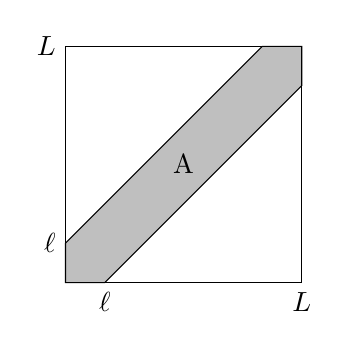
\begin{tikzpicture}
          \draw (0, 0) rectangle (3, 3);
          \draw [fill=gray!50!white] (0, 0) -- (0.5, 0) -- (3, 2.5) -- (3, 3) -- (2.5, 3) -- (0, 0.5) -- cycle;
          \node at (1.5, 1.5) {A};
          \node at (0.5, 0) [below] {$\ell$};
          \node at (3, 0) [below] {$L$};
          \node at (0, 0.5) [left] {$\ell$};
          \node at (0, 3) [left] {$L$};
        \end{tikzpicture}
      \end{center}
      Here the two axes are the values of $X$ and $Y$, and $A$ is the permitted region. The total area of the white part is simply the area of a square with length $L - \ell$. So the area of $A$ is $L^2 - (L - \ell)^2 = 2L\ell - \ell^2$. So the desired probability is
      \[
        \int_A f(x, y)\;\d x\;\d y = \frac{2L\ell - \ell^2}{L^2}.
      \]
    \end{eg}
  \end{field}
  \begin{field}
    \begin{eg}
      Two points $X$ and $Y$ are chosen independently on a line segment of length $L$. What is the probability that $|X - Y| \leq \ell$? By ``at random'', we mean
      \[
        f(x, y) = \frac{1}{L^2},
      \]
      since each of $X$ and $Y$ have pdf $1/L$.
      We can visualize this on a graph:
      \begin{center}
        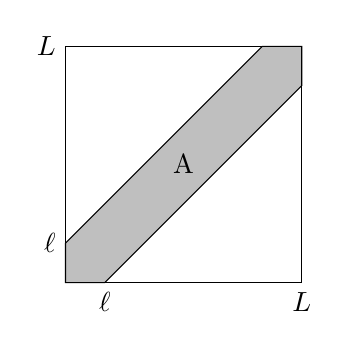
\begin{tikzpicture}
          \draw (0, 0) rectangle (3, 3);
          \draw [fill=gray!50!white] (0, 0) -- (0.5, 0) -- (3, 2.5) -- (3, 3) -- (2.5, 3) -- (0, 0.5) -- cycle;
          \node at (1.5, 1.5) {A};
          \node at (0.5, 0) [below] {$\ell$};
          \node at (3, 0) [below] {$L$};
          \node at (0, 0.5) [left] {$\ell$};
          \node at (0, 3) [left] {$L$};
        \end{tikzpicture}
      \end{center}
      Here the two axes are the values of $X$ and $Y$, and $A$ is the permitted region. The total area of the white part is simply the area of a square with length $L - \ell$. So the area of $A$ is $L^2 - (L - \ell)^2 = 2L\ell - \ell^2$. So the desired probability is
      \[
        \int_A f(x, y)\;\d x\;\d y = \frac{2L\ell - \ell^2}{L^2}.
      \]
    \end{eg}
  \end{field}
  \xplain{5.4 Geometric probability}% Subsection
  \xplain{5 Continuous random variables}% Section
  \xplain{}% Subject
  \xplain{GENERAL KNOWLEDGE}% Label
\end{note}

% To be manually edited
\begin{note}
  \xplain{probability.tex 182}
  \begin{field}
    \begin{eg}[Bertrand's paradox]
      Suppose we draw a random chord in a circle. What is the probability that the length of the chord is greater than the length of the side of an inscribed equilateral triangle?
      There are three ways of ``drawing a random chord''.
      \begin{enumerate}
        \item We randomly pick two end points over the circumference independently. Now draw the inscribed triangle with the vertex at one end point. For the length of the chord to be longer than a side of the triangle, the other end point must between the two other vertices of the triangle. This happens with probability $1/3$.
          \begin{center}
            \begin{tikzpicture}
              \draw circle [radius = 1];
              \draw (0, 1) -- (0.866, -0.5) -- (-0.866, -0.5) -- cycle;
              \node [circ, fill=red] at (0, 1) {};
              \draw [mblue] (0, 1) -- (-1, 0);
              \draw [mred] (0, 1) -- (0, -1);
              \draw [mblue] (0, 1) -- (1, 0);
            \end{tikzpicture}
          \end{center}
        \item wlog the chord is horizontal, on the lower side of the circle. The mid-point is uniformly distributed along the middle (dashed) line. Then the probability of getting a long line is $1/2$.
          \begin{center}
            \begin{tikzpicture}
              \draw circle [radius = 1];
              \draw (0, 1) -- (0.866, -0.5) -- (-0.866, -0.5) -- cycle;
              \node [circ, fill=mred] at (0, 1) {};
              \draw [dashed] (0, 1) -- (0, -1);
              \draw [mblue] (-0.4359, -0.9) -- (0.4359, -0.9);
              \draw [mblue] (-0.8, -0.6) -- (0.8, -0.6);
              \draw [mred] (-0.9539, -0.3) -- (0.9539, -0.3);
              \draw [mred] (-1, 0) -- (1, 0);
            \end{tikzpicture}
          \end{center}
        \item The mid point of the chord is distributed uniformly across the circle. Then you get a long line if and only if the mid-point lies in the smaller circle shown below. This occurs with probability $1/4$.
           \begin{center}
            \begin{tikzpicture}
              \draw circle [radius = 1];
              \draw (0, 1) -- (0.866, -0.5) -- (-0.866, -0.5) -- cycle;
              \node [circ, fill=mred] at (0, 1) {};
              \draw circle [radius = 0.5];
              \draw [mred] (0, -1) -- (-0.6, 0.8);
              \draw [mblue] (-0.9539, 0.3) -- (0.4359, 0.9);
              \draw [mblue] (0.6, -0.8) -- (0.9165, 0.4);
              \draw [mblue] (-1, 0) -- (0.3, -0.9539);
            \end{tikzpicture}
          \end{center}
      \end{enumerate}
      We get different answers for different notions of ``random''! This is why when we say ``randomly'', we should be explicit in what we mean by that.
    \end{eg}
  \end{field}
  \begin{field}
    \begin{eg}[Bertrand's paradox]
      Suppose we draw a random chord in a circle. What is the probability that the length of the chord is greater than the length of the side of an inscribed equilateral triangle?
      There are three ways of ``drawing a random chord''.
      \begin{enumerate}
        \item We randomly pick two end points over the circumference independently. Now draw the inscribed triangle with the vertex at one end point. For the length of the chord to be longer than a side of the triangle, the other end point must between the two other vertices of the triangle. This happens with probability $1/3$.
          \begin{center}
            \begin{tikzpicture}
              \draw circle [radius = 1];
              \draw (0, 1) -- (0.866, -0.5) -- (-0.866, -0.5) -- cycle;
              \node [circ, fill=red] at (0, 1) {};
              \draw [mblue] (0, 1) -- (-1, 0);
              \draw [mred] (0, 1) -- (0, -1);
              \draw [mblue] (0, 1) -- (1, 0);
            \end{tikzpicture}
          \end{center}
        \item wlog the chord is horizontal, on the lower side of the circle. The mid-point is uniformly distributed along the middle (dashed) line. Then the probability of getting a long line is $1/2$.
          \begin{center}
            \begin{tikzpicture}
              \draw circle [radius = 1];
              \draw (0, 1) -- (0.866, -0.5) -- (-0.866, -0.5) -- cycle;
              \node [circ, fill=mred] at (0, 1) {};
              \draw [dashed] (0, 1) -- (0, -1);
              \draw [mblue] (-0.4359, -0.9) -- (0.4359, -0.9);
              \draw [mblue] (-0.8, -0.6) -- (0.8, -0.6);
              \draw [mred] (-0.9539, -0.3) -- (0.9539, -0.3);
              \draw [mred] (-1, 0) -- (1, 0);
            \end{tikzpicture}
          \end{center}
        \item The mid point of the chord is distributed uniformly across the circle. Then you get a long line if and only if the mid-point lies in the smaller circle shown below. This occurs with probability $1/4$.
           \begin{center}
            \begin{tikzpicture}
              \draw circle [radius = 1];
              \draw (0, 1) -- (0.866, -0.5) -- (-0.866, -0.5) -- cycle;
              \node [circ, fill=mred] at (0, 1) {};
              \draw circle [radius = 0.5];
              \draw [mred] (0, -1) -- (-0.6, 0.8);
              \draw [mblue] (-0.9539, 0.3) -- (0.4359, 0.9);
              \draw [mblue] (0.6, -0.8) -- (0.9165, 0.4);
              \draw [mblue] (-1, 0) -- (0.3, -0.9539);
            \end{tikzpicture}
          \end{center}
      \end{enumerate}
      We get different answers for different notions of ``random''! This is why when we say ``randomly'', we should be explicit in what we mean by that.
    \end{eg}
  \end{field}
  \xplain{5.4 Geometric probability}% Subsection
  \xplain{5 Continuous random variables}% Section
  \xplain{}% Subject
  \xplain{GENERAL KNOWLEDGE}% Label
\end{note}

% To be manually edited
\begin{note}
  \xplain{probability.tex 183}
  \begin{field}
    \begin{eg}[Buffon's needle]
      A needle of length $\ell$ is tossed at random onto a floor marked with parallel lines a distance $L$ apart, where $\ell \leq L$. Let $A$ be the event that the needle intersects a line. What is $\P(A)$?
      \begin{center}
        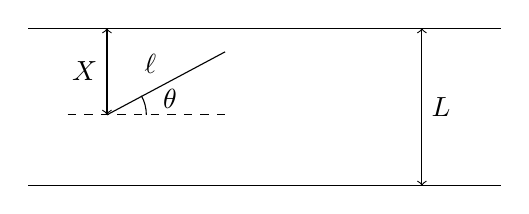
\begin{tikzpicture}
          \draw (-3, -1) -- (3, -1);
          \draw (-3, 1) -- (3, 1);
          \draw (-2, -0.1) -- (-0.5, 0.7) node [anchor = south east, pos = 0.5] {$\ell$};
          \draw [->] (-2, -0.1) -- (-2, 1) node [left, pos = 0.5] {$X$};
          \draw [->] (-2, 1) -- (-2, -0.1);
          \draw [dashed] (-2.5, -0.1) -- (-0.5, -0.1);
          \draw (-1.5, -0.1) arc (0:29:0.5);
          \node at (-1.2, 0.1) {$\theta$};
          \draw [->] (2, -1) -- (2, 1) node [right, pos = 0.5] {$L$};
          \draw [->] (2, 1) -- (2, -1);
        \end{tikzpicture}
      \end{center}
      Suppose that $X\sim U[0, L]$ and $\theta\sim U[0, \pi]$. Then
      \[
        f(x, \theta) = \frac{1}{L\pi}.
      \]
      This touches a line iff $X \leq \ell \sin \theta$. Hence
      \[
        \P(A) = \int_{\theta = 0}^\pi \underbrace{\frac{\ell \sin \theta}{L}}_{\P(X \leq \ell\sin \theta)}\frac{1}{\pi}\d \theta = \frac{2\ell }{\pi L}.
      \]
      Since the answer involves $\pi$, we can estimate $\pi$ by conducting repeated experiments! Suppose we have $N$ hits out of $n$ tosses. Then an estimator for $p$ is $\hat{p} = \frac{N}{n}$. Hence
      \[
        \hat{\pi} = \frac{2\ell}{\hat{p}L}.
      \]
      We will later find out that this is a really inefficient way of estimating $\pi$ (as you could have guessed).
    \end{eg}
  \end{field}
  \begin{field}
    \begin{eg}[Buffon's needle]
      A needle of length $\ell$ is tossed at random onto a floor marked with parallel lines a distance $L$ apart, where $\ell \leq L$. Let $A$ be the event that the needle intersects a line. What is $\P(A)$?
      \begin{center}
        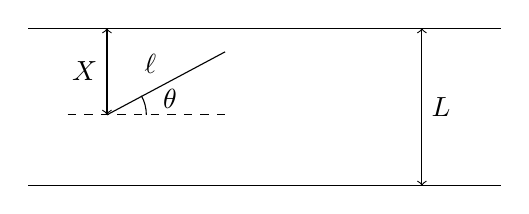
\begin{tikzpicture}
          \draw (-3, -1) -- (3, -1);
          \draw (-3, 1) -- (3, 1);
          \draw (-2, -0.1) -- (-0.5, 0.7) node [anchor = south east, pos = 0.5] {$\ell$};
          \draw [->] (-2, -0.1) -- (-2, 1) node [left, pos = 0.5] {$X$};
          \draw [->] (-2, 1) -- (-2, -0.1);
          \draw [dashed] (-2.5, -0.1) -- (-0.5, -0.1);
          \draw (-1.5, -0.1) arc (0:29:0.5);
          \node at (-1.2, 0.1) {$\theta$};
          \draw [->] (2, -1) -- (2, 1) node [right, pos = 0.5] {$L$};
          \draw [->] (2, 1) -- (2, -1);
        \end{tikzpicture}
      \end{center}
      Suppose that $X\sim U[0, L]$ and $\theta\sim U[0, \pi]$. Then
      \[
        f(x, \theta) = \frac{1}{L\pi}.
      \]
      This touches a line iff $X \leq \ell \sin \theta$. Hence
      \[
        \P(A) = \int_{\theta = 0}^\pi \underbrace{\frac{\ell \sin \theta}{L}}_{\P(X \leq \ell\sin \theta)}\frac{1}{\pi}\d \theta = \frac{2\ell }{\pi L}.
      \]
      Since the answer involves $\pi$, we can estimate $\pi$ by conducting repeated experiments! Suppose we have $N$ hits out of $n$ tosses. Then an estimator for $p$ is $\hat{p} = \frac{N}{n}$. Hence
      \[
        \hat{\pi} = \frac{2\ell}{\hat{p}L}.
      \]
      We will later find out that this is a really inefficient way of estimating $\pi$ (as you could have guessed).
    \end{eg}
  \end{field}
  \xplain{5.4 Geometric probability}% Subsection
  \xplain{5 Continuous random variables}% Section
  \xplain{}% Subject
  \xplain{GENERAL KNOWLEDGE}% Label
\end{note}

\subsection{The normal distribution}

% To be manually edited
\begin{note}
  \xplain{probability.tex 184}
  \begin{field}
    \begin{defi}[Normal distribution]
      The \emph{normal distribution} with parameters $\mu, \sigma^2$, written $N(\mu, \sigma^2)$ has pdf
      \[
        f(x) = \frac{1}{\sqrt{2 \pi}\sigma}\exp\left(-\frac{(x - \mu)^2}{2\sigma^2}\right),
      \]
      for $-\infty < x < \infty$.
      It looks approximately like this:
      \begin{center}
        \begin{tikzpicture}[yscale=1.5]
          \draw (-3, 0) -- (3, 0);
          \draw (0, 1.3) -- (0, 0) node [below] {$\mu$};
          \draw [domain=-3:3,samples=50, mblue] plot (\x, {exp(-\x * \x)});
        \end{tikzpicture}
      \end{center}
      The \emph{standard normal} is when $\mu = 0, \sigma^2 = 1$, i.e.\ $X\sim N(0, 1)$.
      We usually write $\phi(x)$ for the pdf and $\Phi(x)$ for the cdf of the standard normal.
    \end{defi}
  \end{field}
  \begin{field}
    \begin{defi}[Normal distribution]
      The \emph{normal distribution} with parameters $\mu, \sigma^2$, written $N(\mu, \sigma^2)$ has pdf
      \[
        f(x) = \frac{1}{\sqrt{2 \pi}\sigma}\exp\left(-\frac{(x - \mu)^2}{2\sigma^2}\right),
      \]
      for $-\infty < x < \infty$.
      It looks approximately like this:
      \begin{center}
        \begin{tikzpicture}[yscale=1.5]
          \draw (-3, 0) -- (3, 0);
          \draw (0, 1.3) -- (0, 0) node [below] {$\mu$};
          \draw [domain=-3:3,samples=50, mblue] plot (\x, {exp(-\x * \x)});
        \end{tikzpicture}
      \end{center}
      The \emph{standard normal} is when $\mu = 0, \sigma^2 = 1$, i.e.\ $X\sim N(0, 1)$.
      We usually write $\phi(x)$ for the pdf and $\Phi(x)$ for the cdf of the standard normal.
    \end{defi}
  \end{field}
  \xplain{5.5 The normal distribution}% Subsection
  \xplain{5 Continuous random variables}% Section
  \xplain{}% Subject
  \xplain{VOCABULARY}% Label
\end{note}

% To be manually edited
\begin{note}
  \xplain{probability.tex 185}
  \begin{field}
    \begin{prop}
      \[
        \int_{-\infty}^\infty \frac{1}{\sqrt{2\pi \sigma^2}} e^{-\frac{1}{2\sigma^2}(x - \mu)^2}\;\d x = 1.
      \]
    \end{prop}
  \end{field}
  \begin{field}
    \begin{prop}
      \[
        \int_{-\infty}^\infty \frac{1}{\sqrt{2\pi \sigma^2}} e^{-\frac{1}{2\sigma^2}(x - \mu)^2}\;\d x = 1.
      \]
    \end{prop}
  \end{field}
  \xplain{5.5 The normal distribution}% Subsection
  \xplain{5 Continuous random variables}% Section
  \xplain{}% Subject
  \xplain{GENERAL KNOWLEDGE}% Label
\end{note}

%
\begin{note}
  \xplain{probability.tex 186}
  \begin{field}
    \begin{prop}
      \[
        \int_{-\infty}^\infty \frac{1}{\sqrt{2\pi \sigma^2}} e^{-\frac{1}{2\sigma^2}(x - \mu)^2}\;\d x = 1.
      \]
    \end{prop}
  \end{field}
  \begin{field}
    \begin{proof}
      Substitute $z = \frac{(x - \mu)}{\sigma}$. Then
      \[
        I = \int_{-\infty}^\infty \frac{1}{\sqrt{2\pi}}e^{-\frac{1}{2}z^2}\;\d z.
      \]
      Then
      \begin{align*}
        I^2 &= \int_{-\infty}^\infty \frac{1}{\sqrt{2\pi}} e^{-x^2/2}\;\d x\int_{\infty}^\infty \frac{1}{\sqrt{2\pi}} e^{-y^2/2}\;\d y\\
        &= \int_0^\infty \int_0^{2\pi}\frac{1}{2\pi}e^{-r^2/2}r\;\d r\;\d \theta\\
        &= 1.\qedhere
      \end{align*}
    \end{proof}
  \end{field}
  \xplain{5.5 The normal distribution}% Subsection
  \xplain{5 Continuous random variables}% Section
  \xplain{}% Subject
  \xplain{PROOF EXERCISE}% Label
\end{note}

% To be manually edited
\begin{note}
  \xplain{probability.tex 187}
  \begin{field}
    \begin{prop}
      $\E[X] = \mu$.
    \end{prop}
  \end{field}
  \begin{field}
    \begin{prop}
      $\E[X] = \mu$.
    \end{prop}
  \end{field}
  \xplain{5.5 The normal distribution}% Subsection
  \xplain{5 Continuous random variables}% Section
  \xplain{}% Subject
  \xplain{GENERAL KNOWLEDGE}% Label
\end{note}

%
\begin{note}
  \xplain{probability.tex 188}
  \begin{field}
    \begin{prop}
      $\E[X] = \mu$.
    \end{prop}
  \end{field}
  \begin{field}
    \begin{proof}
    \begin{align*}
      \E[X] &= \frac{1}{\sqrt{2\pi}\sigma} \int_{-\infty}^\infty x e^{-(x - \mu)^2/2\sigma^2}\;\d x\\
      &= \frac{1}{\sqrt{2\pi} \sigma}\int_{-\infty}^\infty (x - \mu)e^{-(x - \mu)^2/2\sigma^2}\;\d x + \frac{1}{\sqrt{2\pi}\sigma}\int_{-\infty}^\infty \mu e^{-(x - \mu)^2/2\sigma^2}\;\d x.
    \end{align*}
    The first term is antisymmetric about $\mu$ and gives $0$. The second is just $\mu$ times the integral we did above. So we get $\mu$.
    \end{proof}
  \end{field}
  \xplain{5.5 The normal distribution}% Subsection
  \xplain{5 Continuous random variables}% Section
  \xplain{}% Subject
  \xplain{PROOF EXERCISE}% Label
\end{note}

% To be manually edited
\begin{note}
  \xplain{probability.tex 189}
  \begin{field}
    \begin{prop}
      $\var(X) = \sigma^2$.
    \end{prop}
  \end{field}
  \begin{field}
    \begin{prop}
      $\var(X) = \sigma^2$.
    \end{prop}
  \end{field}
  \xplain{5.5 The normal distribution}% Subsection
  \xplain{5 Continuous random variables}% Section
  \xplain{}% Subject
  \xplain{GENERAL KNOWLEDGE}% Label
\end{note}

%
\begin{note}
  \xplain{probability.tex 190}
  \begin{field}
    \begin{prop}
      $\var(X) = \sigma^2$.
    \end{prop}
  \end{field}
  \begin{field}
    \begin{proof}
      We have $\var (X) = \E[X^2] - (\E[X])^2$. Substitute $Z = \frac{X - \mu}{\sigma}$. Then $\E[Z] = 0$, $\E[Z^2] = \frac{1}{\sigma^2}\E[X^2]$.
      Then
      \begin{align*}
        \var(Z) &= \frac{1}{\sqrt{2\pi}} \int_{-\infty}^\infty z^2 e^{-z^2/2}\;\d z\\
        &= \left[-\frac{1}{\sqrt{2\pi}}ze^{-z^2/2}\right]_{-\infty}^\infty + \frac{1}{\sqrt{2\pi}}\int_{-\infty}^\infty e^{-z^2/2}\;\d z\\
        &= 0 + 1\\
        &= 1
      \end{align*}
      So $\var X = \sigma^2$.
    \end{proof}
  \end{field}
  \xplain{5.5 The normal distribution}% Subsection
  \xplain{5 Continuous random variables}% Section
  \xplain{}% Subject
  \xplain{PROOF EXERCISE}% Label
\end{note}

% To be manually edited
\begin{note}
  \xplain{probability.tex 191}
  \begin{field}
    \begin{eg}
      UK adult male heights are normally distributed with mean 70'' and standard deviation 3''. In the Netherlands, these figures are 71'' and 3''.
      What is $\P(Y > X)$, where $X$ and $Y$ are the heights of randomly chosen UK and Netherlands males, respectively?
      We have $X\sim N(70, 3^2)$ and $Y\sim N(71, 3^2)$. Then (as we will show in later lectures) $Y - X \sim N(1, 18)$.
      \[
        \P(Y > X) = \P(Y - X > 0) = \P\left(\frac{Y - X - 1}{\sqrt{18}} > \frac{-1}{\sqrt{18}}\right) = 1 - \Phi(-1/\sqrt{18}),
      \]
      since $\frac{(Y - X) - 1}{\sqrt{18}}\sim N(0, 1)$, and the answer is approximately 0.5931.
      Now suppose that in both countries, the Olympic male basketball teams are selected from that portion of male whose hight is at least above 4'' above the mean (which corresponds to the $9.1\%$ tallest males of the country). What is the probability that a randomly chosen Netherlands player is taller than a randomly chosen UK player?
      For the second part, we have
      \[
        \P(Y > X\mid X \geq 74, Y \geq 75) = \frac{\int_{x = 74}^{75} \phi_X(x)\;\d x + \int_{x = 75}^\infty \int_{y=x}^\infty \phi_Y(y)\phi_X(x)\;\d y\;\d x}{\int_{x=74}^\infty \phi_X(x)\;\d x \int_{y=75}^\infty \phi_Y(y)\;\d y},
      \]
      which is approximately 0.7558. So even though the Netherlands people are only slightly taller, if we consider the tallest bunch, the Netherlands people will be much taller on average.
    \end{eg}
  \end{field}
  \begin{field}
    \begin{eg}
      UK adult male heights are normally distributed with mean 70'' and standard deviation 3''. In the Netherlands, these figures are 71'' and 3''.
      What is $\P(Y > X)$, where $X$ and $Y$ are the heights of randomly chosen UK and Netherlands males, respectively?
      We have $X\sim N(70, 3^2)$ and $Y\sim N(71, 3^2)$. Then (as we will show in later lectures) $Y - X \sim N(1, 18)$.
      \[
        \P(Y > X) = \P(Y - X > 0) = \P\left(\frac{Y - X - 1}{\sqrt{18}} > \frac{-1}{\sqrt{18}}\right) = 1 - \Phi(-1/\sqrt{18}),
      \]
      since $\frac{(Y - X) - 1}{\sqrt{18}}\sim N(0, 1)$, and the answer is approximately 0.5931.
      Now suppose that in both countries, the Olympic male basketball teams are selected from that portion of male whose hight is at least above 4'' above the mean (which corresponds to the $9.1\%$ tallest males of the country). What is the probability that a randomly chosen Netherlands player is taller than a randomly chosen UK player?
      For the second part, we have
      \[
        \P(Y > X\mid X \geq 74, Y \geq 75) = \frac{\int_{x = 74}^{75} \phi_X(x)\;\d x + \int_{x = 75}^\infty \int_{y=x}^\infty \phi_Y(y)\phi_X(x)\;\d y\;\d x}{\int_{x=74}^\infty \phi_X(x)\;\d x \int_{y=75}^\infty \phi_Y(y)\;\d y},
      \]
      which is approximately 0.7558. So even though the Netherlands people are only slightly taller, if we consider the tallest bunch, the Netherlands people will be much taller on average.
    \end{eg}
  \end{field}
  \xplain{5.5 The normal distribution}% Subsection
  \xplain{5 Continuous random variables}% Section
  \xplain{}% Subject
  \xplain{GENERAL KNOWLEDGE}% Label
\end{note}

\subsection{Transformation of random variables}

% To be manually edited
\begin{note}
  \xplain{probability.tex 192}
  \begin{field}
    \begin{thm}
      If $X$ is a continuous random variable with a pdf $f(x)$, and $h(x)$ is a continuous, strictly increasing function with $h^{-1}(x)$ differentiable, then $Y = h(X)$ is a random variable with pdf
      \[
        f_Y(y) = f_X(h^{-1}(y))\frac{\d }{\d y}h^{-1}(y).
      \]
    \end{thm}
  \end{field}
  \begin{field}
    \begin{thm}
      If $X$ is a continuous random variable with a pdf $f(x)$, and $h(x)$ is a continuous, strictly increasing function with $h^{-1}(x)$ differentiable, then $Y = h(X)$ is a random variable with pdf
      \[
        f_Y(y) = f_X(h^{-1}(y))\frac{\d }{\d y}h^{-1}(y).
      \]
    \end{thm}
  \end{field}
  \xplain{5.6 Transformation of random variables}% Subsection
  \xplain{5 Continuous random variables}% Section
  \xplain{}% Subject
  \xplain{GENERAL KNOWLEDGE}% Label
\end{note}

%
\begin{note}
  \xplain{probability.tex 193}
  \begin{field}
    \begin{thm}
      If $X$ is a continuous random variable with a pdf $f(x)$, and $h(x)$ is a continuous, strictly increasing function with $h^{-1}(x)$ differentiable, then $Y = h(X)$ is a random variable with pdf
      \[
        f_Y(y) = f_X(h^{-1}(y))\frac{\d }{\d y}h^{-1}(y).
      \]
    \end{thm}
  \end{field}
  \begin{field}
    \begin{proof}
      \begin{align*}
        F_Y(y) &= \P(Y \leq y)\\
        &= \P(h(X) \leq y)\\
        &= \P(X \leq h^{-1}(y))\\
        &= F(h^{-1}(y))
      \end{align*}
      Take the derivative with respect to $y$ to obtain
      \[
        f_Y(y) = F'_Y(y) = f(h^{-1}(y))\frac{\d}{\d y}h^{-1}(y).\qedhere
      \]
    \end{proof}
  \end{field}
  \xplain{5.6 Transformation of random variables}% Subsection
  \xplain{5 Continuous random variables}% Section
  \xplain{}% Subject
  \xplain{PROOF EXERCISE}% Label
\end{note}

% To be manually edited
\begin{note}
  \xplain{probability.tex 194}
  \begin{field}
    \begin{eg}
      Let $X\sim U[0, 1]$. Let $Y = -\log X$. Then
      \begin{align*}
        \P(Y \leq y) &= \P(-\log X \leq y)\\
        &= \P(X \geq e^{-y})\\
        &= 1 - e^{-y}.
      \end{align*}
      But this is the cumulative distribution function of $\mathcal{E}(1)$. So $Y$ is exponentially distributed with $\lambda = 1$.
    \end{eg}
  \end{field}
  \begin{field}
    \begin{eg}
      Let $X\sim U[0, 1]$. Let $Y = -\log X$. Then
      \begin{align*}
        \P(Y \leq y) &= \P(-\log X \leq y)\\
        &= \P(X \geq e^{-y})\\
        &= 1 - e^{-y}.
      \end{align*}
      But this is the cumulative distribution function of $\mathcal{E}(1)$. So $Y$ is exponentially distributed with $\lambda = 1$.
    \end{eg}
  \end{field}
  \xplain{5.6 Transformation of random variables}% Subsection
  \xplain{5 Continuous random variables}% Section
  \xplain{}% Subject
  \xplain{GENERAL KNOWLEDGE}% Label
\end{note}

% To be manually edited
\begin{note}
  \xplain{probability.tex 195}
  \begin{field}
    \begin{thm}
      Let $U\sim U[0, 1]$. For any strictly increasing distribution function $F$, the random variable $X = F^{-1}U$ has distribution function $F$.
    \end{thm}
  \end{field}
  \begin{field}
    \begin{thm}
      Let $U\sim U[0, 1]$. For any strictly increasing distribution function $F$, the random variable $X = F^{-1}U$ has distribution function $F$.
    \end{thm}
  \end{field}
  \xplain{5.6 Transformation of random variables}% Subsection
  \xplain{5 Continuous random variables}% Section
  \xplain{}% Subject
  \xplain{GENERAL KNOWLEDGE}% Label
\end{note}

%
\begin{note}
  \xplain{probability.tex 196}
  \begin{field}
    \begin{thm}
      Let $U\sim U[0, 1]$. For any strictly increasing distribution function $F$, the random variable $X = F^{-1}U$ has distribution function $F$.
    \end{thm}
  \end{field}
  \begin{field}
    \begin{proof}
      \[
        \P(X \leq x) = \P(F^{-1}(U) \leq x) = \P(U \leq F(x)) = F(x).\qedhere
      \]
    \end{proof}
  \end{field}
  \xplain{5.6 Transformation of random variables}% Subsection
  \xplain{5 Continuous random variables}% Section
  \xplain{}% Subject
  \xplain{PROOF EXERCISE}% Label
\end{note}

% To be manually edited
\begin{note}
  \xplain{probability.tex 197}
  \begin{field}
    \begin{defi}[Jacobian determinant]
      Suppose $\frac{\partial s_i}{\partial y_j}$ exists and is continuous at every point $(y_1, \cdots, y_n)\in S$. Then the \emph{Jacobian determinant} is
      \[
        J = \frac{\partial (s_1, \cdots, s_n)}{\partial (y_1, \cdots, y_n)} =
        \det
        \begin{pmatrix}
          \frac{\partial s_1}{\partial y_1} & \cdots & \frac{\partial s_1}{\partial y_n}\\
          \vdots & \ddots & \vdots\\
          \frac{\partial s_n}{\partial y_1} & \cdots & \frac{\partial s_n}{\partial y_n}\\
        \end{pmatrix}
      \]
    \end{defi}
  \end{field}
  \begin{field}
    \begin{defi}[Jacobian determinant]
      Suppose $\frac{\partial s_i}{\partial y_j}$ exists and is continuous at every point $(y_1, \cdots, y_n)\in S$. Then the \emph{Jacobian determinant} is
      \[
        J = \frac{\partial (s_1, \cdots, s_n)}{\partial (y_1, \cdots, y_n)} =
        \det
        \begin{pmatrix}
          \frac{\partial s_1}{\partial y_1} & \cdots & \frac{\partial s_1}{\partial y_n}\\
          \vdots & \ddots & \vdots\\
          \frac{\partial s_n}{\partial y_1} & \cdots & \frac{\partial s_n}{\partial y_n}\\
        \end{pmatrix}
      \]
    \end{defi}
  \end{field}
  \xplain{5.6 Transformation of random variables}% Subsection
  \xplain{5 Continuous random variables}% Section
  \xplain{}% Subject
  \xplain{VOCABULARY}% Label
\end{note}

% To be manually edited
\begin{note}
  \xplain{probability.tex 198}
  \begin{field}
    \begin{prop}
      $(Y_1, \cdots, Y_n)$ has density
      \[
        g(y_1, \cdots, y_n) = f(s_1(y_1, \cdots, y_n), \cdots s_n(y_1, \cdots, y_n))|J|
      \]
      if $(y_1, \cdots, y_n)\in S$, $0$ otherwise.
    \end{prop}
  \end{field}
  \begin{field}
    \begin{prop}
      $(Y_1, \cdots, Y_n)$ has density
      \[
        g(y_1, \cdots, y_n) = f(s_1(y_1, \cdots, y_n), \cdots s_n(y_1, \cdots, y_n))|J|
      \]
      if $(y_1, \cdots, y_n)\in S$, $0$ otherwise.
    \end{prop}
  \end{field}
  \xplain{5.6 Transformation of random variables}% Subsection
  \xplain{5 Continuous random variables}% Section
  \xplain{}% Subject
  \xplain{GENERAL KNOWLEDGE}% Label
\end{note}

% To be manually edited
\begin{note}
  \xplain{probability.tex 199}
  \begin{field}
    \begin{eg}
      Suppose $(X, Y)$ has density
      \[
        f(x, y) =
        \begin{cases}
          4xy & 0 \leq x \leq 1, 0\leq y \leq 1\\
          0 & \text{otherwise}
        \end{cases}
      \]
      We see that $X$ and $Y$ are independent, with each having a density $f(x) = 2x$.
      Define $U = X/Y$, $V = XY$. Then we have $X = \sqrt{UV}$ and $Y = \sqrt{V/U}$.
      The Jacobian is
      \[
        \det
        \begin{pmatrix}
          \partial x/\partial u & \partial x/\partial v\\
          \partial y/\partial u & \partial y/\partial v
        \end{pmatrix}
        =
        \det
        \begin{pmatrix}
          \frac{1}{2}\sqrt{v/u} & \frac{1}{2}\sqrt{u/v}\\
          -\frac{1}{2}\sqrt{v/u^3} & \frac{1}{2}\sqrt{1/uv}
        \end{pmatrix}
        = \frac{1}{2u}
      \]
      Alternatively, we can find this by considering
      \[
        \det
        \begin{pmatrix}
          \partial u/\partial x & \partial u/\partial y\\
          \partial v/\partial x & \partial u/\partial y
        \end{pmatrix} = 2u,
      \]
      and then inverting the matrix. So
      \[
        g(u, v) = 4\sqrt{uv}\sqrt{\frac{v}{u}}\frac{1}{2u} = \frac{2v}{u},
      \]
      if $(u, v)$ is in the image $S$, $0$ otherwise. So
      \[
        g(u, v) = \frac{2v}{u}I[(u, v)\in S].
      \]
      Since this is not separable, we know that $U$ and $V$ are not independent.
    \end{eg}
  \end{field}
  \begin{field}
    \begin{eg}
      Suppose $(X, Y)$ has density
      \[
        f(x, y) =
        \begin{cases}
          4xy & 0 \leq x \leq 1, 0\leq y \leq 1\\
          0 & \text{otherwise}
        \end{cases}
      \]
      We see that $X$ and $Y$ are independent, with each having a density $f(x) = 2x$.
      Define $U = X/Y$, $V = XY$. Then we have $X = \sqrt{UV}$ and $Y = \sqrt{V/U}$.
      The Jacobian is
      \[
        \det
        \begin{pmatrix}
          \partial x/\partial u & \partial x/\partial v\\
          \partial y/\partial u & \partial y/\partial v
        \end{pmatrix}
        =
        \det
        \begin{pmatrix}
          \frac{1}{2}\sqrt{v/u} & \frac{1}{2}\sqrt{u/v}\\
          -\frac{1}{2}\sqrt{v/u^3} & \frac{1}{2}\sqrt{1/uv}
        \end{pmatrix}
        = \frac{1}{2u}
      \]
      Alternatively, we can find this by considering
      \[
        \det
        \begin{pmatrix}
          \partial u/\partial x & \partial u/\partial y\\
          \partial v/\partial x & \partial u/\partial y
        \end{pmatrix} = 2u,
      \]
      and then inverting the matrix. So
      \[
        g(u, v) = 4\sqrt{uv}\sqrt{\frac{v}{u}}\frac{1}{2u} = \frac{2v}{u},
      \]
      if $(u, v)$ is in the image $S$, $0$ otherwise. So
      \[
        g(u, v) = \frac{2v}{u}I[(u, v)\in S].
      \]
      Since this is not separable, we know that $U$ and $V$ are not independent.
    \end{eg}
  \end{field}
  \xplain{5.6 Transformation of random variables}% Subsection
  \xplain{5 Continuous random variables}% Section
  \xplain{}% Subject
  \xplain{GENERAL KNOWLEDGE}% Label
\end{note}

% To be manually edited
\begin{note}
  \xplain{probability.tex 200}
  \begin{field}
    \begin{eg}
      Suppose $X_1, X_2$ have joint pdf $f(x_1,x_2)$. Suppose we want to find the pdf of $Y = X_1 + X_2$. We let $Z = X_2$. Then $X_1 = Y - Z$ and $X_2 = Z$. Then
      \[
        \begin{pmatrix}
          Y\\
          Z
        \end{pmatrix} =
        \begin{pmatrix}
          1 & 1 \\
          0 & 1
        \end{pmatrix}
        \begin{pmatrix}
          X_1\\
          X_2
        \end{pmatrix}
        = A\mathbf{X}
      \]
      Then $|J| = 1/|\det A| = 1$. Then
      \[
        g(y, z) = f(y - z, z)
      \]
      So
      \[
        g_Y(y) = \int_{-\infty}^\infty f(y - z, z)\;\d z = \int_{-\infty}^\infty f(z, y - z)\;\d z.
      \]
      If $X_1$ and $X_2$ are independent, $f(x_1, x_2) = f_1(x_1) f_2(x_2)$. Then
      \[
        g(y) = \int_{-\infty}^\infty f_1(z) f_2(y - z)\;\d z.
      \]
    \end{eg}
  \end{field}
  \begin{field}
    \begin{eg}
      Suppose $X_1, X_2$ have joint pdf $f(x_1,x_2)$. Suppose we want to find the pdf of $Y = X_1 + X_2$. We let $Z = X_2$. Then $X_1 = Y - Z$ and $X_2 = Z$. Then
      \[
        \begin{pmatrix}
          Y\\
          Z
        \end{pmatrix} =
        \begin{pmatrix}
          1 & 1 \\
          0 & 1
        \end{pmatrix}
        \begin{pmatrix}
          X_1\\
          X_2
        \end{pmatrix}
        = A\mathbf{X}
      \]
      Then $|J| = 1/|\det A| = 1$. Then
      \[
        g(y, z) = f(y - z, z)
      \]
      So
      \[
        g_Y(y) = \int_{-\infty}^\infty f(y - z, z)\;\d z = \int_{-\infty}^\infty f(z, y - z)\;\d z.
      \]
      If $X_1$ and $X_2$ are independent, $f(x_1, x_2) = f_1(x_1) f_2(x_2)$. Then
      \[
        g(y) = \int_{-\infty}^\infty f_1(z) f_2(y - z)\;\d z.
      \]
    \end{eg}
  \end{field}
  \xplain{5.6 Transformation of random variables}% Subsection
  \xplain{5 Continuous random variables}% Section
  \xplain{}% Subject
  \xplain{GENERAL KNOWLEDGE}% Label
\end{note}

% To be manually edited
\begin{note}
  \xplain{probability.tex 201}
  \begin{field}
    \begin{eg}
      Suppose $X$ has pdf $f$. What is the pdf of $Y=|X|$?
      We use our definition. We have
      \[
        \P(|X| \in (a, b)) = \int_a^b f(x) + \int_{-b}^{-a} f(x)\;\d x = \int_a^b (f(x) + f(-x))\;\d x.
      \]
      So
      \[
        f_Y(x) = f(x) + f(-x),
      \]
      which makes sense, since getting $|X| = x$ is equivalent to getting $X = x$ or $X = -x$.
    \end{eg}
  \end{field}
  \begin{field}
    \begin{eg}
      Suppose $X$ has pdf $f$. What is the pdf of $Y=|X|$?
      We use our definition. We have
      \[
        \P(|X| \in (a, b)) = \int_a^b f(x) + \int_{-b}^{-a} f(x)\;\d x = \int_a^b (f(x) + f(-x))\;\d x.
      \]
      So
      \[
        f_Y(x) = f(x) + f(-x),
      \]
      which makes sense, since getting $|X| = x$ is equivalent to getting $X = x$ or $X = -x$.
    \end{eg}
  \end{field}
  \xplain{5.6 Transformation of random variables}% Subsection
  \xplain{5 Continuous random variables}% Section
  \xplain{}% Subject
  \xplain{GENERAL KNOWLEDGE}% Label
\end{note}

% To be manually edited
\begin{note}
  \xplain{probability.tex 202}
  \begin{field}
    \begin{eg}
      Suppose $X_1\sim \mathcal{E}(\lambda), X_2\sim \mathcal{E}(\mu)$ are independent random variables. Let $Y = \min(X_1, X_2)$. Then
      \begin{align*}
        \P(Y \geq t) &= \P(X_1 \geq t, X_2 \geq t)\\
        &= \P(X_1\geq t)\P(X_2 \geq t)\\
        &= e^{-\lambda t}e^{-\mu t}\\
        &= e^{-(\lambda +\mu)t}.
      \end{align*}
      So $Y\sim \mathcal{E}(\lambda + \mu)$.
    \end{eg}
  \end{field}
  \begin{field}
    \begin{eg}
      Suppose $X_1\sim \mathcal{E}(\lambda), X_2\sim \mathcal{E}(\mu)$ are independent random variables. Let $Y = \min(X_1, X_2)$. Then
      \begin{align*}
        \P(Y \geq t) &= \P(X_1 \geq t, X_2 \geq t)\\
        &= \P(X_1\geq t)\P(X_2 \geq t)\\
        &= e^{-\lambda t}e^{-\mu t}\\
        &= e^{-(\lambda +\mu)t}.
      \end{align*}
      So $Y\sim \mathcal{E}(\lambda + \mu)$.
    \end{eg}
  \end{field}
  \xplain{5.6 Transformation of random variables}% Subsection
  \xplain{5 Continuous random variables}% Section
  \xplain{}% Subject
  \xplain{GENERAL KNOWLEDGE}% Label
\end{note}

%
\begin{note}
  \xplain{probability.tex 203}
  \begin{field}
    Order statistics
  \end{field}
  \begin{field}
    \begin{defi}[Order statistics]
      Suppose that $X_1, \cdots, X_n$ are some random variables, and $Y_1, \cdots, Y_n$ is $X_1, \cdots, X_n$ arranged in increasing order, i.e.\ $Y_1 \leq Y_2 \leq \cdots \leq Y_n$. This is the \emph{order statistics}.
      We sometimes write $Y_i = X_{(i)}$.
    \end{defi}
  \end{field}
  \xplain{5.6 Transformation of random variables}% Subsection
  \xplain{5 Continuous random variables}% Section
  \xplain{}% Subject
  \xplain{VOCABULARY}% Label
\end{note}

% To be manually edited
\begin{note}
  \xplain{probability.tex 204}
  \begin{field}
    \begin{eg}
      Let $X_1, \cdots, X_n$ be iid $\mathcal{E}(\lambda)$, and $Y_1, \cdots, Y_n$ be the order statistic. Let
      \begin{align*}
        Z_1 &= Y_1\\
        Z_2 &= Y_2 - Y_1\\
        &\vdots\\
        Z_n &= Y_n - Y_{n - 1}.
      \end{align*}
      These are the distances between the occurrences. We can write this as a $\mathbf{Z} = A\mathbf{Y}$, with
      \[
        A =
        \begin{pmatrix}
          1 & 0 & 0 & \cdots& 0\\
          -1 & 1 & 0 & \cdots & 0\\
          \vdots & \vdots & \vdots & \ddots & \vdots\\
          0 & 0 & 0 & \cdots & 1\\
        \end{pmatrix}
      \]
      Then $\det (A) = 1$ and hence $|J| = 1$. Suppose that the pdf of $Z_1, \cdots, Z_n$ is, say $h$. Then
      \begin{align*}
        h(z_1, \cdots, z_n) &= g(y_1, \cdots, y_n)\cdot 1\\
        &= n!f(y_1) \cdots f(y_n)\\
        &= n!\lambda^n e^{-\lambda (y_1 + \cdots + y_n)}\\
        &= n!\lambda^n e^{-\lambda (nz_1 + (n - 1)z_2 + \cdots + z_n)}\\
        &= \prod_{i = 1}^n (\lambda i)e^{-(\lambda i)z_{n + 1 - i}}
      \end{align*}
      Since $h$ is expressed as a product of $n$ density functions, we have
      \[
        Z_i \sim \mathcal{E}((n + 1 - i)\lambda).
      \]
      with all $Z_i$ independent.
    \end{eg}
  \end{field}
  \begin{field}
    \begin{eg}
      Let $X_1, \cdots, X_n$ be iid $\mathcal{E}(\lambda)$, and $Y_1, \cdots, Y_n$ be the order statistic. Let
      \begin{align*}
        Z_1 &= Y_1\\
        Z_2 &= Y_2 - Y_1\\
        &\vdots\\
        Z_n &= Y_n - Y_{n - 1}.
      \end{align*}
      These are the distances between the occurrences. We can write this as a $\mathbf{Z} = A\mathbf{Y}$, with
      \[
        A =
        \begin{pmatrix}
          1 & 0 & 0 & \cdots& 0\\
          -1 & 1 & 0 & \cdots & 0\\
          \vdots & \vdots & \vdots & \ddots & \vdots\\
          0 & 0 & 0 & \cdots & 1\\
        \end{pmatrix}
      \]
      Then $\det (A) = 1$ and hence $|J| = 1$. Suppose that the pdf of $Z_1, \cdots, Z_n$ is, say $h$. Then
      \begin{align*}
        h(z_1, \cdots, z_n) &= g(y_1, \cdots, y_n)\cdot 1\\
        &= n!f(y_1) \cdots f(y_n)\\
        &= n!\lambda^n e^{-\lambda (y_1 + \cdots + y_n)}\\
        &= n!\lambda^n e^{-\lambda (nz_1 + (n - 1)z_2 + \cdots + z_n)}\\
        &= \prod_{i = 1}^n (\lambda i)e^{-(\lambda i)z_{n + 1 - i}}
      \end{align*}
      Since $h$ is expressed as a product of $n$ density functions, we have
      \[
        Z_i \sim \mathcal{E}((n + 1 - i)\lambda).
      \]
      with all $Z_i$ independent.
    \end{eg}
  \end{field}
  \xplain{5.6 Transformation of random variables}% Subsection
  \xplain{5 Continuous random variables}% Section
  \xplain{}% Subject
  \xplain{GENERAL KNOWLEDGE}% Label
\end{note}

\subsection{Moment generating functions}

%
\begin{note}
  \xplain{probability.tex 205}
  \begin{field}
    Moment generating function
  \end{field}
  \begin{field}
    \begin{defi}[Moment generating function]
      The \emph{moment generating function} of a random variable $X$ is
      \[
        m(\theta) = \E[e^{\theta X}].
      \]
      For those $\theta$ in which $m(\theta)$ is finite, we have
      \[
        m(\theta) = \int_{-\infty}^\infty e^{\theta x}f(x)\;\d x.
      \]
    \end{defi}
  \end{field}
  \xplain{5.7 Moment generating functions}% Subsection
  \xplain{5 Continuous random variables}% Section
  \xplain{}% Subject
  \xplain{VOCABULARY}% Label
\end{note}

% To be manually edited
\begin{note}
  \xplain{probability.tex 206}
  \begin{field}
    \begin{thm}
      The mgf determines the distribution of $X$ provided $m(\theta)$ is finite for all $\theta$ in some interval containing the origin.
    \end{thm}
  \end{field}
  \begin{field}
    \begin{thm}
      The mgf determines the distribution of $X$ provided $m(\theta)$ is finite for all $\theta$ in some interval containing the origin.
    \end{thm}
  \end{field}
  \xplain{5.7 Moment generating functions}% Subsection
  \xplain{5 Continuous random variables}% Section
  \xplain{}% Subject
  \xplain{GENERAL KNOWLEDGE}% Label
\end{note}

%
\begin{note}
  \xplain{probability.tex 207}
  \begin{field}
    Moment
  \end{field}
  \begin{field}
    \begin{defi}[Moment]
      The $r$th \emph{moment} of $X$ is $\E[X^r]$.
    \end{defi}
  \end{field}
  \xplain{5.7 Moment generating functions}% Subsection
  \xplain{5 Continuous random variables}% Section
  \xplain{}% Subject
  \xplain{VOCABULARY}% Label
\end{note}

% To be manually edited
\begin{note}
  \xplain{probability.tex 208}
  \begin{field}
    \begin{thm}
      The $r$th moment $X$ is the coefficient of $\frac{\theta^r}{r!}$ in the power series expansion of $m(\theta)$, and is
      \[
        \E[X^r] = \left.\frac{\d ^n}{\d \theta^n}m(\theta)\right|_{\theta = 0} = m^{(n)}(0).
      \]
    \end{thm}
  \end{field}
  \begin{field}
    \begin{thm}
      The $r$th moment $X$ is the coefficient of $\frac{\theta^r}{r!}$ in the power series expansion of $m(\theta)$, and is
      \[
        \E[X^r] = \left.\frac{\d ^n}{\d \theta^n}m(\theta)\right|_{\theta = 0} = m^{(n)}(0).
      \]
    \end{thm}
  \end{field}
  \xplain{5.7 Moment generating functions}% Subsection
  \xplain{5 Continuous random variables}% Section
  \xplain{}% Subject
  \xplain{GENERAL KNOWLEDGE}% Label
\end{note}

%
\begin{note}
  \xplain{probability.tex 209}
  \begin{field}
    \begin{thm}
      The $r$th moment $X$ is the coefficient of $\frac{\theta^r}{r!}$ in the power series expansion of $m(\theta)$, and is
      \[
        \E[X^r] = \left.\frac{\d ^n}{\d \theta^n}m(\theta)\right|_{\theta = 0} = m^{(n)}(0).
      \]
    \end{thm}
  \end{field}
  \begin{field}
    \begin{proof}
      We have
      \[
        e^{\theta X} = 1 + \theta X + \frac{\theta^2}{2!}X^2 + \cdots.
      \]
      So
      \[
        m(\theta) = \E[e^{\theta X}] = 1 + \theta \E[X] + \frac{\theta^2}{2!}\E [X^2] + \cdots\qedhere
      \]
    \end{proof}
  \end{field}
  \xplain{5.7 Moment generating functions}% Subsection
  \xplain{5 Continuous random variables}% Section
  \xplain{}% Subject
  \xplain{PROOF EXERCISE}% Label
\end{note}

% To be manually edited
\begin{note}
  \xplain{probability.tex 210}
  \begin{field}
    \begin{eg}
      Let $X\sim \mathcal{E}(\lambda)$. Then its mgf is
      \[
        \E[e^{\theta X}] = \int_0^\infty e^{\theta x}\lambda e^{-\lambda x}\;\d x = \lambda\int_0^\infty e^{-(\lambda - \theta )x}\;\d x = \frac{\lambda}{\lambda - \theta},
      \]
      where $0 < \theta < \lambda$. So
      \[
        \E[X] = m'(0) = \left.\frac{\lambda}{(\lambda - \theta)^2}\right|_{\theta = 0} = \frac{1}{\lambda}.
      \]
      Also,
      \[
        \E[X^2] = m''(0) = \left.\frac{2\lambda}{(\lambda - \theta)^3}\right|_{\theta = 0} = \frac{2}{\lambda^2}.
      \]
      So
      \[
        \var(X) = \E[X^2] - \E[X]^2 = \frac{2}{\lambda^2} - \frac{1}{\lambda^2} = \frac{1}{\lambda^2}.
      \]
    \end{eg}
  \end{field}
  \begin{field}
    \begin{eg}
      Let $X\sim \mathcal{E}(\lambda)$. Then its mgf is
      \[
        \E[e^{\theta X}] = \int_0^\infty e^{\theta x}\lambda e^{-\lambda x}\;\d x = \lambda\int_0^\infty e^{-(\lambda - \theta )x}\;\d x = \frac{\lambda}{\lambda - \theta},
      \]
      where $0 < \theta < \lambda$. So
      \[
        \E[X] = m'(0) = \left.\frac{\lambda}{(\lambda - \theta)^2}\right|_{\theta = 0} = \frac{1}{\lambda}.
      \]
      Also,
      \[
        \E[X^2] = m''(0) = \left.\frac{2\lambda}{(\lambda - \theta)^3}\right|_{\theta = 0} = \frac{2}{\lambda^2}.
      \]
      So
      \[
        \var(X) = \E[X^2] - \E[X]^2 = \frac{2}{\lambda^2} - \frac{1}{\lambda^2} = \frac{1}{\lambda^2}.
      \]
    \end{eg}
  \end{field}
  \xplain{5.7 Moment generating functions}% Subsection
  \xplain{5 Continuous random variables}% Section
  \xplain{}% Subject
  \xplain{GENERAL KNOWLEDGE}% Label
\end{note}

% To be manually edited
\begin{note}
  \xplain{probability.tex 211}
  \begin{field}
    \begin{thm}
      If $X$ and $Y$ are independent random variables with moment generating functions $m_X(\theta), m_Y(\theta)$, then $X + Y$ has mgf $m_{X + Y}(\theta) = m_X(\theta)m_Y(\theta)$.
    \end{thm}
  \end{field}
  \begin{field}
    \begin{thm}
      If $X$ and $Y$ are independent random variables with moment generating functions $m_X(\theta), m_Y(\theta)$, then $X + Y$ has mgf $m_{X + Y}(\theta) = m_X(\theta)m_Y(\theta)$.
    \end{thm}
  \end{field}
  \xplain{5.7 Moment generating functions}% Subsection
  \xplain{5 Continuous random variables}% Section
  \xplain{}% Subject
  \xplain{GENERAL KNOWLEDGE}% Label
\end{note}

%
\begin{note}
  \xplain{probability.tex 212}
  \begin{field}
    \begin{thm}
      If $X$ and $Y$ are independent random variables with moment generating functions $m_X(\theta), m_Y(\theta)$, then $X + Y$ has mgf $m_{X + Y}(\theta) = m_X(\theta)m_Y(\theta)$.
    \end{thm}
  \end{field}
  \begin{field}
    \begin{proof}
      \[
        \E[e^{\theta(X + Y)}] = \E[e^{\theta X}e^{\theta Y}] = \E[e^{\theta X}]\E[e^{\theta Y}] = m_X(\theta)m_Y(\theta).\qedhere
      \]
    \end{proof}
  \end{field}
  \xplain{5.7 Moment generating functions}% Subsection
  \xplain{5 Continuous random variables}% Section
  \xplain{}% Subject
  \xplain{PROOF EXERCISE}% Label
\end{note}

\section{More distributions}

\subsection{Cauchy distribution}

%
\begin{note}
  \xplain{probability.tex 213}
  \begin{field}
    Cauchy distribution
  \end{field}
  \begin{field}
    \begin{defi}[Cauchy distribution]
      The \emph{Cauchy distribution} has pdf
      \[
        f(x) = \frac{1}{\pi(1 + x^2)}
      \]
      for $-\infty < x < \infty$.
    \end{defi}
  \end{field}
  \xplain{6.1 Cauchy distribution}% Subsection
  \xplain{6 More distributions}% Section
  \xplain{}% Subject
  \xplain{VOCABULARY}% Label
\end{note}

% To be manually edited
\begin{note}
  \xplain{probability.tex 214}
  \begin{field}
    \begin{prop}
      The mean of the Cauchy distribution is undefined, while $\E[X^2] = \infty$.
    \end{prop}
  \end{field}
  \begin{field}
    \begin{prop}
      The mean of the Cauchy distribution is undefined, while $\E[X^2] = \infty$.
    \end{prop}
  \end{field}
  \xplain{6.1 Cauchy distribution}% Subsection
  \xplain{6 More distributions}% Section
  \xplain{}% Subject
  \xplain{GENERAL KNOWLEDGE}% Label
\end{note}

%
\begin{note}
  \xplain{probability.tex 215}
  \begin{field}
    \begin{prop}
      The mean of the Cauchy distribution is undefined, while $\E[X^2] = \infty$.
    \end{prop}
  \end{field}
  \begin{field}
    \begin{proof}
      \[
        \E[X] = \int_0^\infty \frac{x}{\pi(1 + x^2)}\;\d x + \int_{-\infty}^0 \frac{x}{\pi(1 + x^2)}\;\d x = \infty - \infty
      \]
      which is undefined, but $\E[X^2] = \infty + \infty = \infty$.
    \end{proof}
  \end{field}
  \xplain{6.1 Cauchy distribution}% Subsection
  \xplain{6 More distributions}% Section
  \xplain{}% Subject
  \xplain{PROOF EXERCISE}% Label
\end{note}

% To be manually edited
\begin{note}
  \xplain{probability.tex 216}
  \begin{field}
    \begin{eg}\leavevmode
      \begin{enumerate}
        \item If $\Theta\sim U[-\frac{\pi}{2}, \frac{\pi}{2}]$, then $X = \tan \theta$ has a Cauchy distribution. For example, if we fire a bullet at a wall 1 meter apart at a random random angle $\theta$, the vertical displacement follows a Cauchy distribution.
          \begin{center}
            \begin{tikzpicture}
              \node [circ] {};
              \draw [dashed] (0, 0) -- (3, 0) node [pos = 0.5, below] {$1$};
              \draw [dashed] (0, 0) -- (3, 2);
              \draw [->] (0, 0) -- (1.5, 1);
              \draw (0.5, 0) arc (0:33.69:0.5);
              \node at (0.7, 0.2) {$\theta$};
              \draw [->] (3.2, 0) -- (3.2, 2) node [pos = 0.5, right] {$X = \tan \theta$};
              \draw [->] (3.2, 2) -- (3.2, 0);
              \draw (3, -2.5) -- (3, 2.5);
            \end{tikzpicture}
          \end{center}
        \item If $X, Y\sim N(0, 1)$, then $X/Y$ has a Cauchy distribution.
      \end{enumerate}
    \end{eg}
  \end{field}
  \begin{field}
    \begin{eg}\leavevmode
      \begin{enumerate}
        \item If $\Theta\sim U[-\frac{\pi}{2}, \frac{\pi}{2}]$, then $X = \tan \theta$ has a Cauchy distribution. For example, if we fire a bullet at a wall 1 meter apart at a random random angle $\theta$, the vertical displacement follows a Cauchy distribution.
          \begin{center}
            \begin{tikzpicture}
              \node [circ] {};
              \draw [dashed] (0, 0) -- (3, 0) node [pos = 0.5, below] {$1$};
              \draw [dashed] (0, 0) -- (3, 2);
              \draw [->] (0, 0) -- (1.5, 1);
              \draw (0.5, 0) arc (0:33.69:0.5);
              \node at (0.7, 0.2) {$\theta$};
              \draw [->] (3.2, 0) -- (3.2, 2) node [pos = 0.5, right] {$X = \tan \theta$};
              \draw [->] (3.2, 2) -- (3.2, 0);
              \draw (3, -2.5) -- (3, 2.5);
            \end{tikzpicture}
          \end{center}
        \item If $X, Y\sim N(0, 1)$, then $X/Y$ has a Cauchy distribution.
      \end{enumerate}
    \end{eg}
  \end{field}
  \xplain{6.1 Cauchy distribution}% Subsection
  \xplain{6 More distributions}% Section
  \xplain{}% Subject
  \xplain{GENERAL KNOWLEDGE}% Label
\end{note}

\subsection{Gamma distribution}

%
\begin{note}
  \xplain{probability.tex 217}
  \begin{field}
    Gamma distribution
  \end{field}
  \begin{field}
    \begin{defi}[Gamma distribution]
      The \emph{gamma distribution} $\Gamma(n, \lambda)$ has pdf
      \[
        f(x) = \frac{\lambda^n x^{n - 1}e^{-\lambda x}}{(n - 1)!}.
      \]
      We can show that this is a distribution by showing that it integrates to $1$.
    \end{defi}
  \end{field}
  \xplain{6.2 Gamma distribution}% Subsection
  \xplain{6 More distributions}% Section
  \xplain{}% Subject
  \xplain{VOCABULARY}% Label
\end{note}

\subsection{Beta distribution*}

%
\begin{note}
  \xplain{probability.tex 218}
  \begin{field}
    Beta distribution
  \end{field}
  \begin{field}
    \begin{defi}[Beta distribution]
      The \emph{beta distribution} $\beta(a, b)$ has pdf
      \[
        f(x; a, b) = \frac{\Gamma(a + b)}{\Gamma(a)\Gamma(b)}x^{a - 1}(1 - x)^{b - 1}
      \]
      for $0 \leq x \leq 1$.
      This has mean $a/(a + b)$.
    \end{defi}
  \end{field}
  \xplain{6.3 Beta distribution*}% Subsection
  \xplain{6 More distributions}% Section
  \xplain{}% Subject
  \xplain{VOCABULARY}% Label
\end{note}

\subsection{More on the normal distribution}

% To be manually edited
\begin{note}
  \xplain{probability.tex 219}
  \begin{field}
    \begin{prop}
      The moment generating function of $N(\mu, \sigma^2)$ is
      \[
        \E[e^{\theta X}] = \exp\left(\theta\mu + \frac{1}{2}\theta^2 \sigma^2\right).
      \]
    \end{prop}
  \end{field}
  \begin{field}
    \begin{prop}
      The moment generating function of $N(\mu, \sigma^2)$ is
      \[
        \E[e^{\theta X}] = \exp\left(\theta\mu + \frac{1}{2}\theta^2 \sigma^2\right).
      \]
    \end{prop}
  \end{field}
  \xplain{6.4 More on the normal distribution}% Subsection
  \xplain{6 More distributions}% Section
  \xplain{}% Subject
  \xplain{GENERAL KNOWLEDGE}% Label
\end{note}

%
\begin{note}
  \xplain{probability.tex 220}
  \begin{field}
    \begin{prop}
      The moment generating function of $N(\mu, \sigma^2)$ is
      \[
        \E[e^{\theta X}] = \exp\left(\theta\mu + \frac{1}{2}\theta^2 \sigma^2\right).
      \]
    \end{prop}
  \end{field}
  \begin{field}
    \begin{proof}
     \[
      \E[e^{\theta X}] = \int_{-\infty}^\infty e^{\theta x} \frac{1}{\sqrt{2\pi} \sigma} e^{-\frac{1}{2} \frac{(x - \mu)^2}{\sigma^2}}\;\d x.
    \]
    Substitute $z = \frac{x - \mu}{\sigma}$. Then
    \begin{align*}
      \E[e^{\theta X}] &= \int_{-\infty}^\infty \frac{1}{\sqrt{2\pi}}e^{\theta(\mu + \sigma z)} e^{-\frac{1}{2}z^2}\;\d z\\
      &= e^{\theta\mu + \frac{1}{2}\theta^2\sigma^2}\int_{-\infty}^\infty \underbrace{\frac{1}{\sqrt{2\pi}}e^{-\frac{1}{2}(z - \theta \sigma)^2}}_{\text{pdf of }N(\sigma\theta, 1)}\;\d z\\
      &= e^{\theta\mu + \frac{1}{2}\theta^2\sigma^2}.\qedhere
    \end{align*}
    \end{proof}
  \end{field}
  \xplain{6.4 More on the normal distribution}% Subsection
  \xplain{6 More distributions}% Section
  \xplain{}% Subject
  \xplain{PROOF EXERCISE}% Label
\end{note}

% To be manually edited
\begin{note}
  \xplain{probability.tex 221}
  \begin{field}
    \begin{thm}
      Suppose $X, Y$ are independent random variables with $X\sim N(\mu_1, \sigma_1^2)$, and $Y\sim (\mu_2, \sigma_2^2)$. Then
      \begin{enumerate}
        \item $X + Y \sim N(\mu_1 + \mu_2 , \sigma_1^2 + \sigma_2^2)$.
        \item $aX \sim N(a\mu_1, a^2 \sigma_1^2)$.
      \end{enumerate}
    \end{thm}
  \end{field}
  \begin{field}
    \begin{thm}
      Suppose $X, Y$ are independent random variables with $X\sim N(\mu_1, \sigma_1^2)$, and $Y\sim (\mu_2, \sigma_2^2)$. Then
      \begin{enumerate}
        \item $X + Y \sim N(\mu_1 + \mu_2 , \sigma_1^2 + \sigma_2^2)$.
        \item $aX \sim N(a\mu_1, a^2 \sigma_1^2)$.
      \end{enumerate}
    \end{thm}
  \end{field}
  \xplain{6.4 More on the normal distribution}% Subsection
  \xplain{6 More distributions}% Section
  \xplain{}% Subject
  \xplain{GENERAL KNOWLEDGE}% Label
\end{note}

%
\begin{note}
  \xplain{probability.tex 222}
  \begin{field}
    \begin{thm}
      Suppose $X, Y$ are independent random variables with $X\sim N(\mu_1, \sigma_1^2)$, and $Y\sim (\mu_2, \sigma_2^2)$. Then
      \begin{enumerate}
        \item $X + Y \sim N(\mu_1 + \mu_2 , \sigma_1^2 + \sigma_2^2)$.
        \item $aX \sim N(a\mu_1, a^2 \sigma_1^2)$.
      \end{enumerate}
    \end{thm}
  \end{field}
  \begin{field}
    \begin{proof}\leavevmode
      \begin{enumerate}
        \item
          \begin{align*}
            \E[e^{\theta(X + Y)}] &= \E[e^{\theta X}] \cdot \E[e^{\theta Y}]\\
            &= e^{\mu_1 \theta + \frac{1}{2}\sigma_1^2\theta^2} \cdot e^{\mu_2 \theta + \frac{1}{2}\sigma_2^2 \theta}\\
            &= e^{(\mu_1 + \mu_2)\theta + \frac{1}{2}(\sigma_1^2 + \sigma_2^2)\theta^2}
          \end{align*}
          which is the mgf of $N(\mu_1 + \mu_2, \sigma_1^2 + \sigma_2^2)$.
        \item
          \begin{align*}
            \E[e^{\theta (aX)}] &= \E[e^{(\theta a)X}]\\
            &= e^{\mu(a\theta) + \frac{1}{2}\sigma^2 (a \theta)^2}\\
            &= e^{(a\mu)\theta + \frac{1}{2}(a^2\sigma^2)\theta^2}\qedhere
          \end{align*}%\qedhere
      \end{enumerate}
    \end{proof}
  \end{field}
  \xplain{6.4 More on the normal distribution}% Subsection
  \xplain{6 More distributions}% Section
  \xplain{}% Subject
  \xplain{PROOF EXERCISE}% Label
\end{note}

\subsection{Multivariate normal}

\section{Central limit theorem}

% To be manually edited
\begin{note}
  \xplain{probability.tex 223}
  \begin{field}
    \begin{thm}[Central limit theorem]
      Let $X_1, X_2, \cdots$ be iid random variables with $\E[X_i] = \mu$, $\var(X_i) = \sigma^2 < \infty$. Define
      \[
        S_n = X_1 + \cdots + X_n.
      \]
      Then for all finite intervals $(a, b)$,
      \[
        \lim_{n \to \infty}\P\left(a \leq \frac{S_{n} - n\mu}{\sigma\sqrt{n}} \leq b\right) = \int_a^b \frac{1}{\sqrt{2\pi}} e^{-\frac{1}{2}t^2}\;\d t.
      \]
      Note that the final term is the pdf of a standard normal. We say
      \[
        \frac{S_n - n\mu}{\sigma\sqrt{n}} \to_{D} N(0, 1).
      \]
    \end{thm}
  \end{field}
  \begin{field}
    \begin{thm}[Central limit theorem]
      Let $X_1, X_2, \cdots$ be iid random variables with $\E[X_i] = \mu$, $\var(X_i) = \sigma^2 < \infty$. Define
      \[
        S_n = X_1 + \cdots + X_n.
      \]
      Then for all finite intervals $(a, b)$,
      \[
        \lim_{n \to \infty}\P\left(a \leq \frac{S_{n} - n\mu}{\sigma\sqrt{n}} \leq b\right) = \int_a^b \frac{1}{\sqrt{2\pi}} e^{-\frac{1}{2}t^2}\;\d t.
      \]
      Note that the final term is the pdf of a standard normal. We say
      \[
        \frac{S_n - n\mu}{\sigma\sqrt{n}} \to_{D} N(0, 1).
      \]
    \end{thm}
  \end{field}
  \xplain{6.5 Multivariate normal}% Subsection
  \xplain{7 Central limit theorem}% Section
  \xplain{}% Subject
  \xplain{GENERAL KNOWLEDGE}% Label
\end{note}

%
\begin{note}
  \xplain{probability.tex 224}
  \begin{field}
    Continuity theorem
  \end{field}
  \begin{field}
    \begin{thm}[Continuity theorem]
      If the random variables $X_1, X_2, \cdots$ have mgf's $m_1(\theta), m_2(\theta), \cdots$ and $m_n(\theta) \to m(\theta)$ as $n\to\infty$ for all $\theta$, then $X_n \to_D $ the random variable with mgf $m(\theta)$.
    \end{thm}
  \end{field}
  \xplain{6.5 Multivariate normal}% Subsection
  \xplain{7 Central limit theorem}% Section
  \xplain{}% Subject
  \xplain{GENERAL KNOWLEDGE}% Label
\end{note}

%
\begin{note}
  \xplain{probability.tex 225}
  \begin{field}
    \begin{thm}[Continuity theorem]
      If the random variables $X_1, X_2, \cdots$ have mgf's $m_1(\theta), m_2(\theta), \cdots$ and $m_n(\theta) \to m(\theta)$ as $n\to\infty$ for all $\theta$, then $X_n \to_D $ the random variable with mgf $m(\theta)$.
    \end{thm}
  \end{field}
  \begin{field}
    \begin{proof}
      wlog, assume $\mu = 0, \sigma^2 = 1$ (otherwise replace $X_i$ with $\frac{X_i - \mu}{\sigma}$).
      Then
      \begin{align*}
        m_{X_i}(\theta) &= \E[e^{\theta X_i}] = 1 + \theta \E[X_i] + \frac{\theta^2}{2!} \E[X_i^2] + \cdots\\
        &=1 + \frac{1}{2}\theta^2 + \frac{1}{3!}\theta^3 \E[X_i^3] + \cdots
      \end{align*}
      Now consider $S_n/\sqrt{n}$. Then
      \begin{align*}
        \E[e^{\theta S_n/\sqrt{n}}] &= \E[e^{\theta(X_1 + \ldots + X_n)/\sqrt{n}}]\\
        &= \E[e^{\theta X_1/\sqrt{n}}] \cdots \E[e^{\theta X_n/\sqrt{n}}]\\
        &= \left(\E[e^{\theta X_1/\sqrt{n}}]\right)^n\\
        &= \left(1 + \frac{1}{2}\theta^2 \frac{1}{n} + \frac{1}{3!}\theta^3 \E[X^3]\frac{1}{n^{3/2}} + \cdots\right)^{n}\\
        &\to e^{\frac{1}{2}\theta^2}
      \end{align*}
      as $n \to \infty$ since $(1 + a/n)^n \to e^a$. And this is the mgf of the standard normal. So the result follows from the continuity theorem.
    \end{proof}
  \end{field}
  \xplain{6.5 Multivariate normal}% Subsection
  \xplain{7 Central limit theorem}% Section
  \xplain{}% Subject
  \xplain{PROOF EXERCISE}% Label
\end{note}

% To be manually edited
\begin{note}
  \xplain{probability.tex 226}
  \begin{field}
    \begin{eg}
      Suppose two planes fly a route. Each of $n$ passengers chooses a plane at random. The number of people choosing plane 1 is $S\sim B(n, \frac{1}{2})$. Suppose each has $s$ seats. What is
      \[
        F(s) = \P(S > s),
      \]
      i.e.\ the probability that plane 1 is over-booked? We have
      \[
        F(s) = \P(S > s) = \P\left(\frac{S - n/2}{\sqrt{n\cdot \frac{1}{2}\cdot \frac{1}{2}}} > \frac{s - n/2}{\sqrt{n}/2}\right).
      \]
      Since
      \[
        \frac{S - np}{\sqrt{n}/2}\sim N(0, 1),
      \]
      we have
      \[
        F(s) \approx 1 - \Phi\left(\frac{s - n/2}{\sqrt{n}/2}\right).
      \]
      For example, if $n = 1000$ and $s = 537$, then $\frac{S_n - n/2}{\sqrt{n}/2}\approx 2.34$, $\Phi(2.34)\approx 0.99$, and $F(s) \approx 0.01$. So with only $74$ seats as buffer between the two planes, the probability of overbooking is just $1/100$.
    \end{eg}
  \end{field}
  \begin{field}
    \begin{eg}
      Suppose two planes fly a route. Each of $n$ passengers chooses a plane at random. The number of people choosing plane 1 is $S\sim B(n, \frac{1}{2})$. Suppose each has $s$ seats. What is
      \[
        F(s) = \P(S > s),
      \]
      i.e.\ the probability that plane 1 is over-booked? We have
      \[
        F(s) = \P(S > s) = \P\left(\frac{S - n/2}{\sqrt{n\cdot \frac{1}{2}\cdot \frac{1}{2}}} > \frac{s - n/2}{\sqrt{n}/2}\right).
      \]
      Since
      \[
        \frac{S - np}{\sqrt{n}/2}\sim N(0, 1),
      \]
      we have
      \[
        F(s) \approx 1 - \Phi\left(\frac{s - n/2}{\sqrt{n}/2}\right).
      \]
      For example, if $n = 1000$ and $s = 537$, then $\frac{S_n - n/2}{\sqrt{n}/2}\approx 2.34$, $\Phi(2.34)\approx 0.99$, and $F(s) \approx 0.01$. So with only $74$ seats as buffer between the two planes, the probability of overbooking is just $1/100$.
    \end{eg}
  \end{field}
  \xplain{6.5 Multivariate normal}% Subsection
  \xplain{7 Central limit theorem}% Section
  \xplain{}% Subject
  \xplain{GENERAL KNOWLEDGE}% Label
\end{note}

% To be manually edited
\begin{note}
  \xplain{probability.tex 227}
  \begin{field}
    \begin{eg}
      An unknown proportion $p$ of the electorate will vote Labour. It is desired to find $p$ without an error not exceeding $0.005$. How large should the sample be?
      We estimate by
      \[
        p' = \frac{S_n}{n},
      \]
      where $X_i\sim B(1, p)$. Then
      \begin{align*}
        \P(|p' - p| \leq 0.005) &= \P(|S_n - np| \leq 0.005n)\\
        &= \P\left(\underbrace{\frac{|S_n - np|}{\sqrt{np(1 - p)}}}_{\approx N(0, 1)} \leq \frac{0.005n}{\sqrt{np(1 - p)}}\right)
      \end{align*}
      We want $|p' - p| \leq 0.005$ with probability $\geq 0.95$. Then we want
      \[
        \frac{0.005n}{\sqrt{np(1 - p)}} \geq \Phi^{-1}(0.975) = 1.96.
      \]
      (we use 0.975 instead of 0.95 since we are doing a two-tailed test) Since the maximum possible value of $p(1 - p)$ is $1/4$, we have
      \[
        n \geq 38416.
      \]
      In practice, we don't have that many samples. Instead, we go by
      \[
        \P(|p' < p| \leq 0.03) \geq 0.95.
      \]
      This just requires $n \geq 1068$.
    \end{eg}
  \end{field}
  \begin{field}
    \begin{eg}
      An unknown proportion $p$ of the electorate will vote Labour. It is desired to find $p$ without an error not exceeding $0.005$. How large should the sample be?
      We estimate by
      \[
        p' = \frac{S_n}{n},
      \]
      where $X_i\sim B(1, p)$. Then
      \begin{align*}
        \P(|p' - p| \leq 0.005) &= \P(|S_n - np| \leq 0.005n)\\
        &= \P\left(\underbrace{\frac{|S_n - np|}{\sqrt{np(1 - p)}}}_{\approx N(0, 1)} \leq \frac{0.005n}{\sqrt{np(1 - p)}}\right)
      \end{align*}
      We want $|p' - p| \leq 0.005$ with probability $\geq 0.95$. Then we want
      \[
        \frac{0.005n}{\sqrt{np(1 - p)}} \geq \Phi^{-1}(0.975) = 1.96.
      \]
      (we use 0.975 instead of 0.95 since we are doing a two-tailed test) Since the maximum possible value of $p(1 - p)$ is $1/4$, we have
      \[
        n \geq 38416.
      \]
      In practice, we don't have that many samples. Instead, we go by
      \[
        \P(|p' < p| \leq 0.03) \geq 0.95.
      \]
      This just requires $n \geq 1068$.
    \end{eg}
  \end{field}
  \xplain{6.5 Multivariate normal}% Subsection
  \xplain{7 Central limit theorem}% Section
  \xplain{}% Subject
  \xplain{GENERAL KNOWLEDGE}% Label
\end{note}

% To be manually edited
\begin{note}
  \xplain{probability.tex 228}
  \begin{field}
    \begin{eg}[Estimating $\pi$ with Buffon's needle]
      Recall that if we randomly toss a needle of length $\ell$ to a floor marked with parallel lines a distance $L$ apart, the probability that the needle hits the line is $p = \frac{2\ell}{\pi L}$.
      \begin{center}
        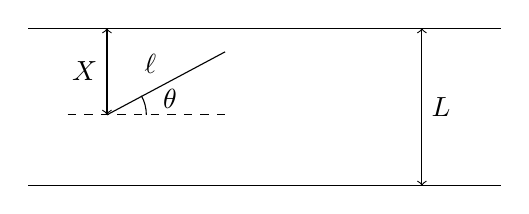
\begin{tikzpicture}
          \draw (-3, -1) -- (3, -1);
          \draw (-3, 1) -- (3, 1);
          \draw (-2, -0.1) -- (-0.5, 0.7) node [anchor = south east, pos = 0.5] {$\ell$};
          \draw [->] (-2, -0.1) -- (-2, 1) node [left, pos = 0.5] {$X$};
          \draw [->] (-2, 1) -- (-2, -0.1);
          \draw [dashed] (-2.5, -0.1) -- (-0.5, -0.1);
          \draw (-1.5, -0.1) arc (0:29:0.5);
          \node at (-1.2, 0.1) {$\theta$};
          \draw [->] (2, -1) -- (2, 1) node [right, pos = 0.5] {$L$};
          \draw [->] (2, 1) -- (2, -1);
        \end{tikzpicture}
      \end{center}
      Suppose we toss the pin $n$ times, and it hits the line $N$ times. Then
      \[
        N\approx N(np, np(1 - p))
      \]
      by the Central limit theorem. Write $p'$ for the actual proportion observed. Then
      \begin{align*}
        \hat{\pi} &= \frac{2\ell}{(N/n) L} \\
        &= \frac{\pi 2\ell/(\pi L)}{p'}\\
        &= \frac{\pi p}{p + (p' - p)}\\
        &= \pi \left(1 - \frac{p' - p}{p} + \cdots \right)
      \end{align*}
      Hence
      \[
        \hat\pi - \pi \approx \frac{p - p'}{p}.
      \]
      We know
      \[
        p' \sim N\left(p, \frac{p(1 - p)}{n}\right).
      \]
      So we can find
      \[
        \hat \pi - \pi \sim N\left(0, \frac{\pi^2 p(1 - p)}{np^2}\right) = N\left(0, \frac{\pi^2(1 - p)}{np}\right)
      \]
      We want a small variance, and that occurs when $p$ is the largest. Since $p = 2\ell/\pi L$, this is maximized with $\ell = L$. In this case,
      \[
        p = \frac{2}{\pi},
      \]
      and
      \[
        \hat \pi - \pi \approx N\left(0, \frac{(\pi - 2)\pi^2}{2n}\right).
      \]
      If we want to estimate $\pi$ to 3 decimal places, then we need
      \[
        \P(|\hat \pi - \pi| \leq 0.001) \geq 0.95.
      \]
      This is true if and only if
      \[
        0.001\sqrt{\frac{2n}{(\pi - 2)(\pi^2)}} \geq \Phi^{-1}(0.975) = 1.96
      \]
      So $n\geq 2.16 \times 10^7$. So we can obtain $\pi$ to 3 decimal places just by throwing a stick 20 million times! Isn't that exciting?
    \end{eg}
  \end{field}
  \begin{field}
    \begin{eg}[Estimating $\pi$ with Buffon's needle]
      Recall that if we randomly toss a needle of length $\ell$ to a floor marked with parallel lines a distance $L$ apart, the probability that the needle hits the line is $p = \frac{2\ell}{\pi L}$.
      \begin{center}
        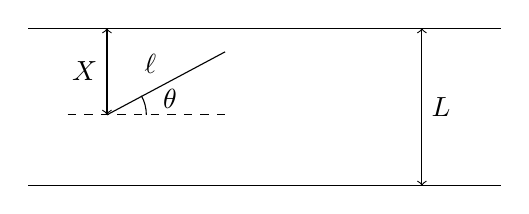
\begin{tikzpicture}
          \draw (-3, -1) -- (3, -1);
          \draw (-3, 1) -- (3, 1);
          \draw (-2, -0.1) -- (-0.5, 0.7) node [anchor = south east, pos = 0.5] {$\ell$};
          \draw [->] (-2, -0.1) -- (-2, 1) node [left, pos = 0.5] {$X$};
          \draw [->] (-2, 1) -- (-2, -0.1);
          \draw [dashed] (-2.5, -0.1) -- (-0.5, -0.1);
          \draw (-1.5, -0.1) arc (0:29:0.5);
          \node at (-1.2, 0.1) {$\theta$};
          \draw [->] (2, -1) -- (2, 1) node [right, pos = 0.5] {$L$};
          \draw [->] (2, 1) -- (2, -1);
        \end{tikzpicture}
      \end{center}
      Suppose we toss the pin $n$ times, and it hits the line $N$ times. Then
      \[
        N\approx N(np, np(1 - p))
      \]
      by the Central limit theorem. Write $p'$ for the actual proportion observed. Then
      \begin{align*}
        \hat{\pi} &= \frac{2\ell}{(N/n) L} \\
        &= \frac{\pi 2\ell/(\pi L)}{p'}\\
        &= \frac{\pi p}{p + (p' - p)}\\
        &= \pi \left(1 - \frac{p' - p}{p} + \cdots \right)
      \end{align*}
      Hence
      \[
        \hat\pi - \pi \approx \frac{p - p'}{p}.
      \]
      We know
      \[
        p' \sim N\left(p, \frac{p(1 - p)}{n}\right).
      \]
      So we can find
      \[
        \hat \pi - \pi \sim N\left(0, \frac{\pi^2 p(1 - p)}{np^2}\right) = N\left(0, \frac{\pi^2(1 - p)}{np}\right)
      \]
      We want a small variance, and that occurs when $p$ is the largest. Since $p = 2\ell/\pi L$, this is maximized with $\ell = L$. In this case,
      \[
        p = \frac{2}{\pi},
      \]
      and
      \[
        \hat \pi - \pi \approx N\left(0, \frac{(\pi - 2)\pi^2}{2n}\right).
      \]
      If we want to estimate $\pi$ to 3 decimal places, then we need
      \[
        \P(|\hat \pi - \pi| \leq 0.001) \geq 0.95.
      \]
      This is true if and only if
      \[
        0.001\sqrt{\frac{2n}{(\pi - 2)(\pi^2)}} \geq \Phi^{-1}(0.975) = 1.96
      \]
      So $n\geq 2.16 \times 10^7$. So we can obtain $\pi$ to 3 decimal places just by throwing a stick 20 million times! Isn't that exciting?
    \end{eg}
  \end{field}
  \xplain{6.5 Multivariate normal}% Subsection
  \xplain{7 Central limit theorem}% Section
  \xplain{}% Subject
  \xplain{GENERAL KNOWLEDGE}% Label
\end{note}

\section{Summary of distributions}

\subsection{Discrete distributions}

\subsection{Continuous distributions}
\end{document}
